%{Backgrounds and systematics}
\section{Backgrounds}
While the VBF $H\rightarrow WW\rightarrow \ell\nu\ell\nu$ channel gives a fairly clear signal with $E_{\text{T}}^{\text{miss}}$, two leptons, and 2 jets, there are substantial backgrounds with similar final states. These include Drell-Yan processes (in which a $Z$ boson is formed from quark anti-quark annihilation of the two colliding protons), top quark final states (predominantly $t\bar{t}$), diboson events (led by SM $WW$ events), Higgs decays from the other production modes (mainly ggF), and background from mis-identified leptons, called fakes. In this section I will detail each background and describe our methods for estimating their role in overall results. I will describe how this analysis estimates and minimizes contributions from each background process. Finally, I demonstrate purity and modelling of these backgrounds in validation and control regions. I made key contributions in this analysis in optimizing and testing control region definitions and their effects on our overall results. 

\subsection{Drell-Yan background ($Z\rightarrow \tau\tau$)}
The Drell-Yan background, alternatively called $Z\rightarrow \tau\tau$ or $Z+$jets is produced in the initial collision when two quarks produce a $Z$ boson which then decays to two leptons (in the largest background, $\tau$ leptons which then decay to electron/muons and neutrinos).  Thus there are two jets and two leptons in its final state as well as missing energy from neutrinos, all of which are indicative of signal VBF Higgs events as well. A typical Drell-Yan Feynman diagram is shown in Figure \ref{fig:DrellYan}. 
\begin{figure}
\centering
  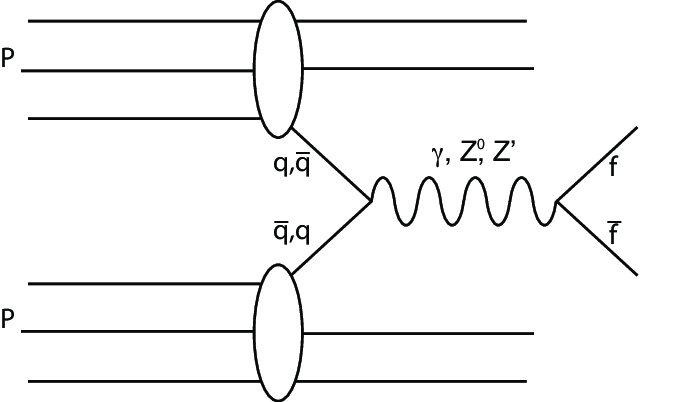
\includegraphics[width=.35\linewidth]{Pictures/FeynmanDrellYan.png}
\caption{Feynman diagram for Drell-Yan process in which two quarks produce a photon or $Z$-boson that then decays leptonically \cite{DrellYan}.}
\label{fig:DrellYan}
\end{figure}
The Drell-Yan background can be discriminated from our signal as well as the other backgrounds in two main ways- first in terms of the mass of the overall event aligning with the mass of the $Z$ boson. To select for Drell-Yan events we can select those which $m_{\tau\tau}$ is near the $Z$ mass peak. $m_{\tau\tau}$ is defined in the previous section and cutting on this in a 25 GeV window about the $Z$-mass peak drasticly improves our $Z+$jets purity from only 19$\%$ of total events to $\approx52\%$. 

We have also tested and trained a secondary discriminant for $Z+$jets in our analysis, a BDT trained to discriminate $Z+$jets and VBF signal events. This BDT significantly decreases overall $Z+$jets background in our signal region but we found that the subsequent decrease in statistics from using this cut leads to very similar overall results. The results from this comparison are shown in the Appendix. 

\subsubsection{Drell-Yan Control Region}

The $Z+$jets control region definition is quite similar to the VBF signal region except that the $Z+$jets veto cut is inverted. Thus instead of removing events near the $Z$-mass window we select for them by applying a cut on $m_{ll}<80$ GeV,  66.2 GeV $< m_{\tau\tau}< 116.2$ GeV, and the same OLV and CJV cuts as in the VBF signal region. The $Z+$jets control region has a purity of $\approx 82\%$ and yields in this region are shown in the table below.

\begin{table}[h!]
\scalebox{0.35}{
%%% created on Sat Apr 18 17:21:56 2020 from TQSampleFolder 'samples' with TQLibrary UNKNOWN compiled with GCC 8.3.0 against ROOT 6.16/00
\providecommand{\xmark}{{\sffamily \bfseries X}}
\providecommand\rotatecell[2]{\rotatebox[origin=c]{#1}{#2}}
\begin{tabular}{ r || r  r | r  r || r  r  r | r  r  r  r }
\ensuremath{\sqrt{s}=13 TeV}, \ensuremath{\mathcal{L}=139 fb^{-1}}  (Full~Run~2) & $H_{VBF}$ & $H_{ggF}$ & $WW$ & Other VV & Top & Zjets & Mis-Id & Total Bkg & Significance & Data & Data/MC\tabularnewline
\hline
\textcolor{blue}{Scale factors} &  &  &  &  & \textcolor{blue}{NF = \ensuremath{0.99\pm 0.01}} & \textcolor{blue}{NF = \ensuremath{1.03\pm 0.05}} &  & \textcolor{blue}{NFs Applied} &  &  & \tabularnewline
$Z\to\tau\tau$ CR: $\vert m_{\tau\tau}-m_Z\vert<$ 25, bVeto & \ensuremath{27.15\pm 0.16} & \ensuremath{67.22\pm 0.76} & \ensuremath{1809.83\pm 8.26} & \ensuremath{394.27\pm 4.91} & \ensuremath{5630.06\pm 17.10} & \ensuremath{9040.34\pm 45.91} & \ensuremath{507.91\pm 26.88} & \ensuremath{17449.63\pm 56.70} & \ensuremath{0.21\pm 0.00} & \ensuremath{16400} & \ensuremath{0.94\pm 0.01}\tabularnewline
\textcolor{blue}{Scale factors} &  &  &  &  & \textcolor{blue}{NF = \ensuremath{0.99\pm 0.01}} & \textcolor{blue}{NF = \ensuremath{1.03\pm 0.05}} &  & \textcolor{blue}{NFs Applied} &  &  & \tabularnewline
$Z\to\tau\tau$ CR: $M_{ll}<80$ GeV & \ensuremath{26.48\pm 0.16} & \ensuremath{64.96\pm 0.75} & \ensuremath{589.77\pm 4.57} & \ensuremath{221.55\pm 4.43} & \ensuremath{1702.27\pm 9.24} & \ensuremath{8802.21\pm 41.65} & \ensuremath{284.22\pm 21.72} & \ensuremath{11664.97\pm 48.30} & \ensuremath{0.25\pm 0.00} & \ensuremath{10805} & \ensuremath{0.92\pm 0.01}\tabularnewline
\textcolor{blue}{Scale factors} &  &  &  &  & \textcolor{blue}{NF = \ensuremath{0.99\pm 0.01}} & \textcolor{blue}{NF = \ensuremath{1.03\pm 0.05}} &  & \textcolor{blue}{NFs Applied} &  &  & \tabularnewline
$Z\to\tau\tau$ CR: CJV$<20$ GeV & \ensuremath{20.86\pm 0.14} & \ensuremath{46.58\pm 0.63} & \ensuremath{419.89\pm 3.94} & \ensuremath{161.68\pm 4.14} & \ensuremath{1149.53\pm 7.66} & \ensuremath{6569.13\pm 36.52} & \ensuremath{224.08\pm 18.68} & \ensuremath{8570.90\pm 42.12} & \ensuremath{0.23\pm 0.00} & \ensuremath{7931} & \ensuremath{0.92\pm 0.01}\tabularnewline
\textcolor{blue}{Scale factors} &  &  &  &  & \textcolor{blue}{NF = \ensuremath{0.99\pm 0.01}} & \textcolor{blue}{NF = \ensuremath{1.03\pm 0.05}} &  & \textcolor{blue}{NFs Applied} &  &  & \tabularnewline
$Z\to\tau\tau$ CR: OLV & \ensuremath{16.04\pm 0.12} & \ensuremath{11.63\pm 0.32} & \ensuremath{86.60\pm 1.87} & \ensuremath{34.00\pm 1.35} & \ensuremath{291.98\pm 3.89} & \ensuremath{1413.62\pm 17.49} & \ensuremath{30.62\pm 8.22} & \ensuremath{1868.45\pm 19.85} & \ensuremath{0.37\pm 0.00} & \ensuremath{1832} & \ensuremath{0.97\pm 0.02}\tabularnewline
\textcolor{blue}{Scale factors} &  &  &  &  & \textcolor{blue}{NF = \ensuremath{0.99\pm 0.01}} & \textcolor{blue}{NF = \ensuremath{1.03\pm 0.05}} &  & \textcolor{blue}{NFs Applied} &  &  & \tabularnewline
BDT Zjets > 0.5 & \ensuremath{3.52\pm 0.06} & \ensuremath{4.42\pm 0.20} & \ensuremath{34.38\pm 1.27} & \ensuremath{13.76\pm 1.03} & \ensuremath{106.25\pm 2.36} & \ensuremath{809.42\pm 14.54} & \ensuremath{9.33\pm 6.18} & \ensuremath{977.56\pm 16.06} & \ensuremath{0.11\pm 0.00} & \ensuremath{979} & \ensuremath{1.00\pm 0.04}\tabularnewline
\end{tabular}

}
\caption{Cutflow in the $Z+$jets control region.}
\label{tab:zttcr}
\end{table}

Data/MC shows decent agreement over various variable distributions as seen in the  below. Some of these variables are those used in the BDT described in Appendix A. 

\begin{figure}[!h]
\centering
  \subfloat[$m_{\tau\tau}$]{
      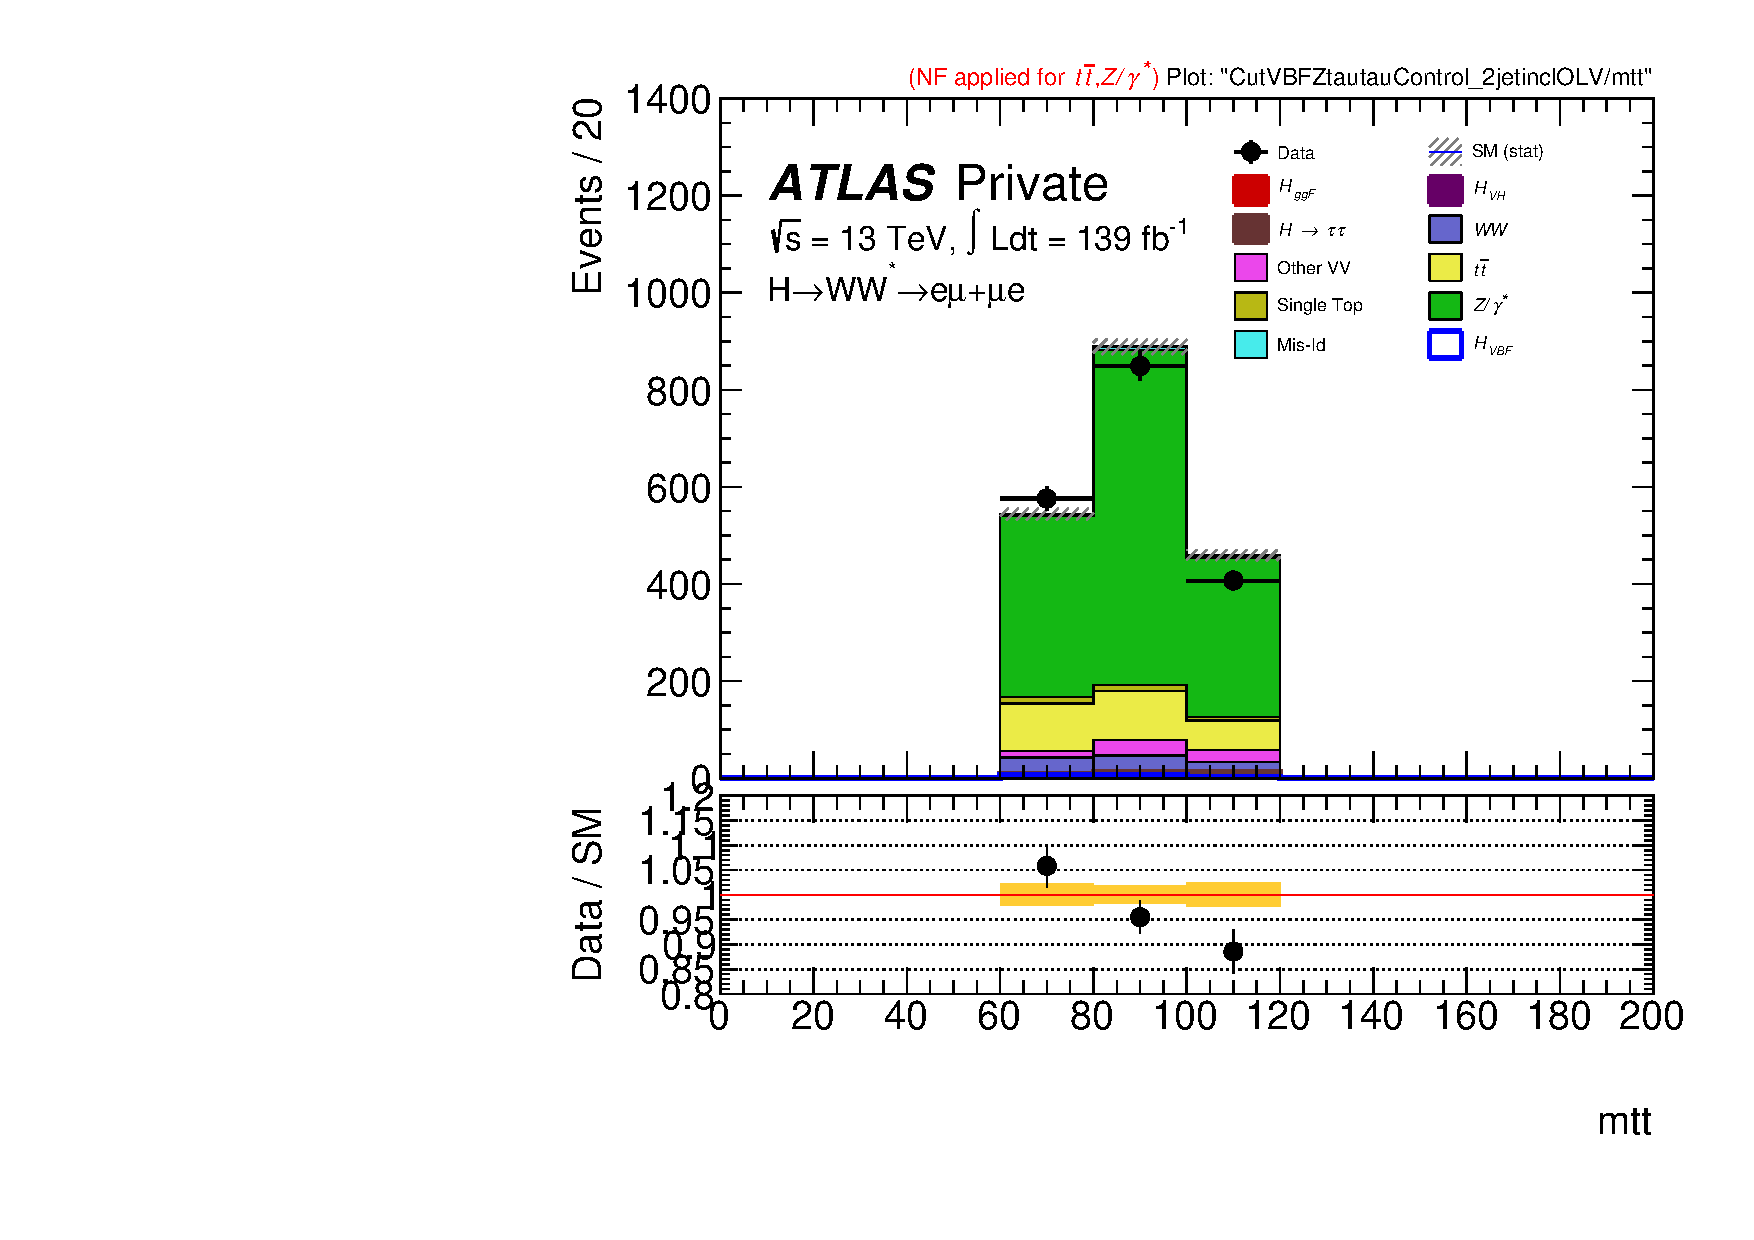
\includegraphics[width=0.3\textwidth]{Pictures/run2-emme-CutVBFZtautauControl_2jetinclOLV-mtt-lin.pdf}
  }\hfill
  \subfloat[$p^T_{tot}$]{
      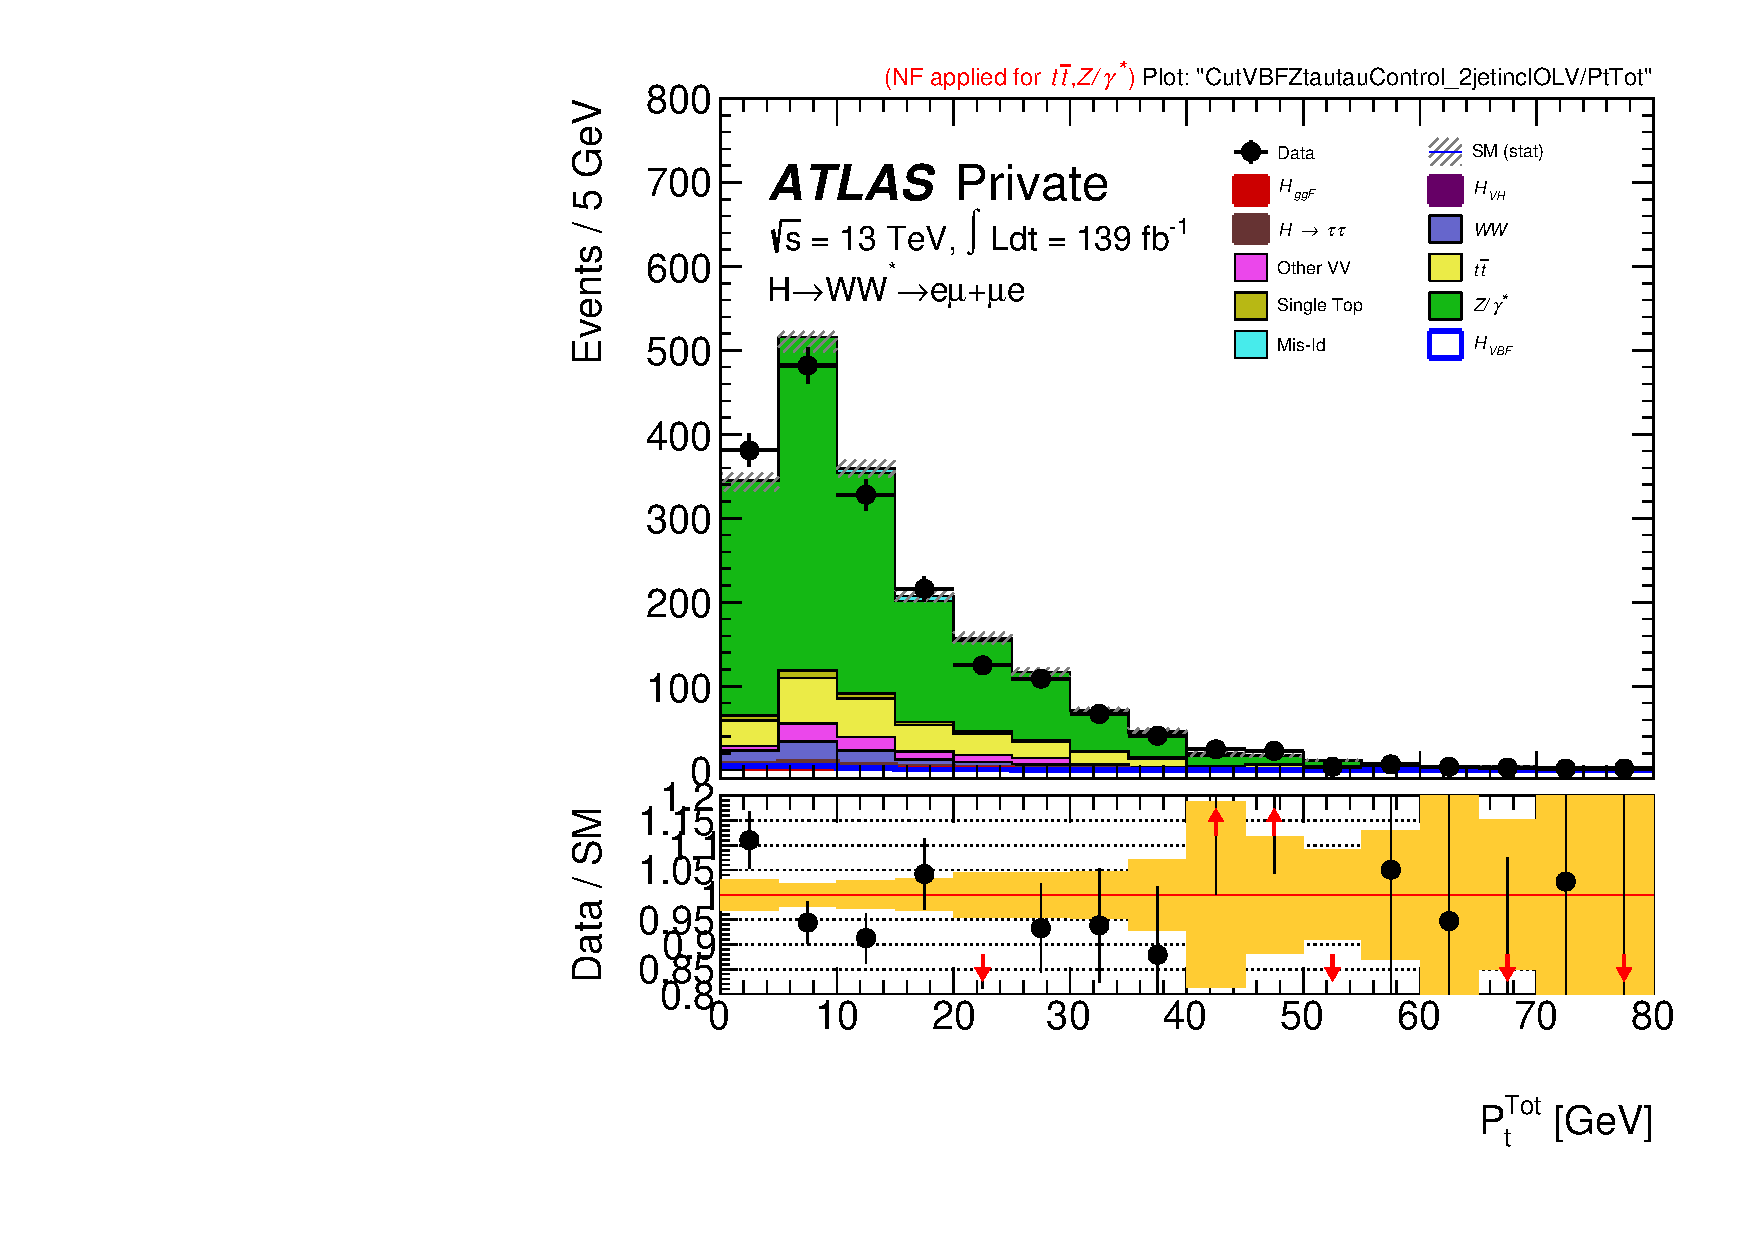
\includegraphics[width=0.3\textwidth]{Pictures/run2-emme-CutVBFZtautauControl_2jetinclOLV-PtTot-lin.pdf}
  }\hfill
  \subfloat[$m_T$]{
      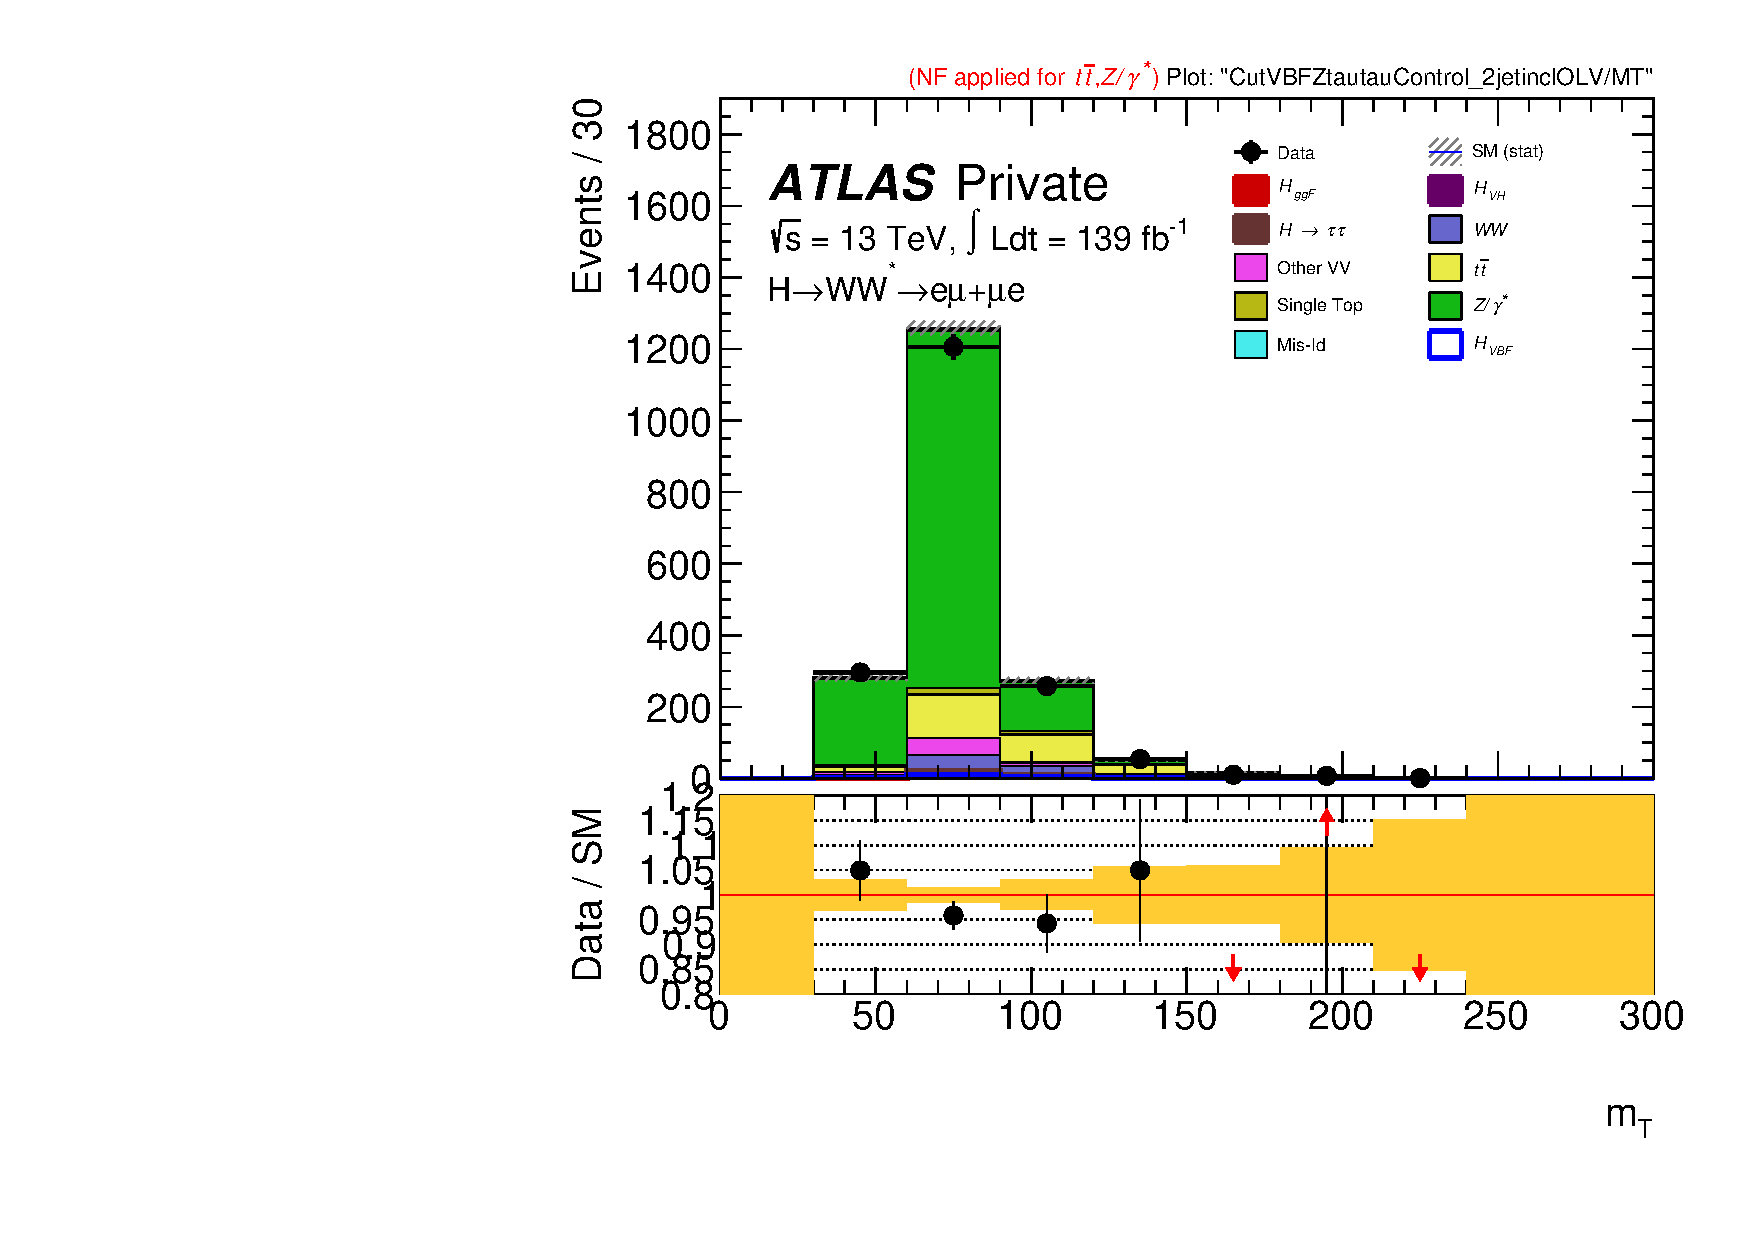
\includegraphics[width=0.3\textwidth]{Pictures/run2-emme-CutVBFZtautauControl_2jetinclOLV-MT-lin.pdf}
  }\hfill
  \subfloat[$E_{\text{T}}^{\text{miss}}$]{
      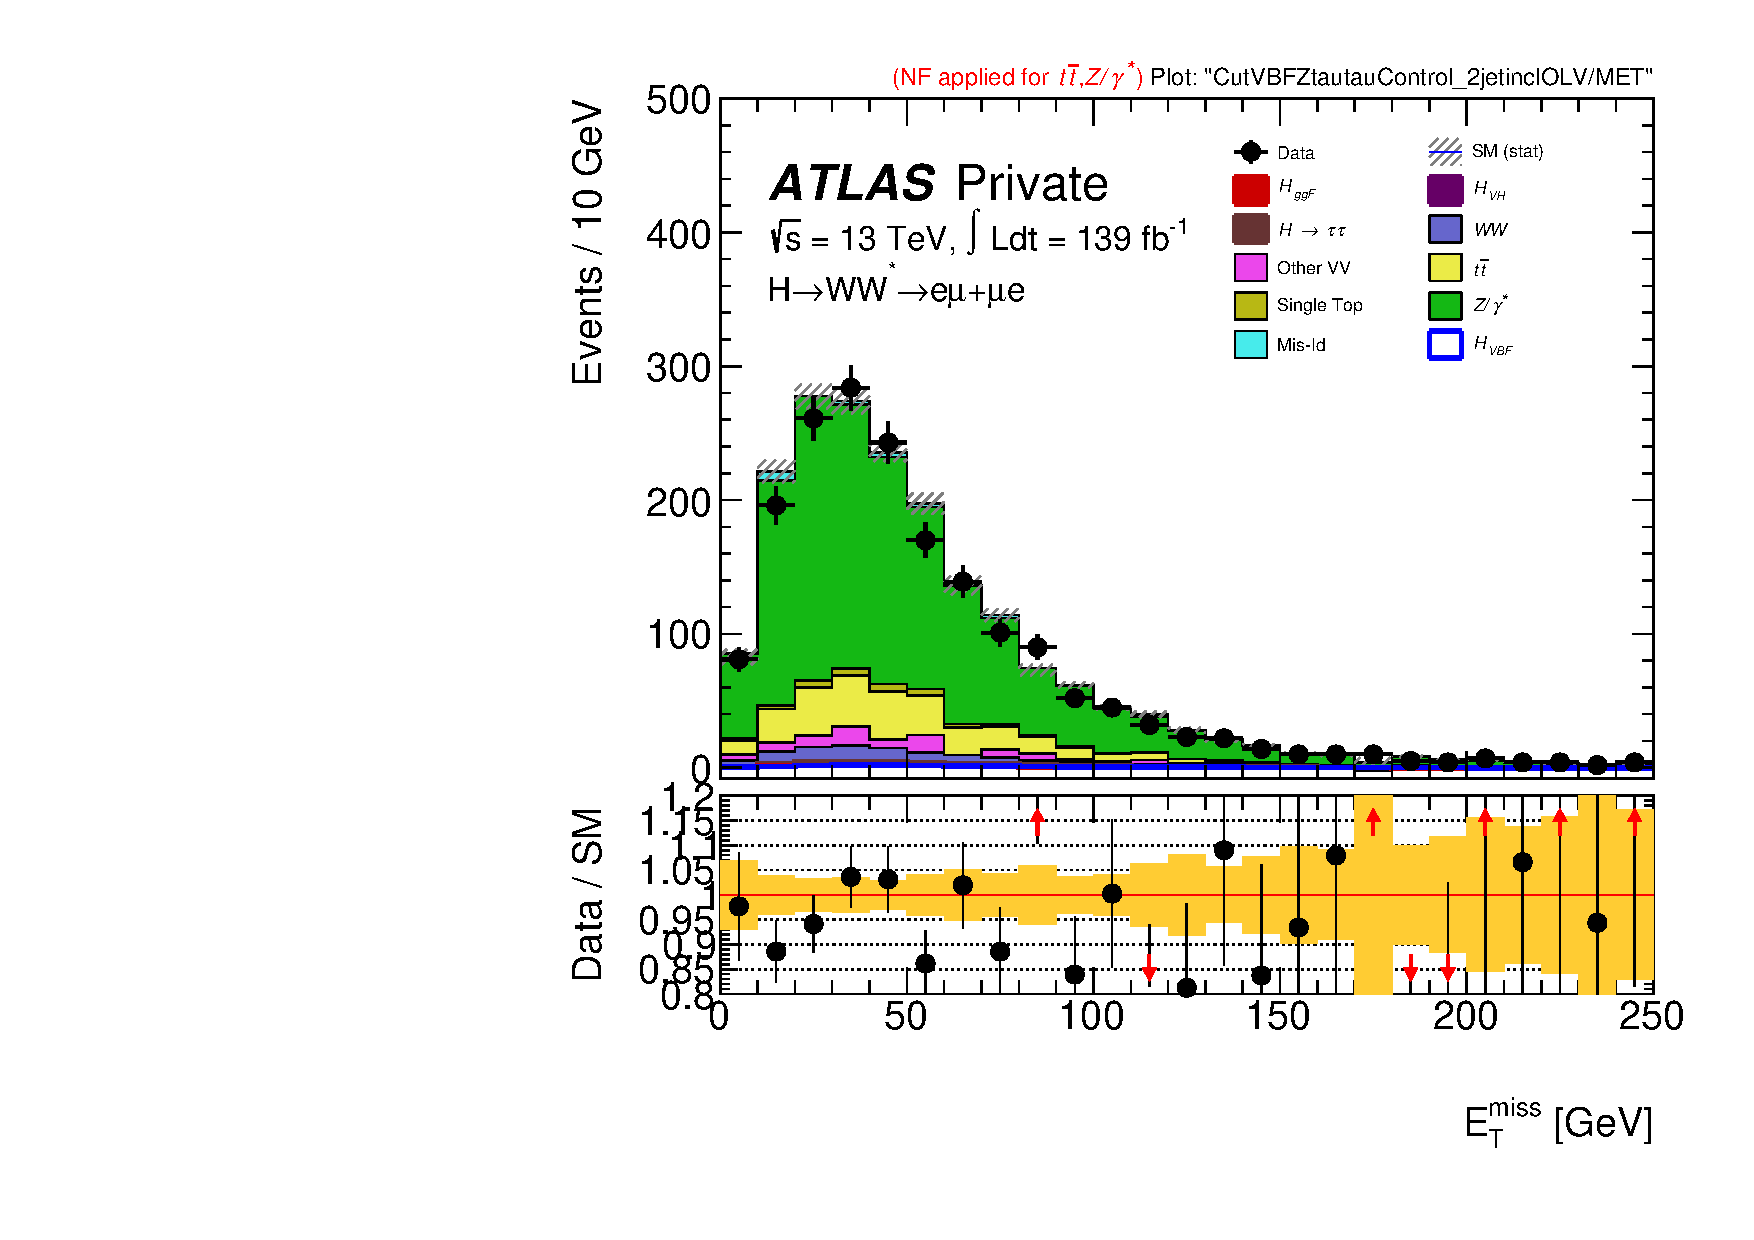
\includegraphics[width=0.3\textwidth]{Pictures/run2-emme-CutVBFZtautauControl_2jetinclOLV-MET-lin.pdf}
  }\hfill
  \subfloat[$\ensuremath{E_{\text{T,rel}}^{\text{miss}}}$]{
      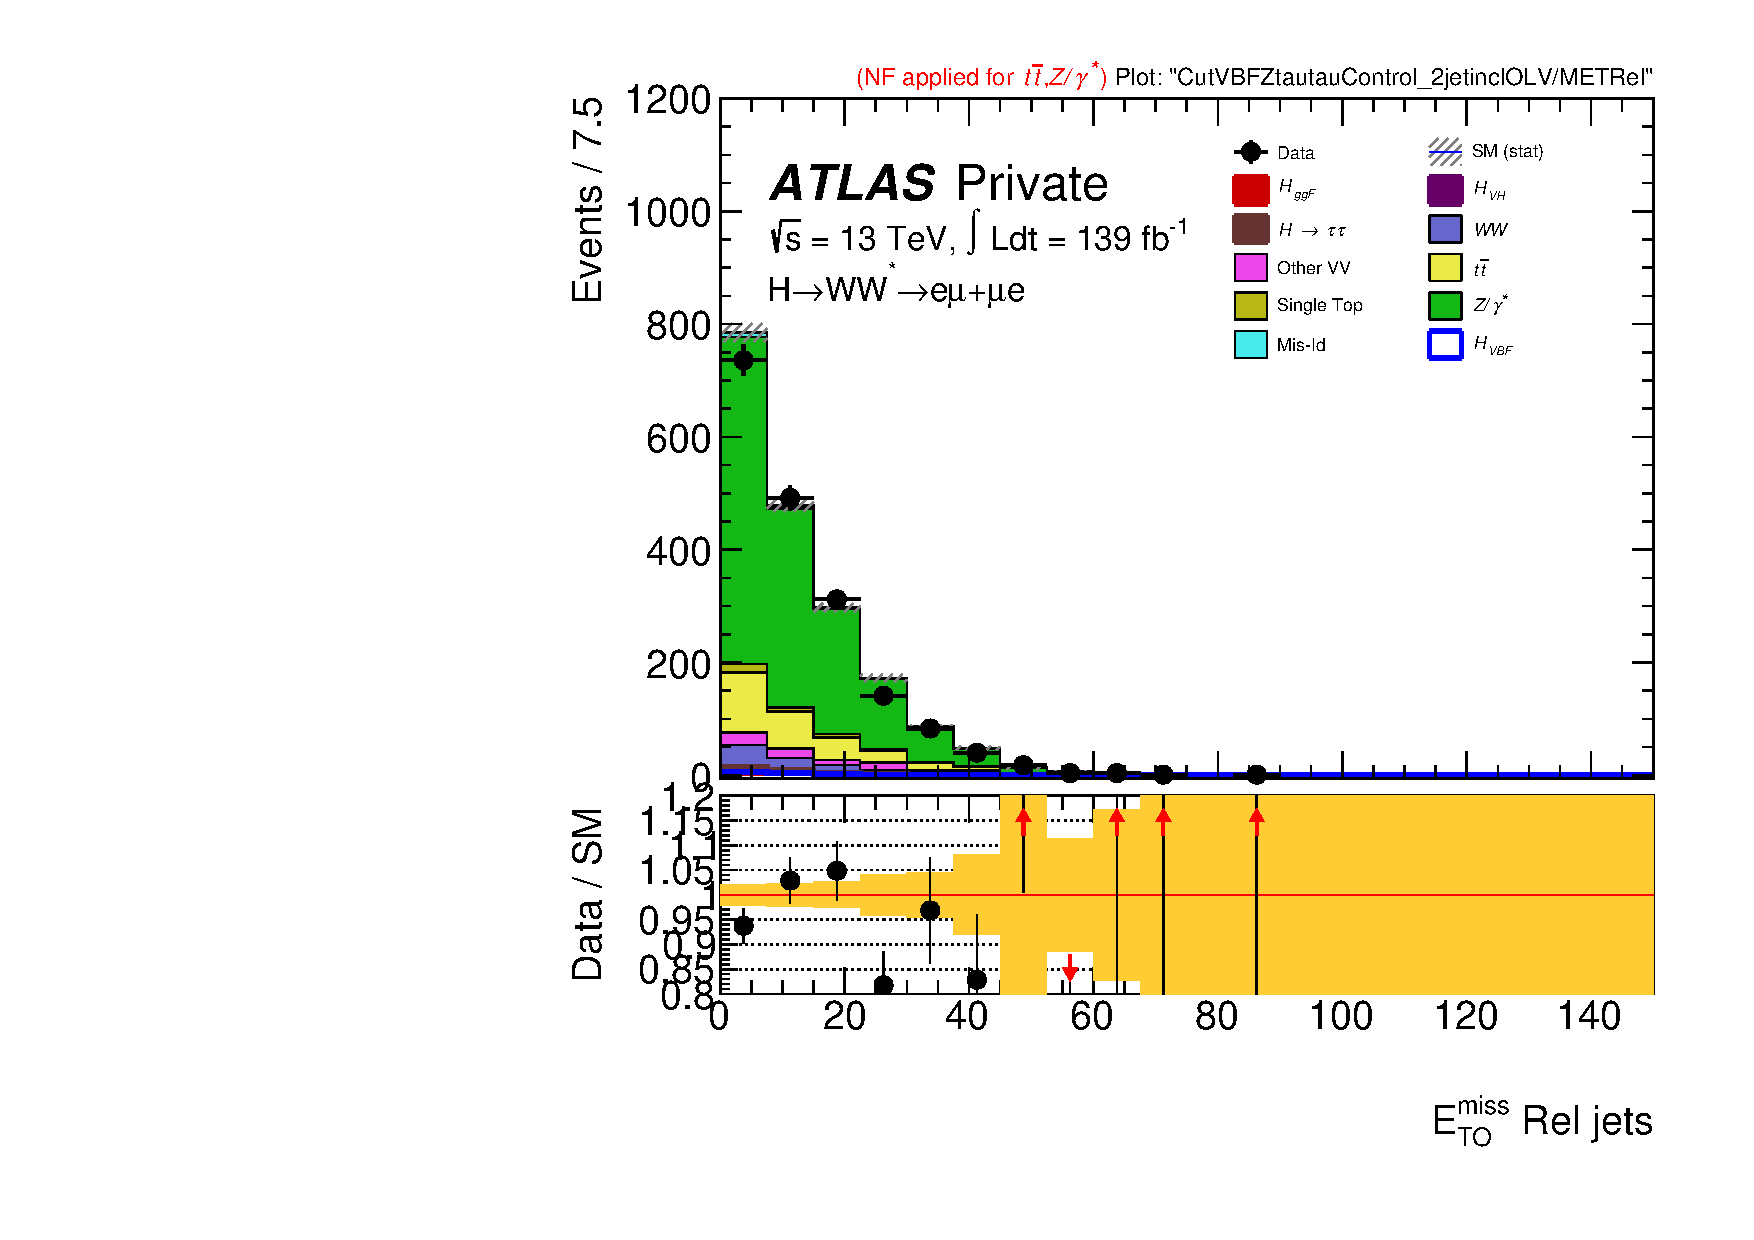
\includegraphics[width=0.3\textwidth]{Pictures/run2-emme-CutVBFZtautauControl_2jetinclOLV-METRel-lin.pdf}
  }\hfill
  \subfloat[$\ensuremath{E_{\text{T}}^{\text{miss, significance}}}$]{
      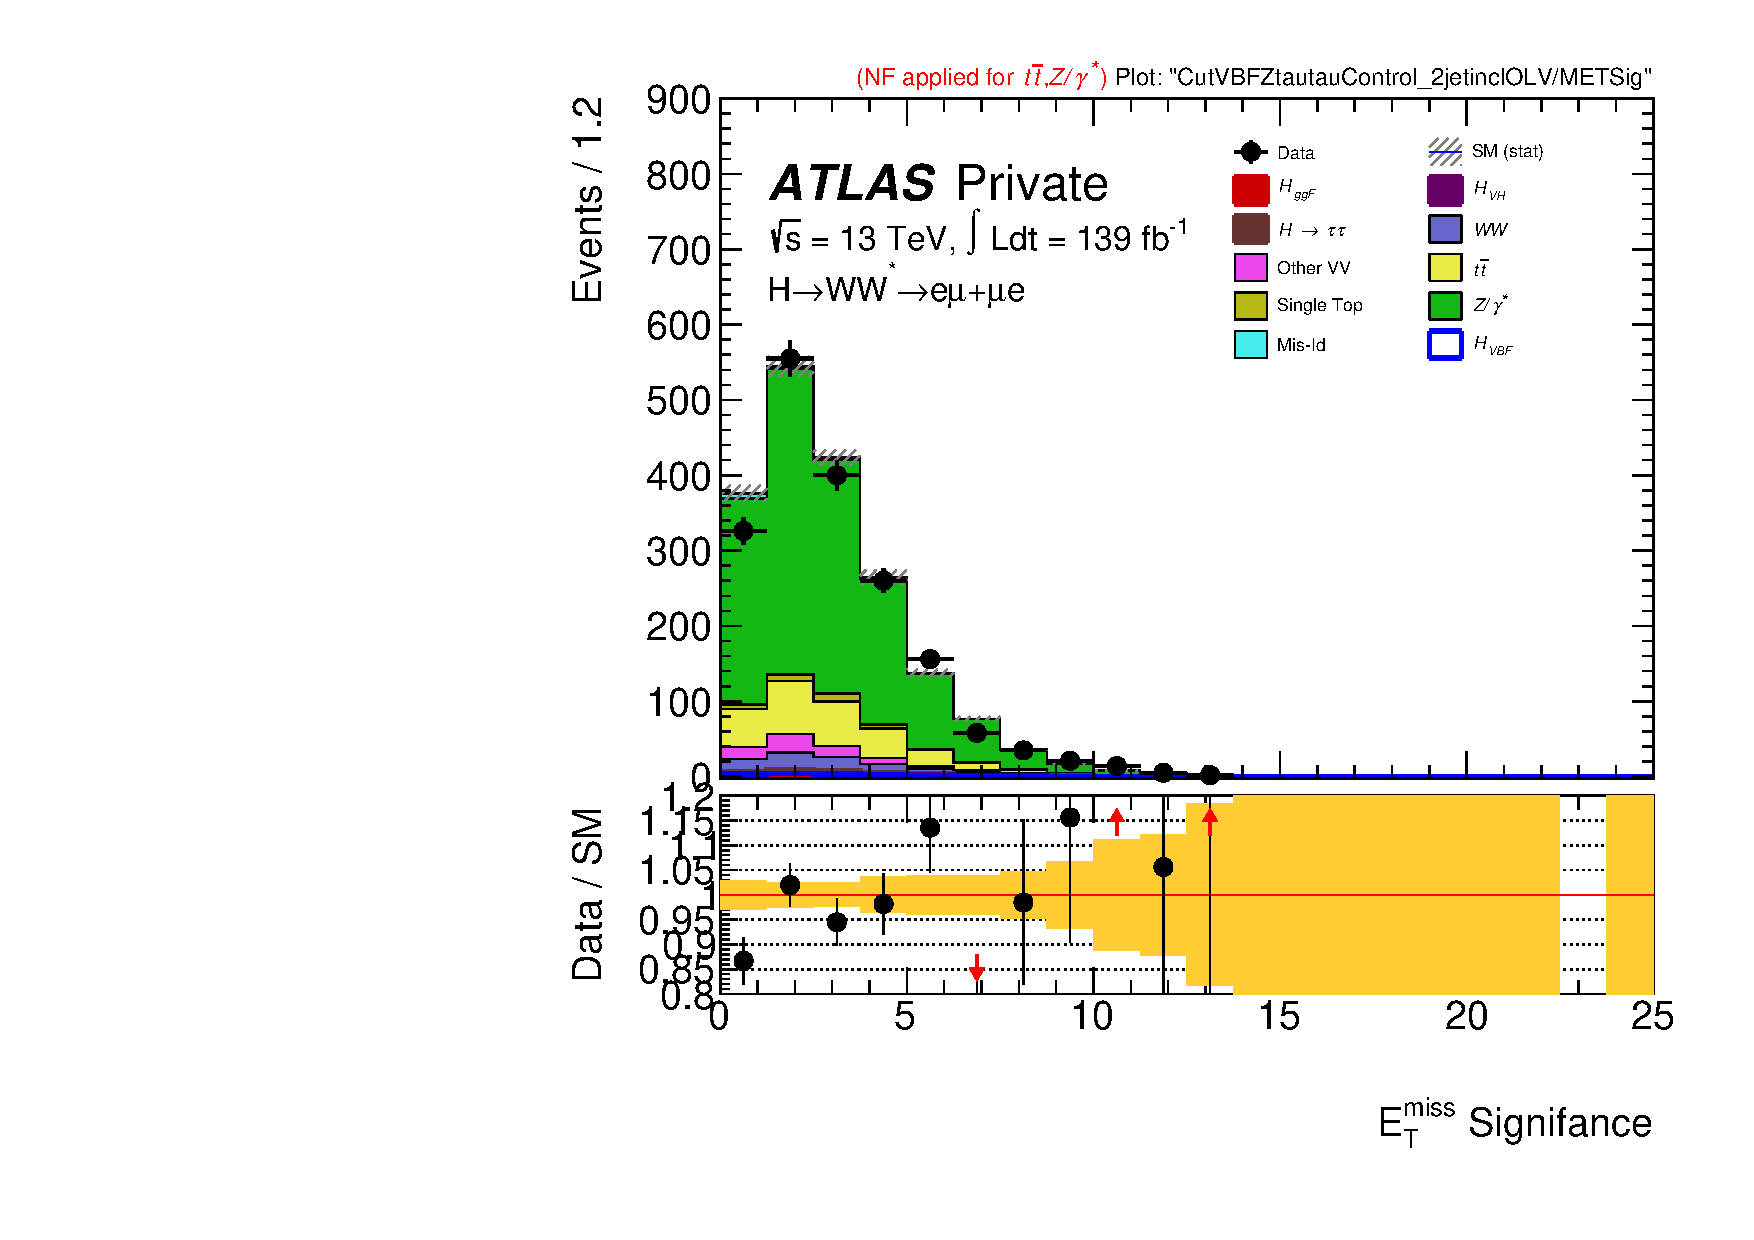
\includegraphics[width=0.3\textwidth]{Pictures/run2-emme-CutVBFZtautauControl_2jetinclOLV-METSig-lin.pdf}
  }\hfill
  \subfloat[$\ensuremath{E_{\text{T}}^{\text{miss, track}}}$]{
      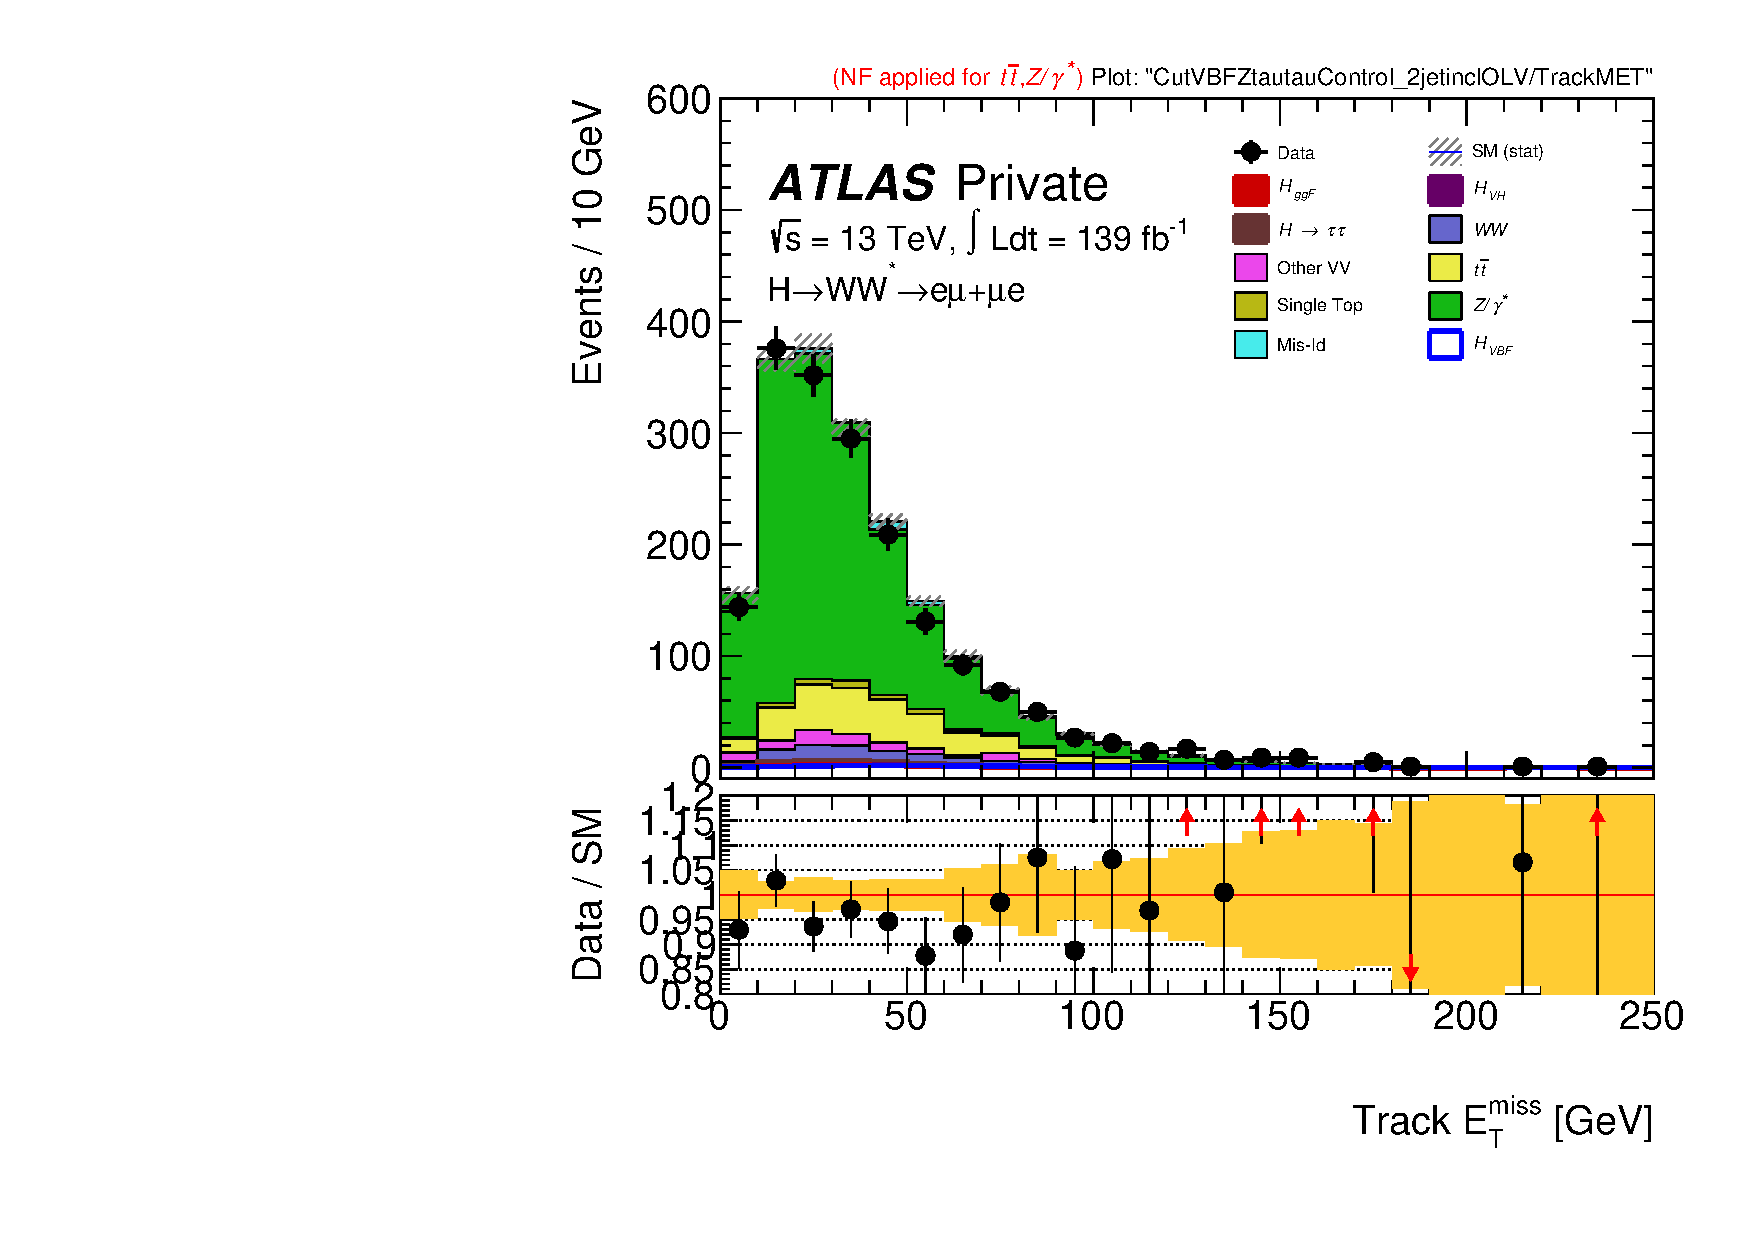
\includegraphics[width=0.3\textwidth]{Pictures/run2-emme-CutVBFZtautauControl_2jetinclOLV-TrackMET-lin.pdf}
  }\hfill
  \subfloat[$\ensuremath{E_{\text{T,rel}}^{\text{miss, track}}}$]{
      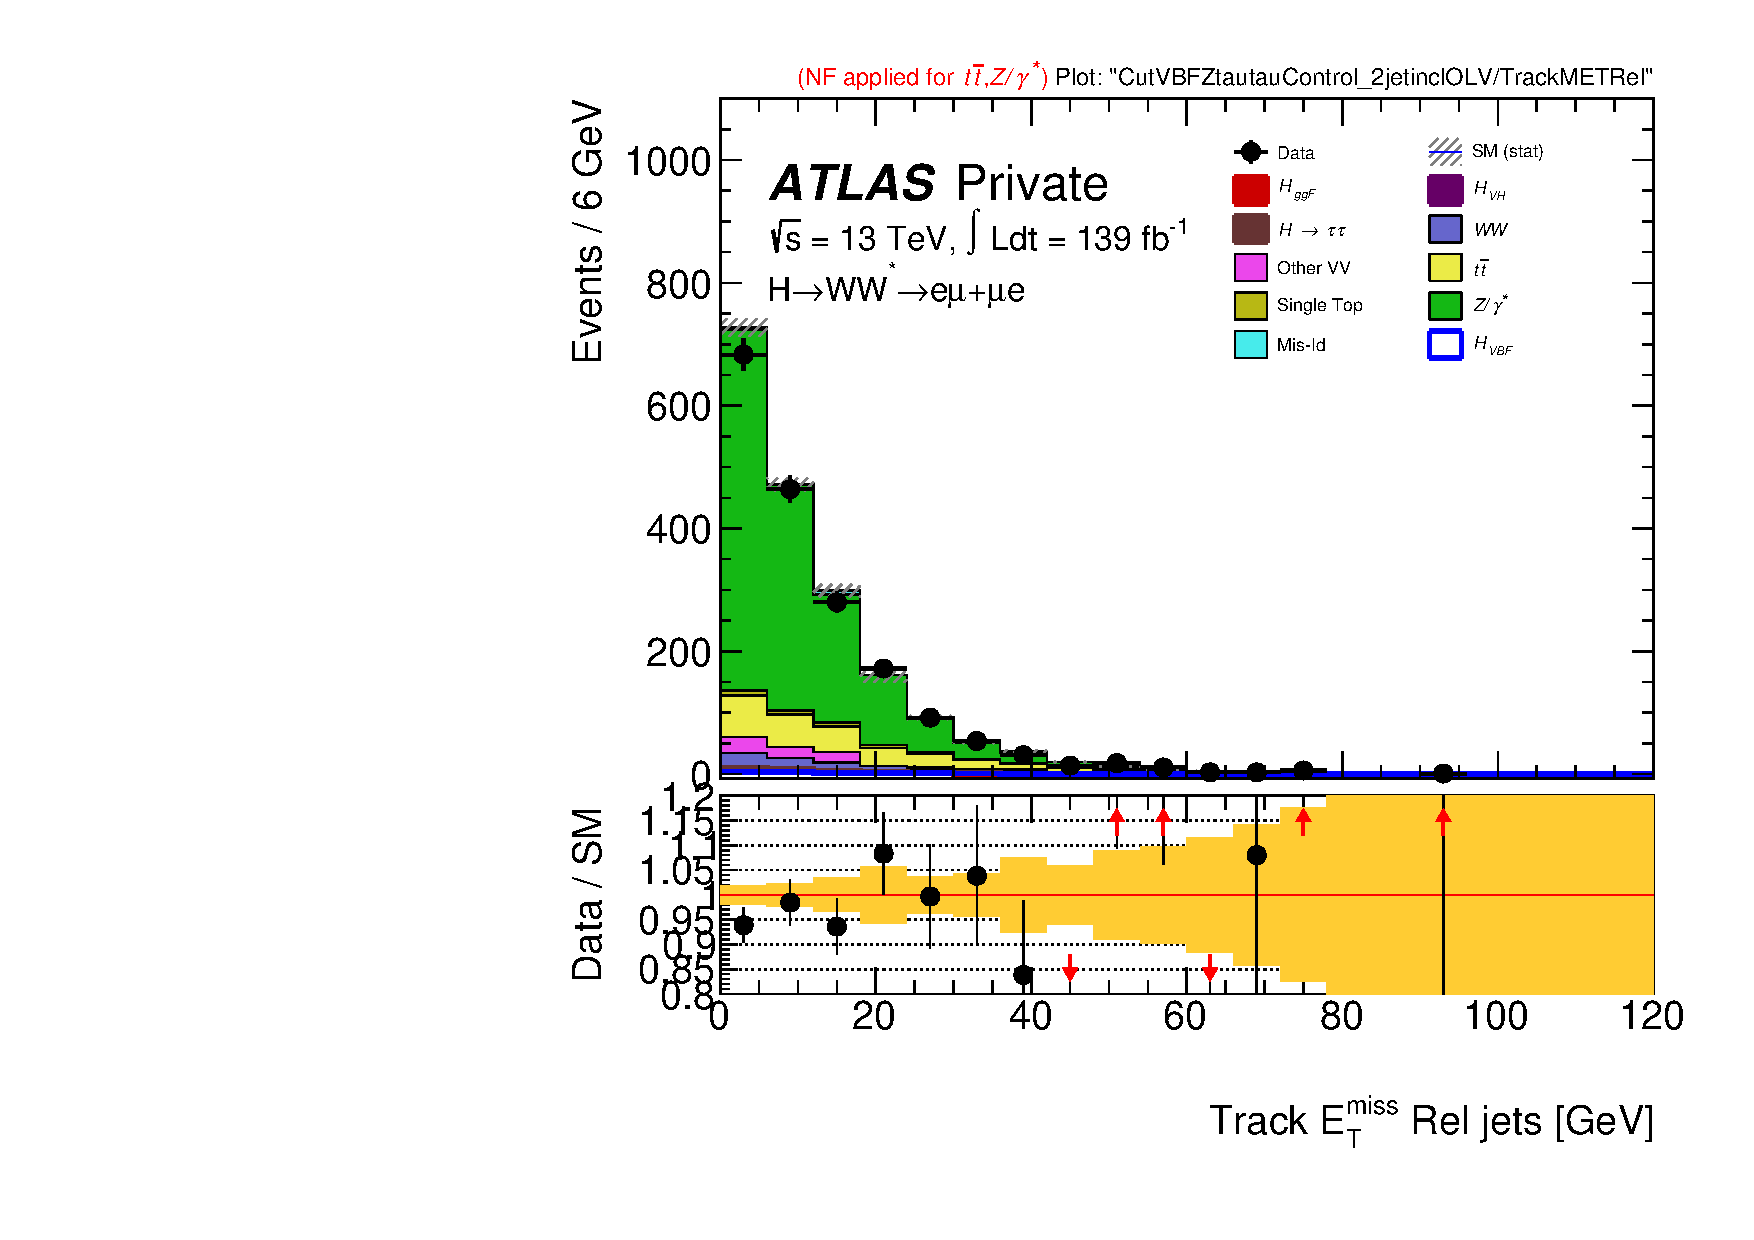
\includegraphics[width=0.3\textwidth]{Pictures/run2-emme-CutVBFZtautauControl_2jetinclOLV-TrackMETRel-lin.pdf}
  }%\hfill
 % \subfloat[$\ensuremath{\Delta\phi_{\ell\ell,E_{\text{T}}^{\text{miss, track}}}}$]{
 %     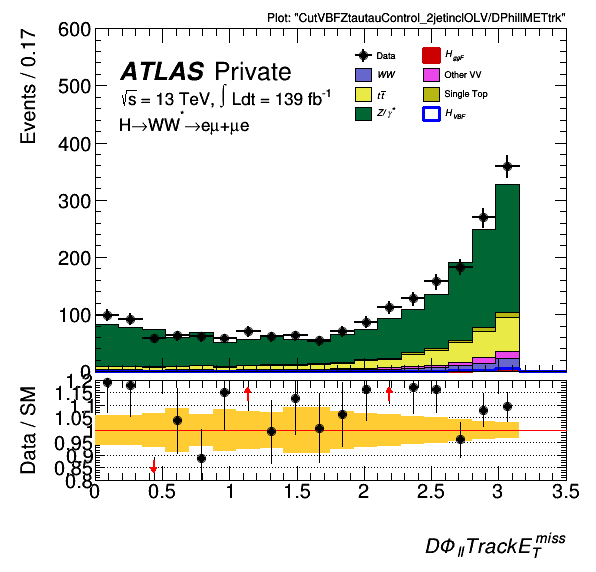
\includegraphics[width=0.3\textwidth]{Pictures/run2-emme-CutVBFZtautauControl_2jetinclOLV-DPhillMETtrk-lin.pdf}
 % }%\hfill 
{\caption{Distributions of $m_{\tau\tau}$, $p^T_{tot}$, $m_T$, $\ensuremath{E_{\text{T}}^{\text{miss}}}$, $\ensuremath{E_{\text{T, rel}}^{\text{miss}}}$, $\ensuremath{E_{\text{T}}^{\text{miss, significance}}}$, $\ensuremath{E_{\text{T}}^{\text{miss, track}}}$, and $\ensuremath{E_{\text{T,rel}}^{\text{miss, track}}}$ in the $Z+$jets control region.
\label{fig:DYCR3}}}
\end{figure}

Normalization factors (NF) are derived in the $Z+$jets control region to correct for Data/MC mis-modelling. These factors are applied to the $Z+$jets sample in the signal region. The NF factors are $1.01 \pm 0.04$. 

\subsection{Top background}
The top background consists of two main components, $Wt$ and $t\bar{t}$ events where the $W$ decays leptonically and the top quarks decay to jets (notably $b$-jets). The top background is dominated by $t\bar{t}$ and is the largest background in our signal region, composing about $60\%$ of the total background. Though top backgrounds are numerous, discrimination between top and signal Higgs events is possible through training a BDT on variables that have very different discributions between these two types of events like $m_{\ell\ell}$ and $\Delta Y_{jj}$. As demonstrated in Chapter 4, this BDT discriminates between signal and top background quite well. The top background is therefore able to be defined in the signal region and separated using dedicated discriminants. The final statistical fit is discused in the following chapter but in this section I will decribe the BDT used to isolate top background events- that splitting top$+WW$ and all other backgrounds. This is added to the overall fit as the main discriminant for top backgrounds and is considered in combination with $WW$ due to their similar signatures and their estimation as a combined parameter in the final fit.  

We also define a top validation region to test top Monte Carlo modelling as well as to calculate a normalization factor that is used to correct top mis-modelling in the signal region. The top validation region is described similarly to the signal region with one major difference, a $b$- tag applied in the signal region requiring all events with a $b$-jet to be removed is (almost) reversed. Instead we require exactly one $b$-tagged jet. We require exactly one in order to define the validation region as similarly to the signal region as possible while increasing top purity. The result is a highly pure top validation region where the flavor composition of the tagged jets is close to the signal region. Purity of the top control region is $\approx 97\%$ and yields in this region are shown in the table below.

\begin{table}[h!]
\scalebox{0.35}{
%%% created on Sat Apr 18 17:21:56 2020 from TQSampleFolder 'samples' with TQLibrary UNKNOWN compiled with GCC 8.3.0 against ROOT 6.16/00
\providecommand{\xmark}{{\sffamily \bfseries X}}
\providecommand\rotatecell[2]{\rotatebox[origin=c]{#1}{#2}}
\begin{tabular}{ r || r  r | r  r || r  r  r | r  r  r  r }
\ensuremath{\sqrt{s}=13 TeV}, \ensuremath{\mathcal{L}=139 fb^{-1}}  (Full~Run~2) & $H_{VBF}$ & $H_{ggF}$ & $WW$ & Other VV & Top & Zjets & Mis-Id & Total Bkg & Significance & Data & Data/MC\tabularnewline
\hline
\textcolor{blue}{Scale factors} &  &  &  &  & \textcolor{blue}{NF = \ensuremath{0.99\pm 0.01}} & \textcolor{blue}{NF = \ensuremath{1.03\pm 0.05}} &  & \textcolor{blue}{NFs Applied} &  &  & \tabularnewline
$n_{b-jets} = 1$ & \ensuremath{39.79\pm 0.19} & \ensuremath{129.20\pm 1.08} & \ensuremath{2993.57\pm 9.53} & \ensuremath{690.94\pm 4.40} & \ensuremath{349498.67\pm 128.68} & \ensuremath{3739.16\pm 34.69} & \ensuremath{4824.17\pm 101.77} & \ensuremath{361875.73\pm 168.02} & \ensuremath{0.07\pm 0.00} & \ensuremath{359758} & \ensuremath{0.99\pm 0.00}\tabularnewline
\textcolor{blue}{Scale factors} &  &  &  &  & \textcolor{blue}{NF = \ensuremath{0.99\pm 0.01}} & \textcolor{blue}{NF = \ensuremath{1.03\pm 0.05}} &  & \textcolor{blue}{NFs Applied} &  &  & \tabularnewline
$Z\to\tau\tau$ veto & \ensuremath{18.05\pm 0.13} & \ensuremath{18.70\pm 0.42} & \ensuremath{175.96\pm 2.68} & \ensuremath{43.24\pm 1.19} & \ensuremath{29996.21\pm 38.10} & \ensuremath{183.57\pm 8.79} & \ensuremath{287.05\pm 30.06} & \ensuremath{30704.73\pm 49.41} & \ensuremath{0.10\pm 0.00} & \ensuremath{30709} & \ensuremath{1.00\pm 0.01}\tabularnewline
\textcolor{blue}{Scale factors} &  &  &  &  & \textcolor{blue}{NF = \ensuremath{0.99\pm 0.01}} & \textcolor{blue}{NF = \ensuremath{1.03\pm 0.05}} &  & \textcolor{blue}{NFs Applied} &  &  & \tabularnewline
CJV $<20$ GeV & \ensuremath{29.69\pm 0.17} & \ensuremath{84.86\pm 0.88} & \ensuremath{1905.77\pm 7.80} & \ensuremath{454.48\pm 3.81} & \ensuremath{238439.98\pm 107.23} & \ensuremath{2524.42\pm 30.90} & \ensuremath{3083.10\pm 83.79} & \ensuremath{246492.61\pm 139.83} & \ensuremath{0.06\pm 0.00} & \ensuremath{244811} & \ensuremath{0.99\pm 0.00}\tabularnewline
\textcolor{blue}{Scale factors} &  &  &  &  & \textcolor{blue}{NF = \ensuremath{0.99\pm 0.01}} & \textcolor{blue}{NF = \ensuremath{1.03\pm 0.05}} &  & \textcolor{blue}{NFs Applied} &  &  & \tabularnewline
OLV & \ensuremath{20.85\pm 0.14} & \ensuremath{20.90\pm 0.44} & \ensuremath{294.56\pm 3.34} & \ensuremath{76.17\pm 1.52} & \ensuremath{46224.53\pm 47.42} & \ensuremath{507.30\pm 13.10} & \ensuremath{427.86\pm 36.88} & \ensuremath{47551.32\pm 61.60} & \ensuremath{0.10\pm 0.00} & \ensuremath{47182} & \ensuremath{0.99\pm 0.00}\tabularnewline
\textcolor{blue}{Scale factors} &  &  &  &  & \textcolor{blue}{NF = \ensuremath{0.99\pm 0.01}} & \textcolor{blue}{NF = \ensuremath{1.03\pm 0.05}} &  & \textcolor{blue}{NFs Applied} &  &  & \tabularnewline
$Z\to\tau\tau$ veto & \ensuremath{18.05\pm 0.13} & \ensuremath{18.70\pm 0.42} & \ensuremath{175.96\pm 2.68} & \ensuremath{43.24\pm 1.19} & \ensuremath{29996.21\pm 38.10} & \ensuremath{183.57\pm 8.79} & \ensuremath{287.05\pm 30.06} & \ensuremath{30704.73\pm 49.41} & \ensuremath{0.10\pm 0.00} & \ensuremath{30709} & \ensuremath{1.00\pm 0.01}\tabularnewline
\hline
\end{tabular}

}
\caption{Cutflow in the top control region.}
\label{tab:topcr}
\end{table}

Data/MC in the top validation region shows good agreement over various variable distributions as seen in the  below. Many of these distributions of used as inputs to the top$+WW$ BDT. 

\begin{figure}[!h]
\centering
  \subfloat[$m_{\ell\ell}$]{
      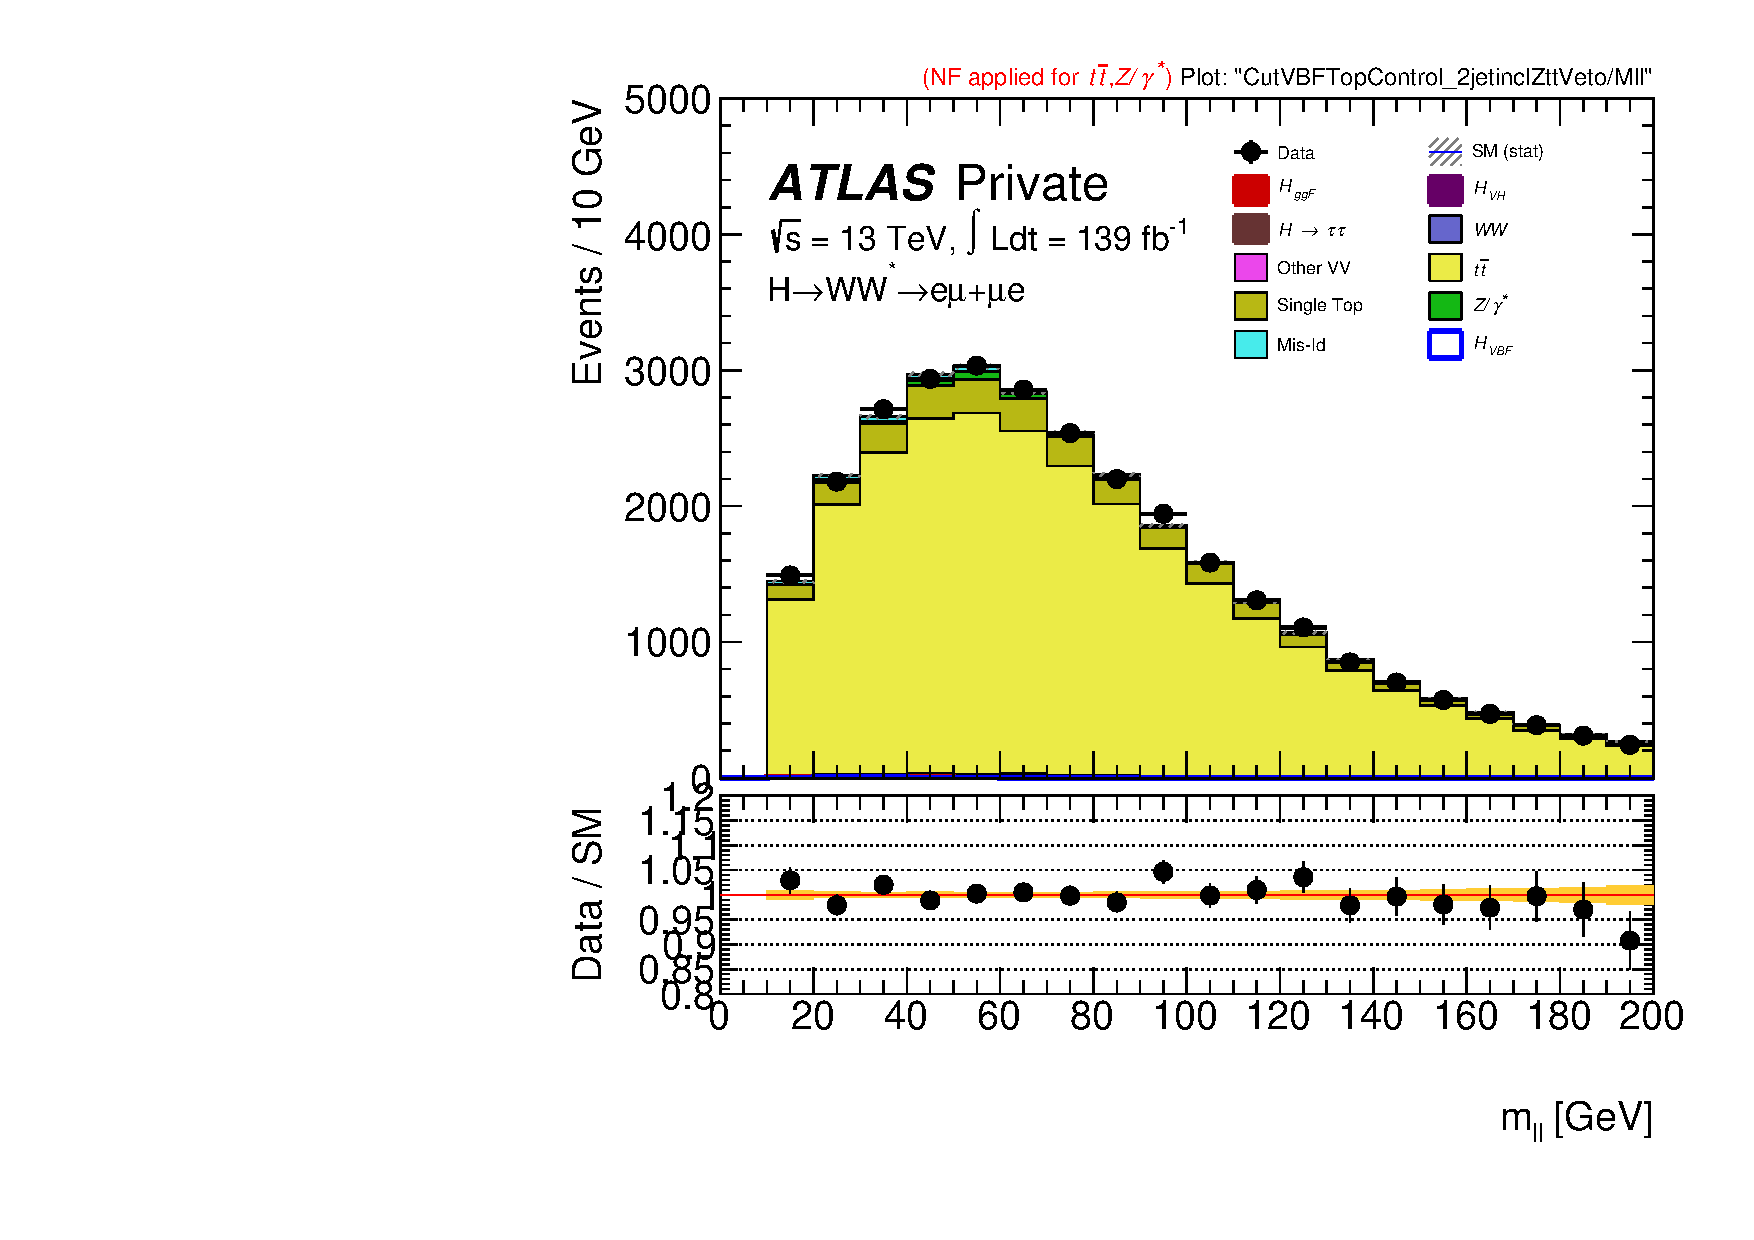
\includegraphics[width=0.3\textwidth]{Pictures/run2-emme-CutVBFTopControl_2jetinclZttVeto-Mll-lin.pdf}
  }\hfill
  \subfloat[$\Delta Y_{\ell\ell}$]{
      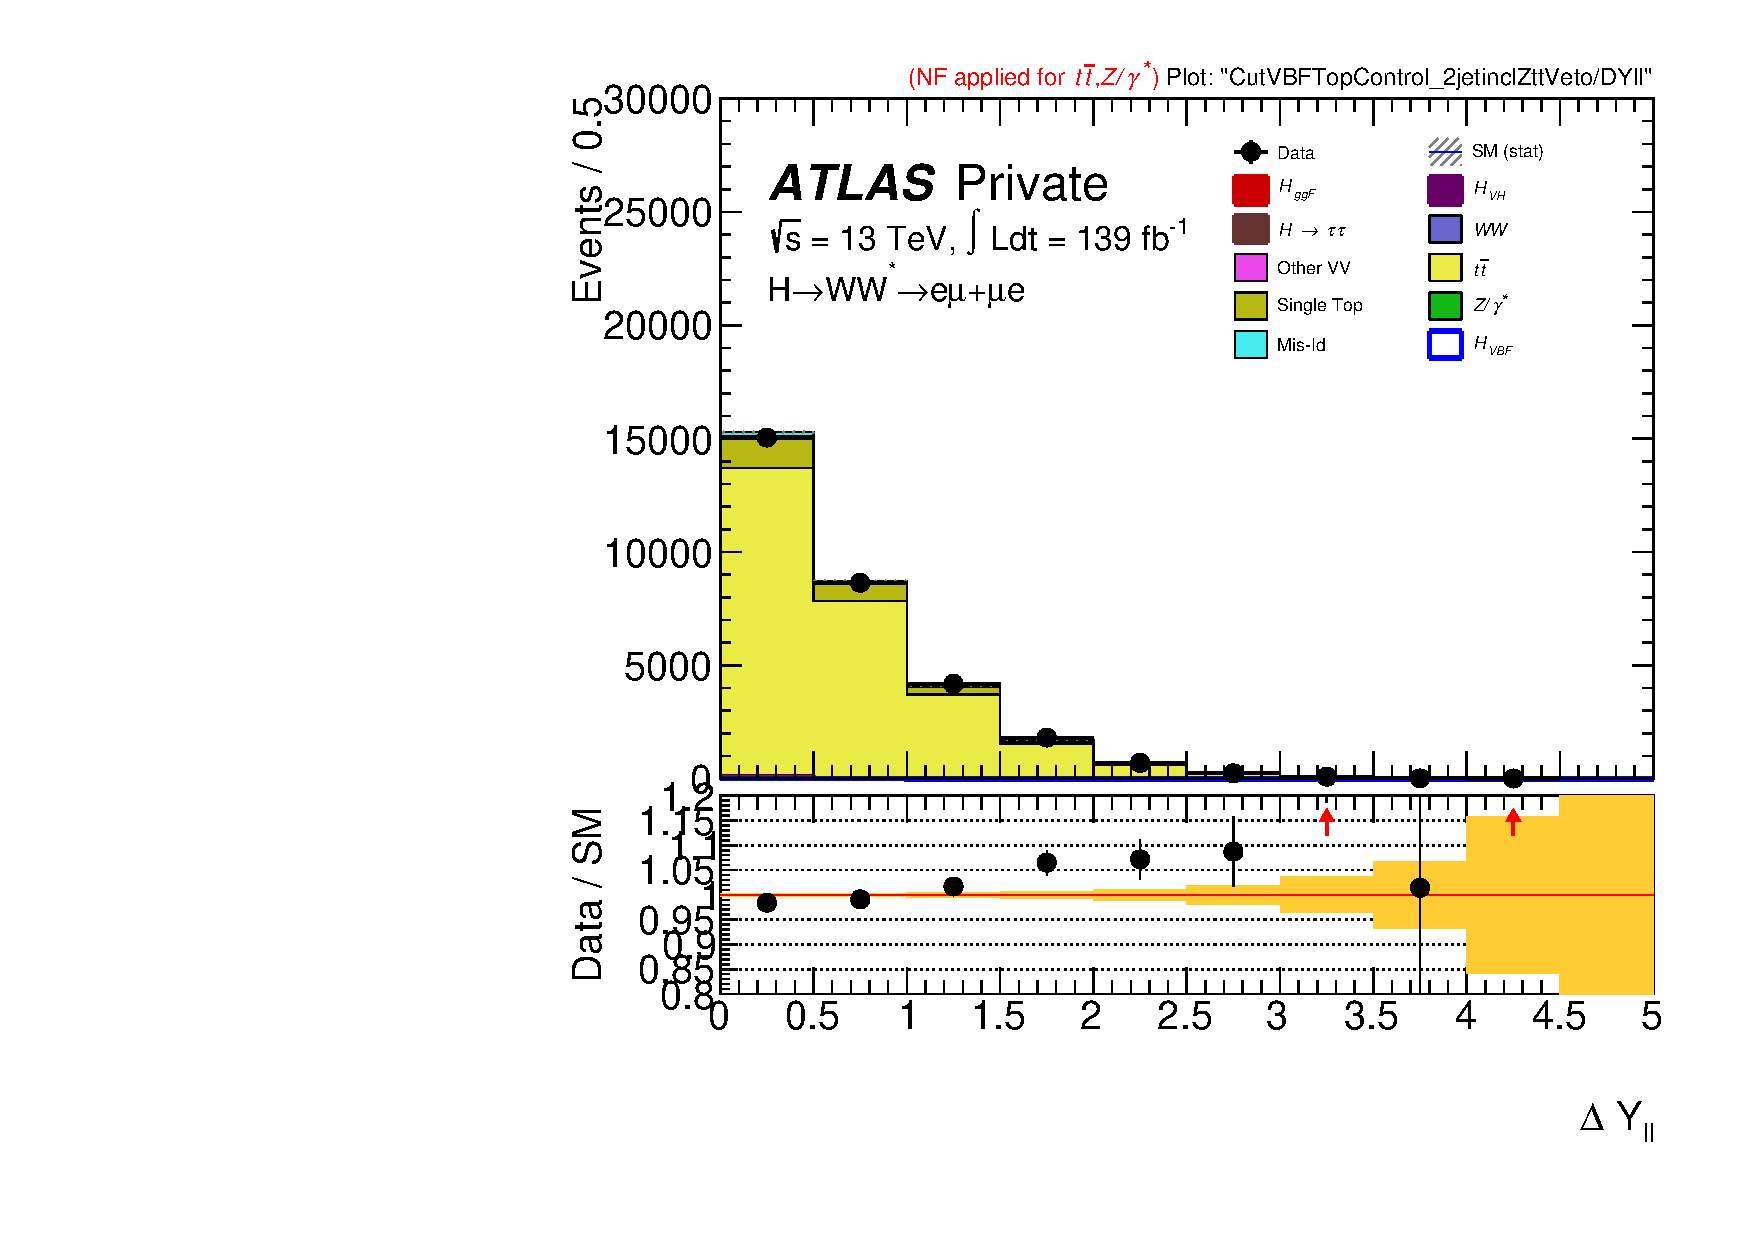
\includegraphics[width=0.3\textwidth]{Pictures/run2-emme-CutVBFTopControl_2jetinclZttVeto-DYll-lin.pdf}
  }\hfill 
  \subfloat[$\Delta Y_{jj}$]{
      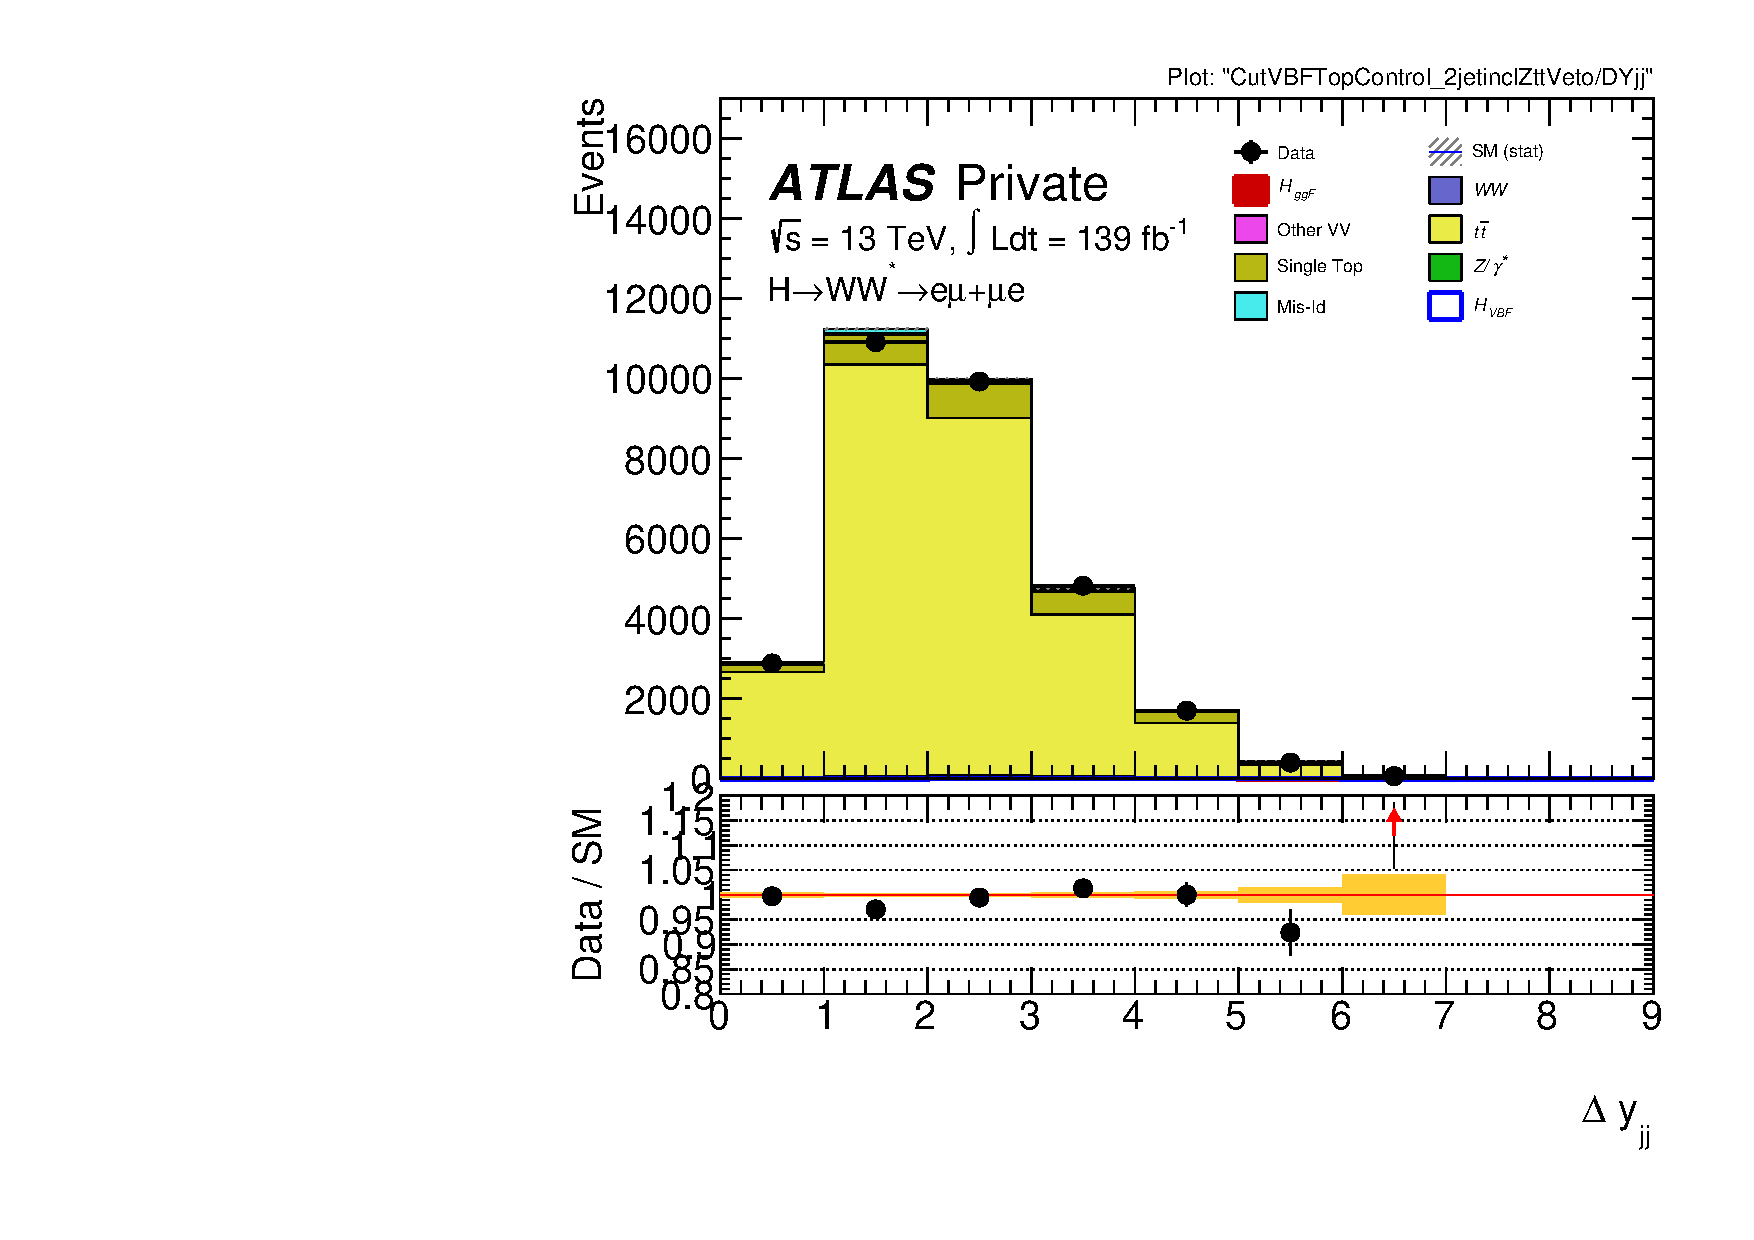
\includegraphics[width=0.3\textwidth]{Pictures/run2-emme-CutVBFTopControl_2jetinclZttVeto-DYjj-lin.pdf}
  }\hfill
  \subfloat[$\sum$ centralities]{
      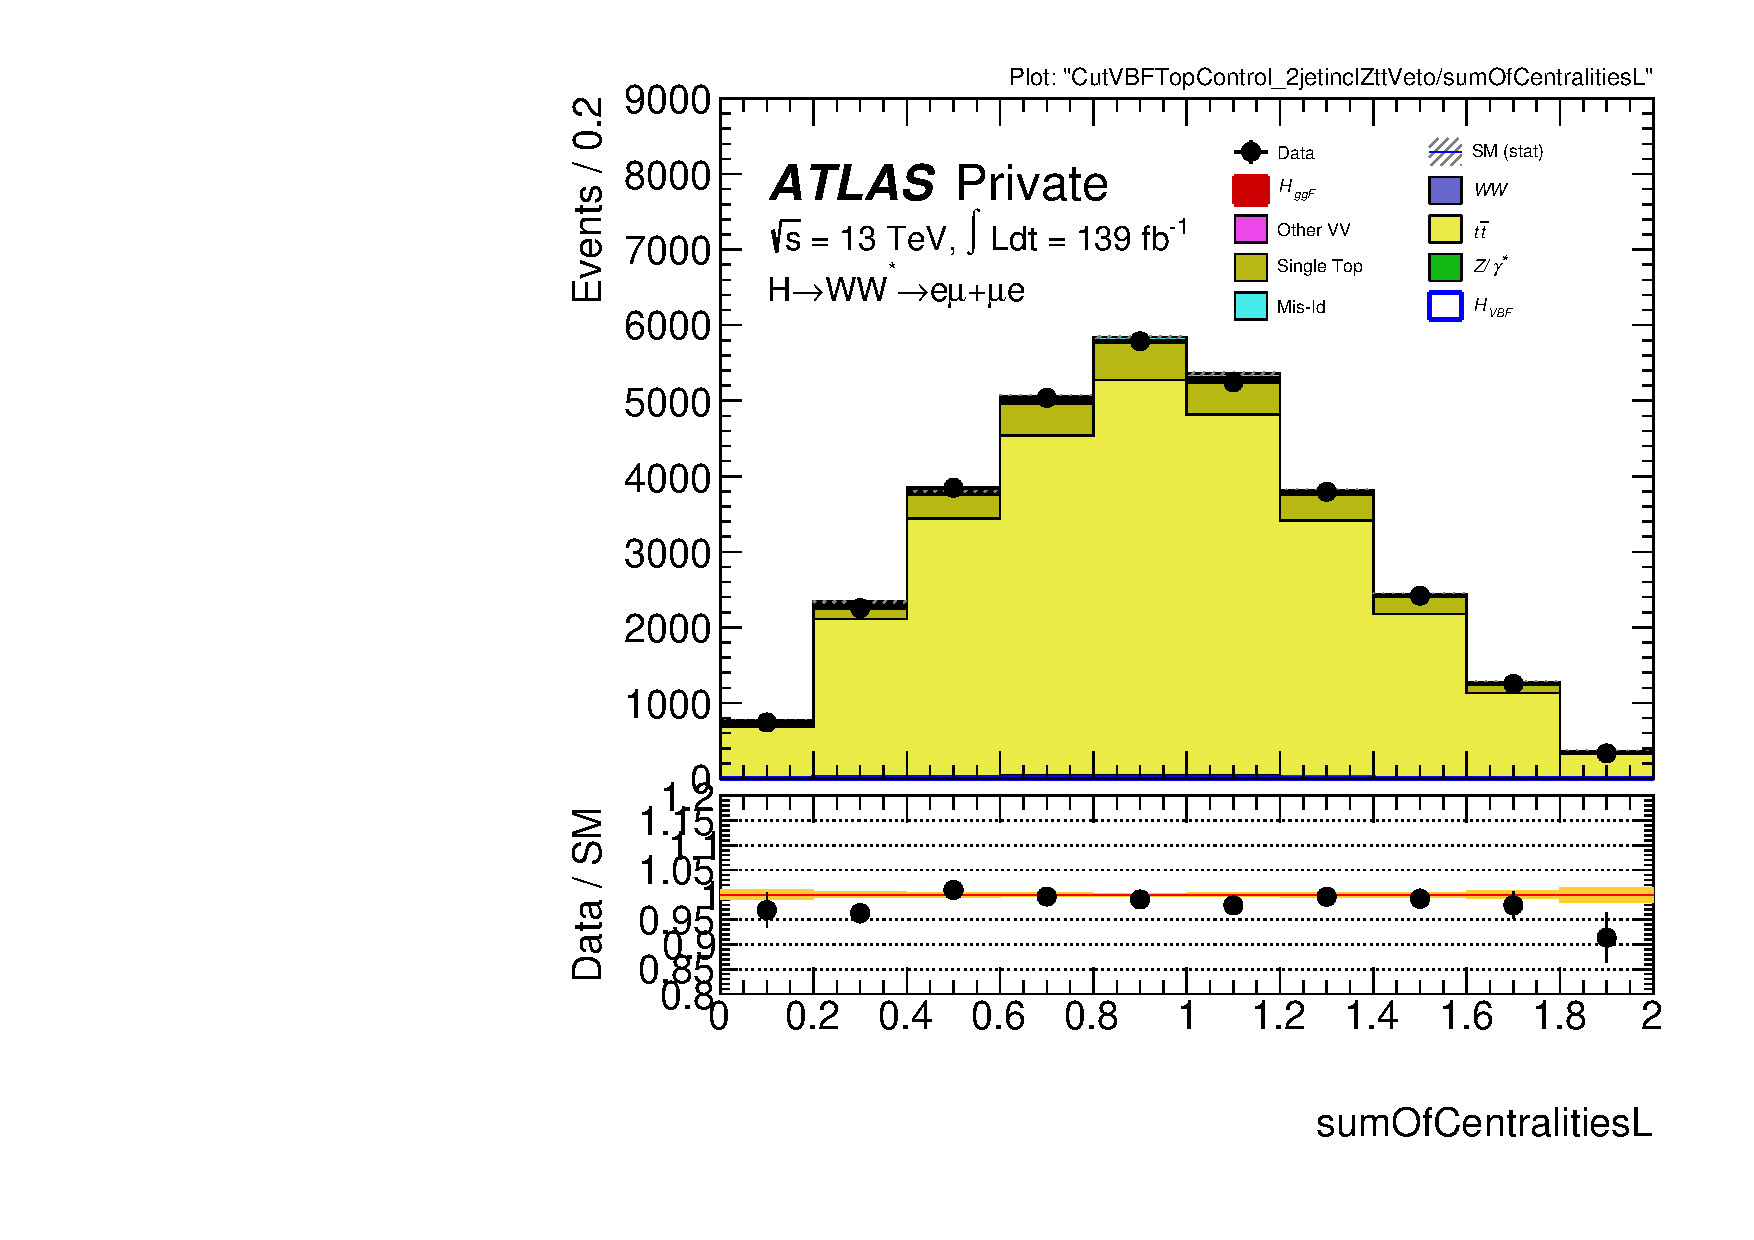
\includegraphics[width=0.3\textwidth]{Pictures/run2-emme-CutVBFTopControl_2jetinclZttVeto-sumOfCentralitiesL-lin.pdf}
  }\hfill
%  \subfloat[$m_{jj}$]{
%      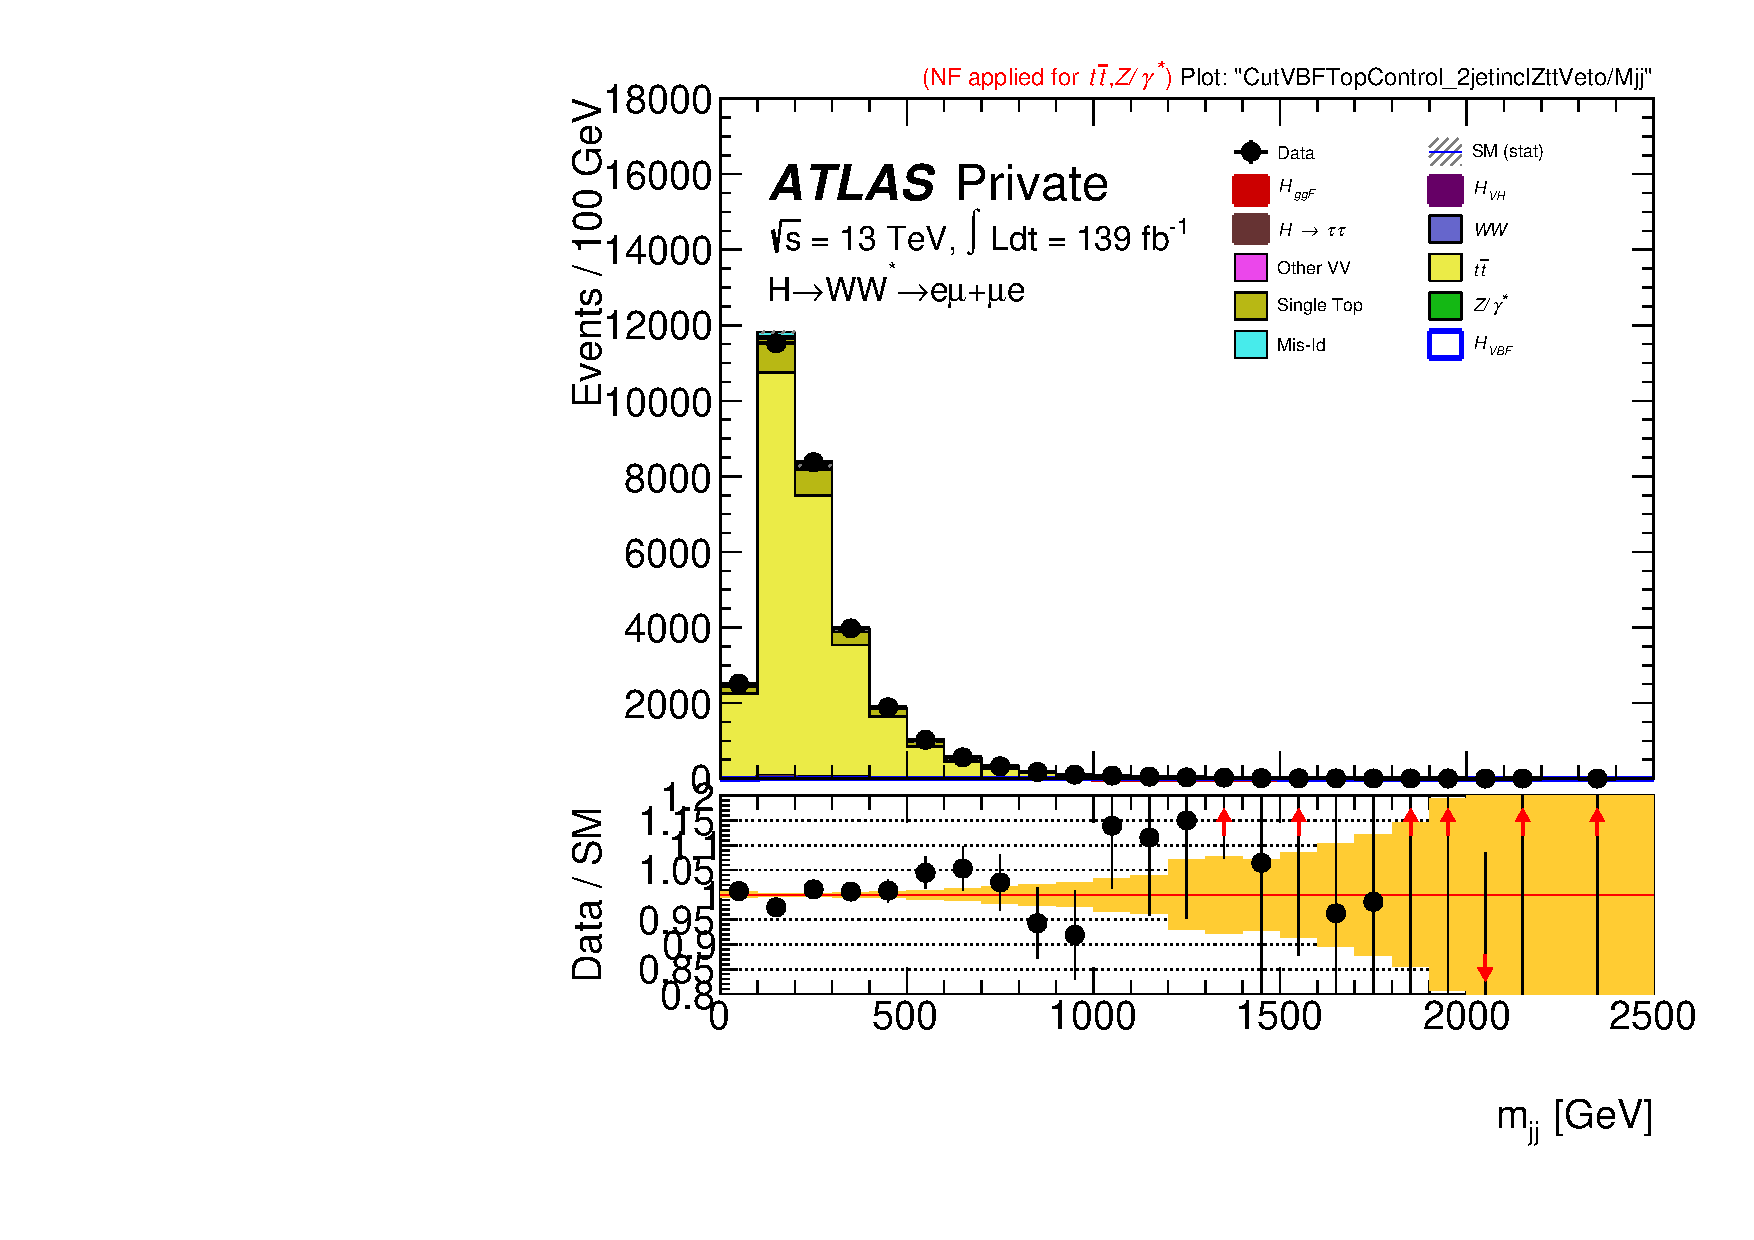
\includegraphics[width=0.3\textwidth]{Pictures/run2-emme-CutVBFTopControl_2jetinclZttVeto-Mjj-lin.pdf}
%  }\hfill
  \subfloat[$M_{l0j0}$]{
      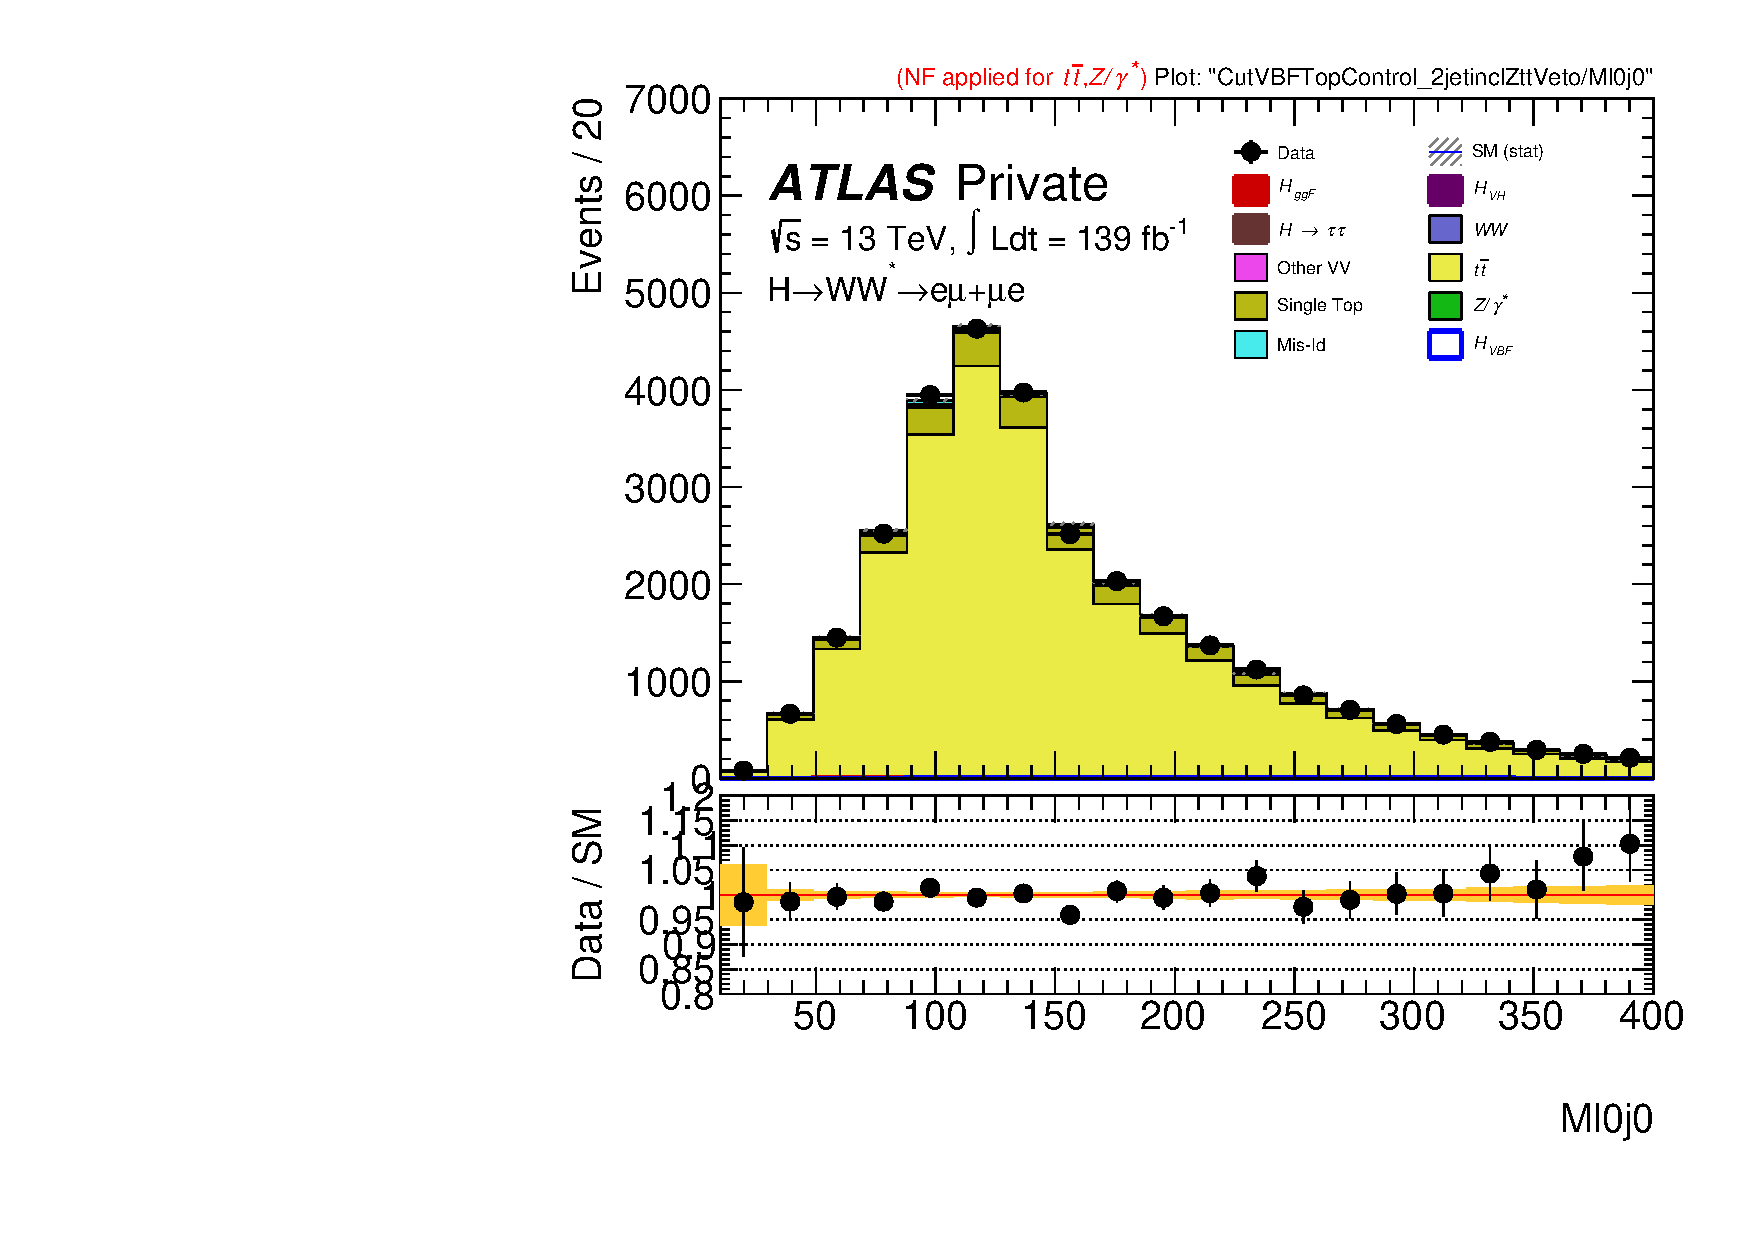
\includegraphics[width=0.3\textwidth]{Pictures/run2-emme-CutVBFTopControl_2jetinclZttVeto-Ml0j0-lin.pdf}
  }\hfill
  \subfloat[$M_{l1j1}$]{
      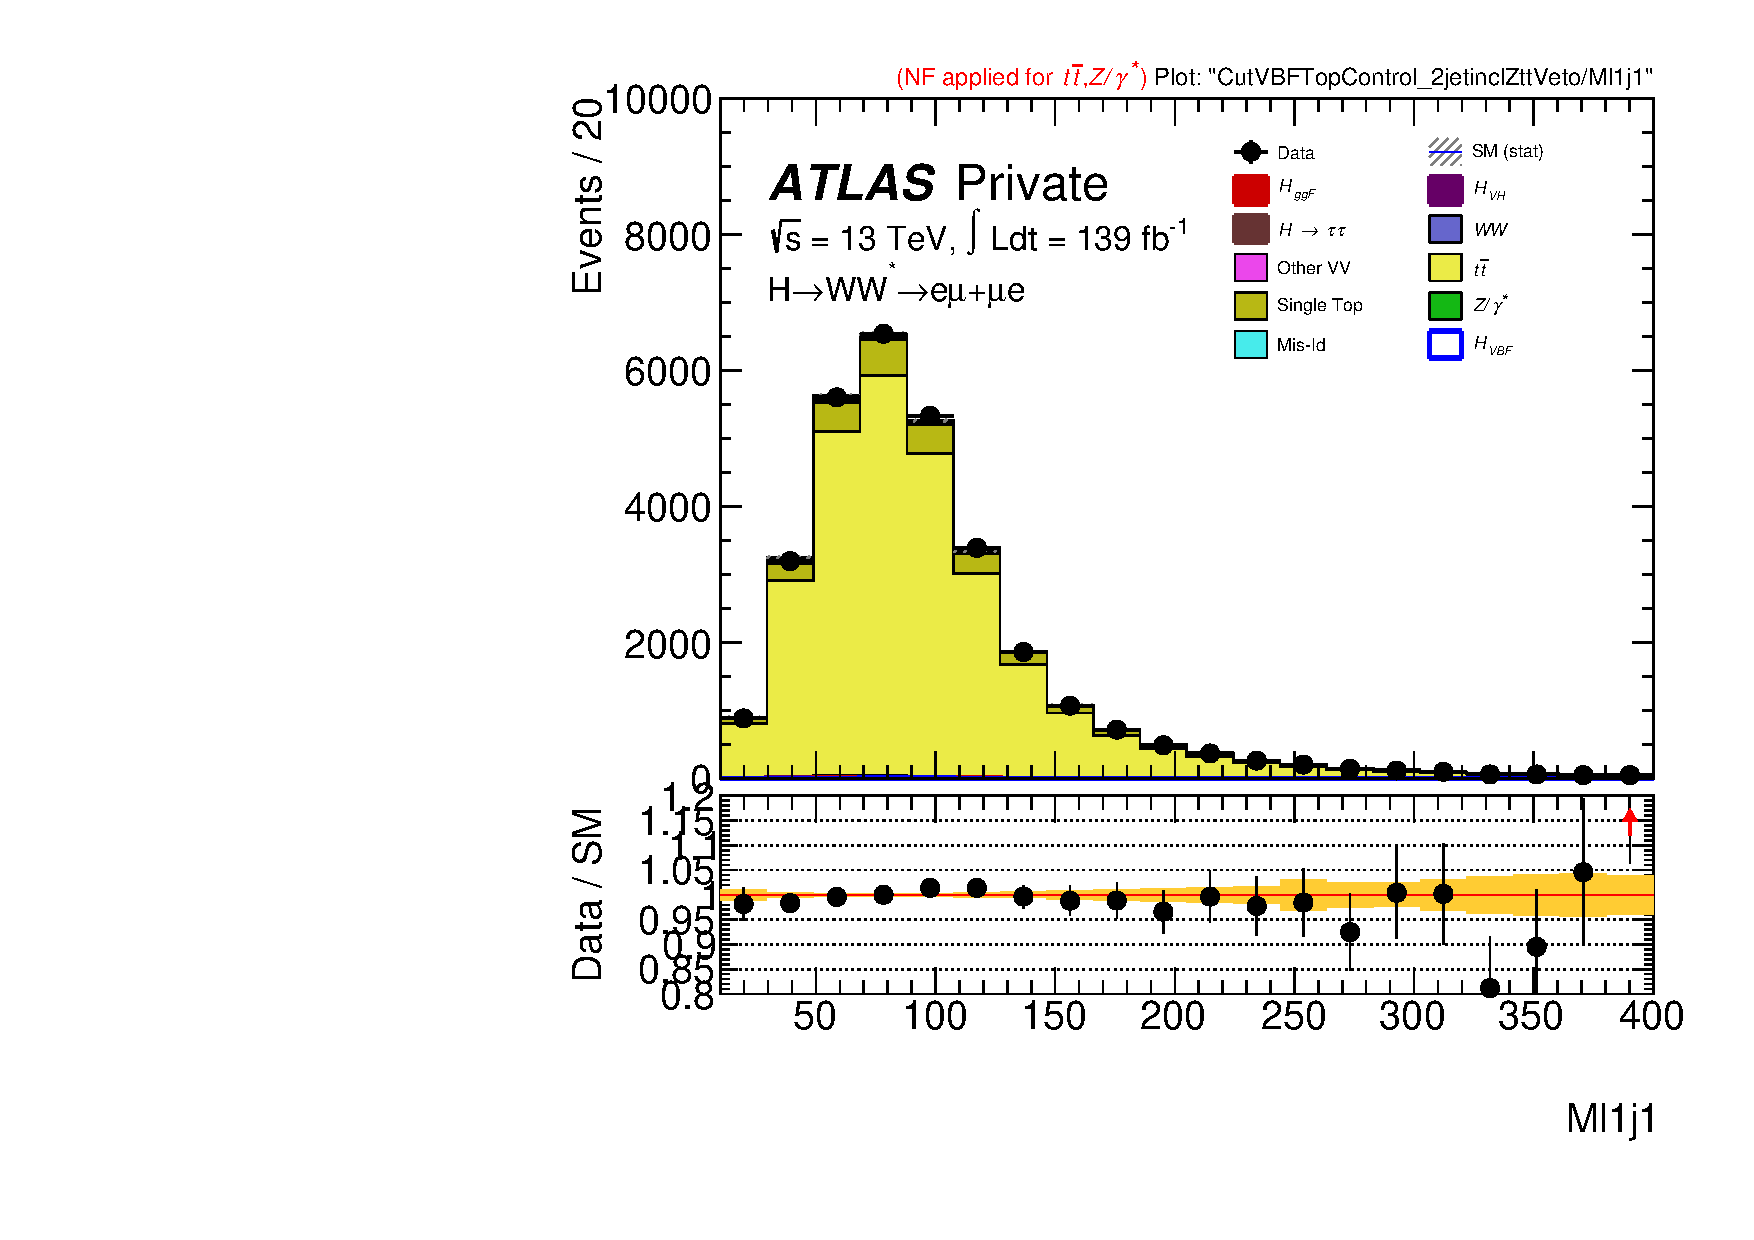
\includegraphics[width=0.3\textwidth]{Pictures/run2-emme-CutVBFTopControl_2jetinclZttVeto-Ml1j1-lin.pdf}
  }\hfill
  \subfloat[$\Delta\Phi_{jj}$]{
      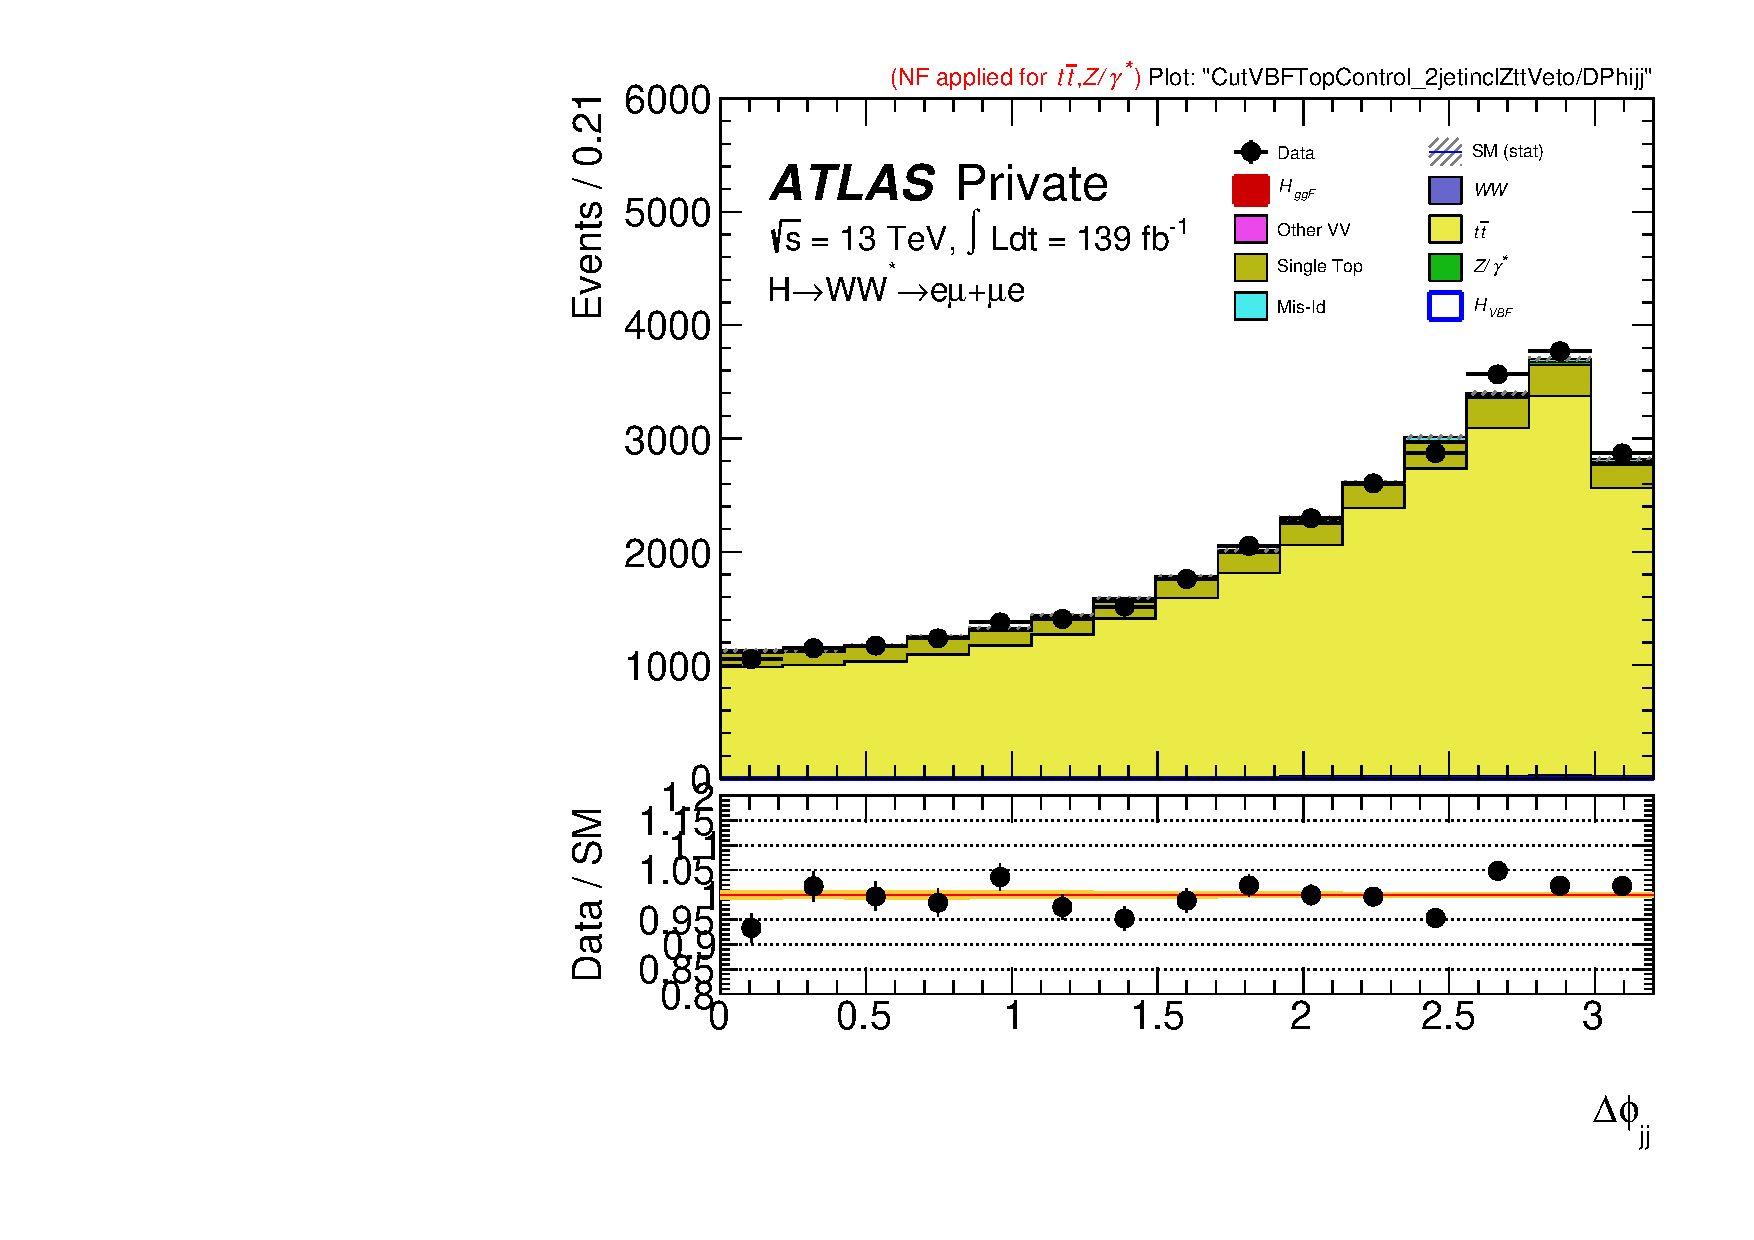
\includegraphics[width=0.3\textwidth]{Pictures/run2-emme-CutVBFTopControl_2jetinclZttVeto-DPhijj-lin.pdf}
  }\hfill
  \subfloat[$p_T^{tot}$]{
      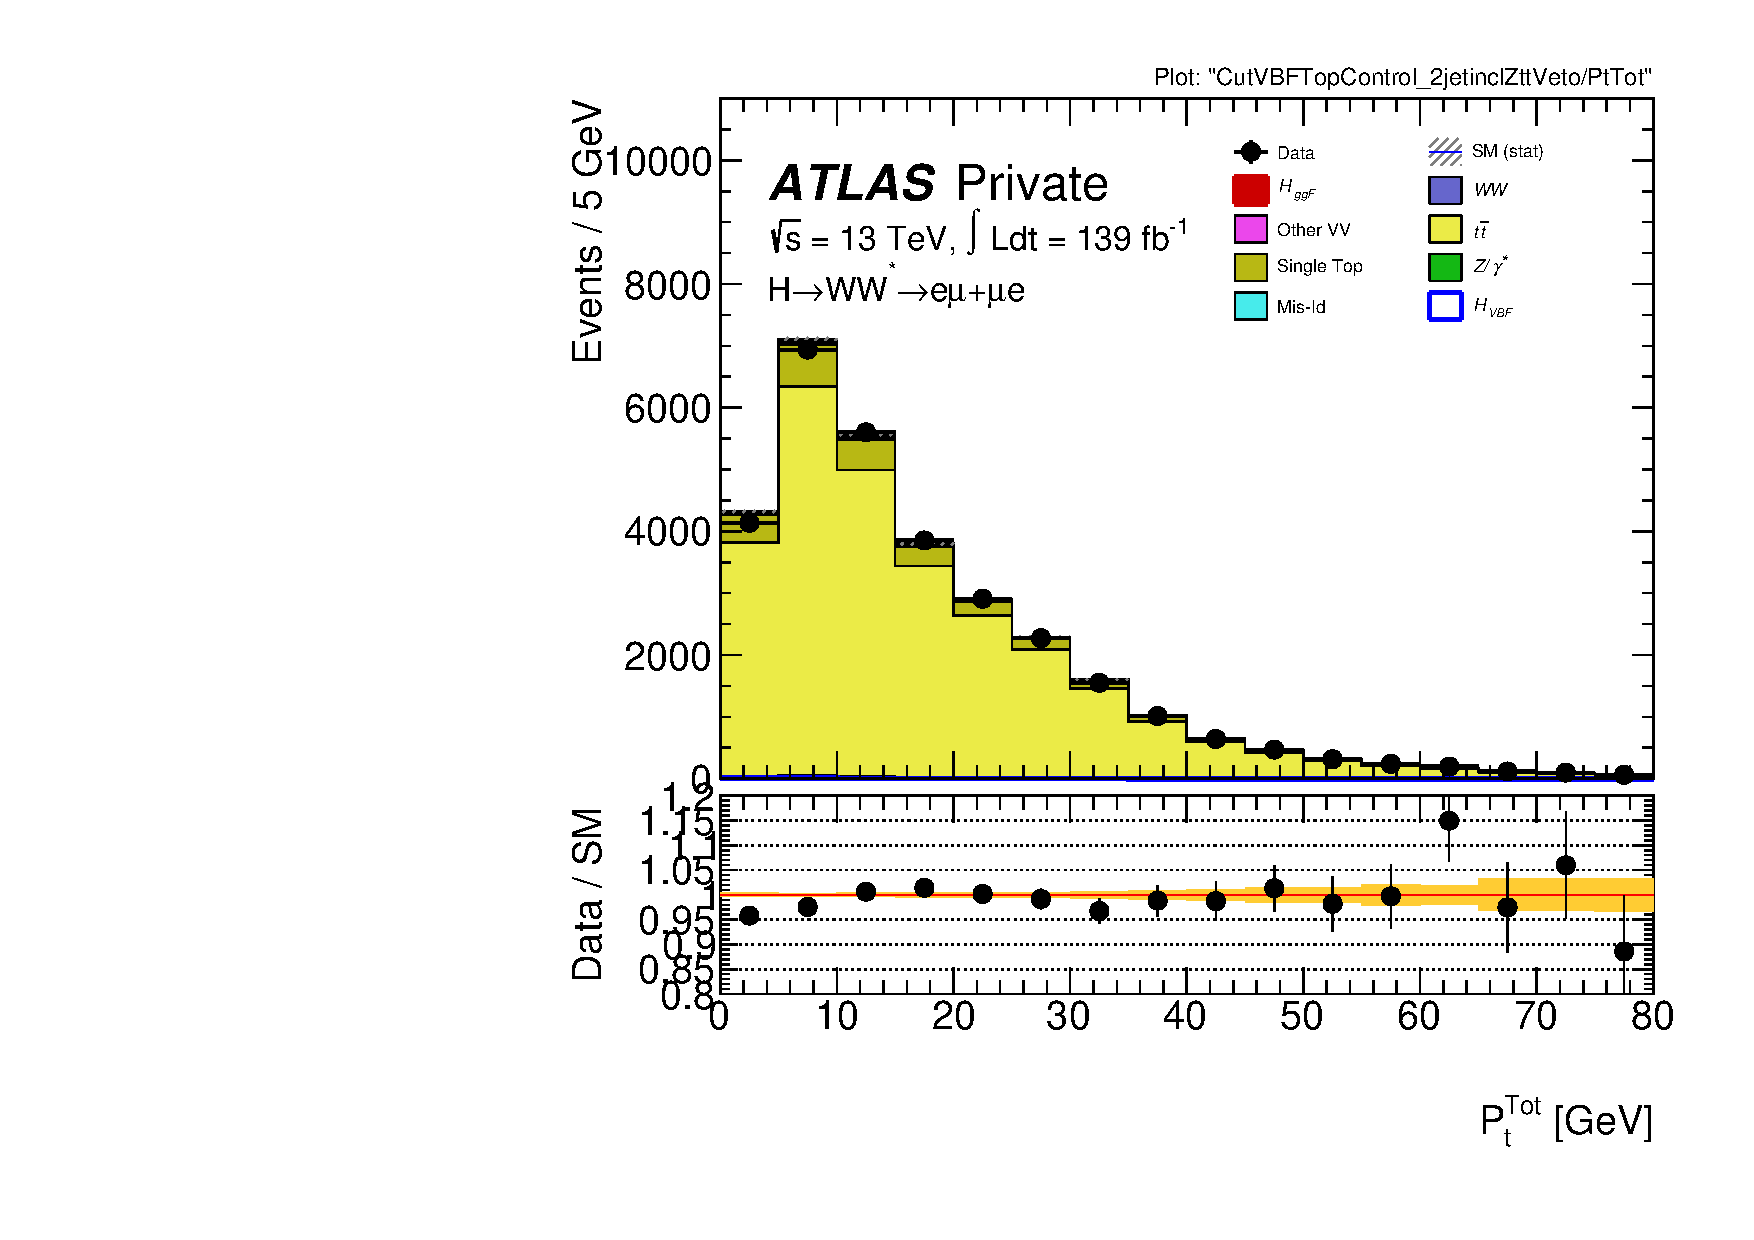
\includegraphics[width=0.3\textwidth]{Pictures/run2-emme-CutVBFTopControl_2jetinclZttVeto-PtTot-lin.pdf}
  }\hfill
  \subfloat[$m_T$]{
      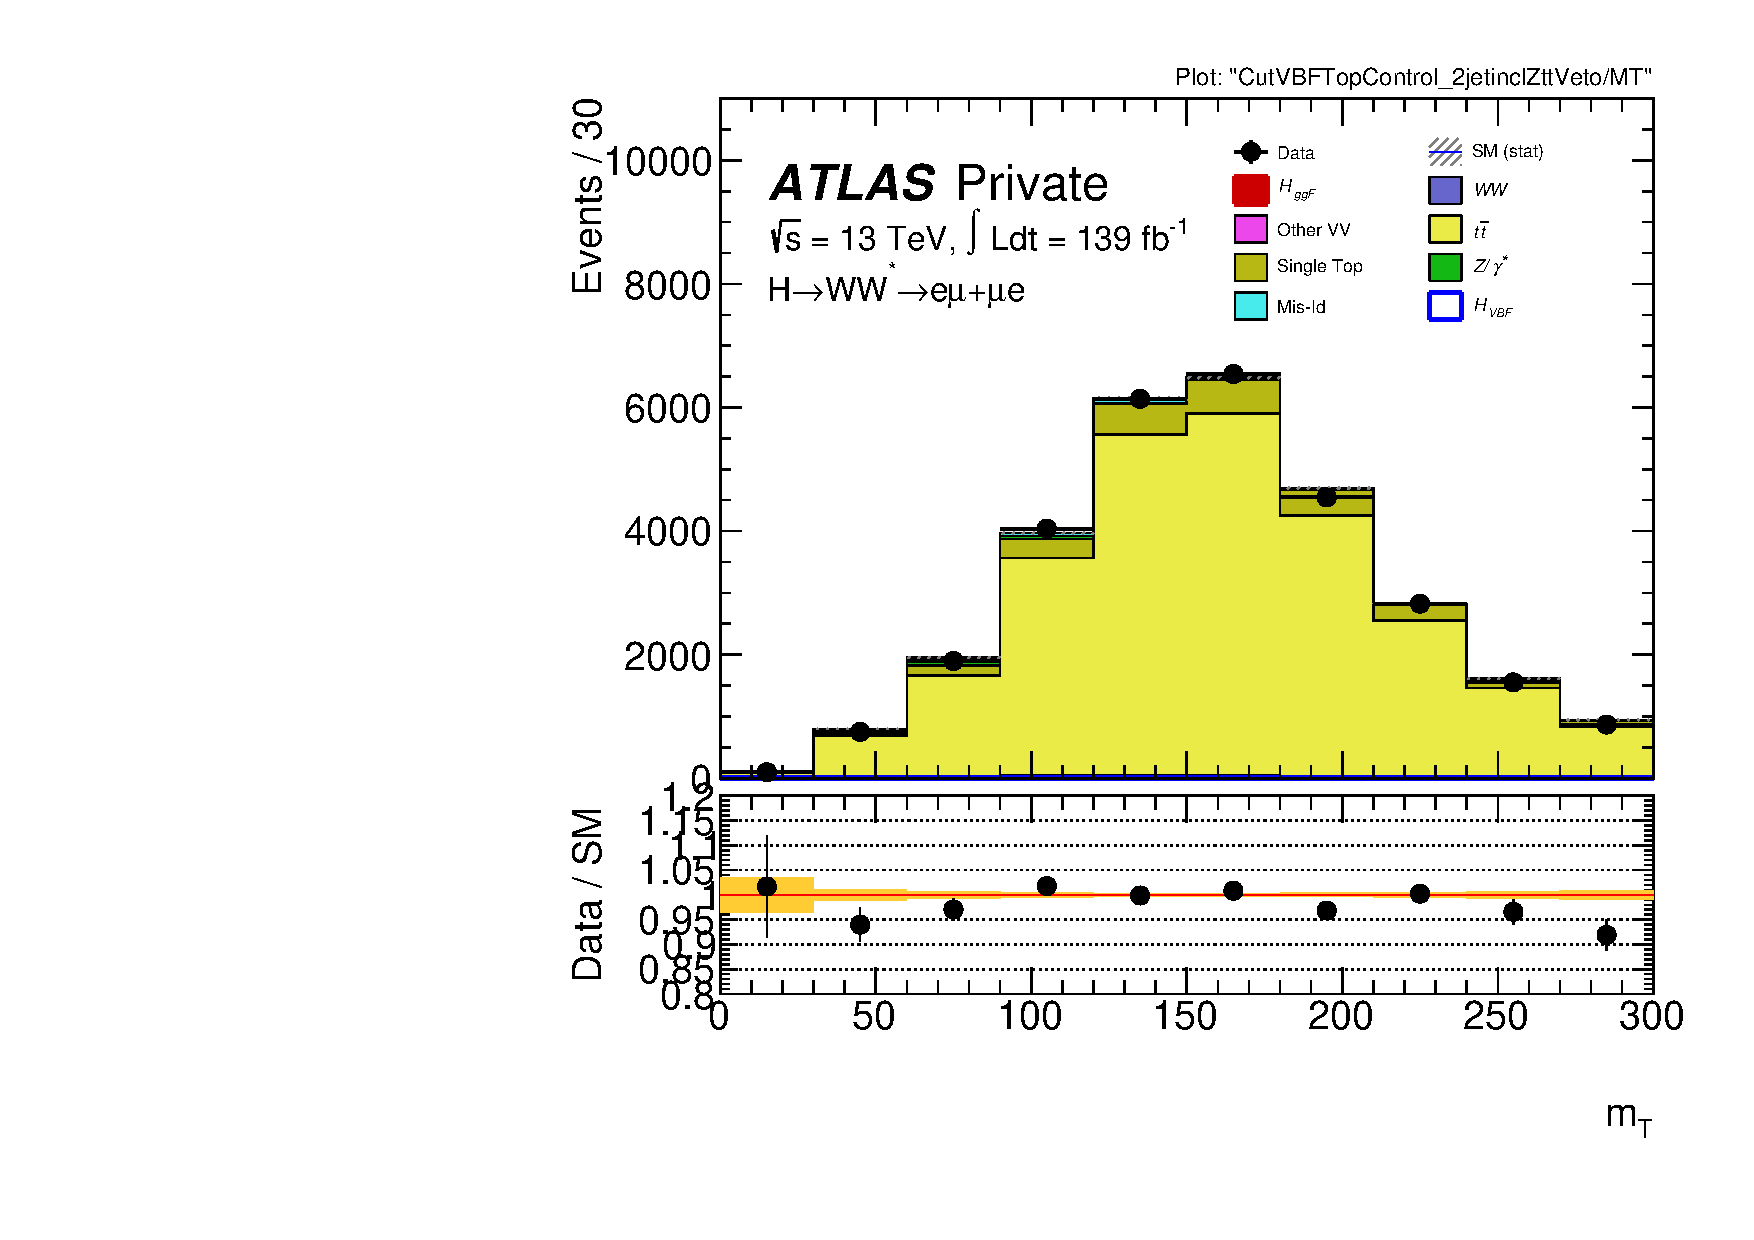
\includegraphics[width=0.3\textwidth]{Pictures/run2-emme-CutVBFTopControl_2jetinclZttVeto-MT-lin.pdf}
  }%hfill
% \subfloat[$\ensuremath{E_{\text{T}}^{\text{miss}}}$]{
%     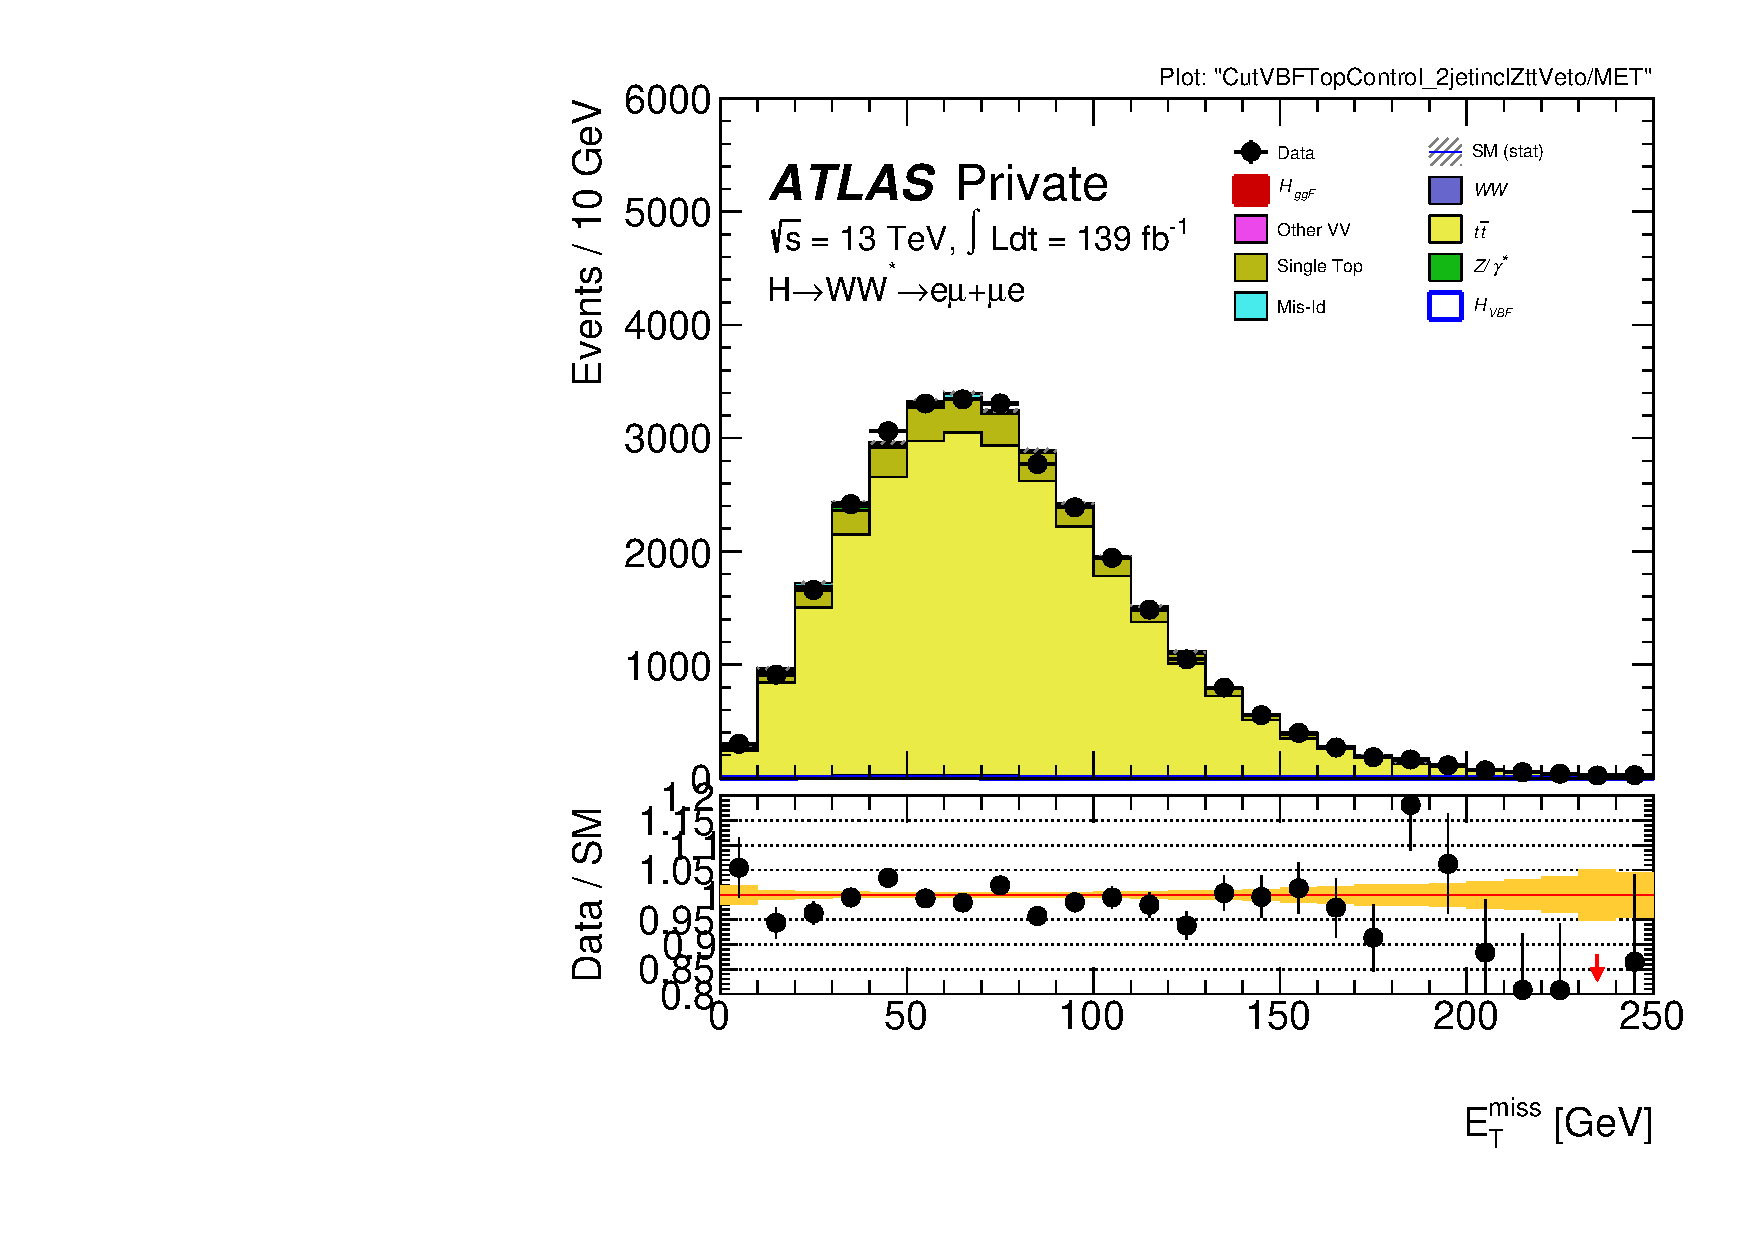
\includegraphics[width=0.3\textwidth]{Pictures/run2-emme-CutVBFTopControl_2jetinclZttVeto-MET-lin.pdf}
% }%\hfill 
{\caption{Distributions of $m_{\ell\ell}$, $\Delta Y_{\ell\ell}$, $\Delta Y_{jj}$, $\sum$ centralities, $M_{l0j0}$, $M_{l1j1}$, $\Delta\Phi_{jj}$, $p_T^{tot}$, and $m_T$ in the top validation region.
\label{fig:TopCR3}}}
\end{figure}

\subsubsection{Top and $WW$ BDT discriminant (against all other samples)}

This BDT is trained using $e\mu+\mu e$ events after the VBF selection and all signal regions cuts so that the phase space in which we train the BDT is exactly the same as the one where we apply it in the final fit. The training includes top and $WW$ trained against weighted samples of VBF, ggF, $Z+$jets, and $V\gamma$ events. The MC statistics used in the training are half those available after all signal region cuts and the other half are later used to test the training. This corresponds to $\approx$ 90,000 un-weighted $WW$ and top events and $\approx$ 115,000 raw VBF, ggF, $Z+$jets and $V\gamma$ events. This training includes MC weights on events to best account for overall event distributions and there are $\approx$ 2000 total weighted top and $WW$ events used in the training and $\approx$ 550 weighted other events. 

The TMVA BDTG interface is used to train and test the BDT. The optimal parameters were found through a scan of reasonable values and the final set is summarized in Table~\ref{tab:TopBDTparameters}.
\begin{table}[h!]
\centering
\begin{tabular}{|l|c|}
\hline
Parameter                                    & Value     \\
\hline
Boosting algorithm                           &  Gradient  \\
Maximum tree depth                           &  22       \\
Number of trees                              &  200     \\
Minimum number of events requires per mode   &  5\%      \\
Number of cuts                               &  7        \\
\hline
\end{tabular}
\caption{BDT parameters used for the top + $WW$ vs. other backgrounds training.} 
\label{tab:TopBDTparameters}
\end{table}

This BDT utilizes a range of lepton and jet kinematic variables (8) to distinguish between signal and background events. These include $\Delta Y_{jj}$, the combination of lepton/jet masses $M_{l0j0}$ for leading and subleading leptons and jets, $\Delta \Phi_{\ell\ell}$, $m_T$, $\eta_{j0}$, $\eta_{j1}$, $\Delta \Phi_{jj}$, and $\sum$ centralities (L). While a larger variety of variables have been tested, these demonstrated the highest discrimination between top/$WW$ events and other samples. Plots shown in \ref{fig:TopBDTinput} and \ref{fig:TopcorrSB} demonstrate the input distributions used to train the BDT and their correlations.
\begin{figure}[!htbp]
    \centering
    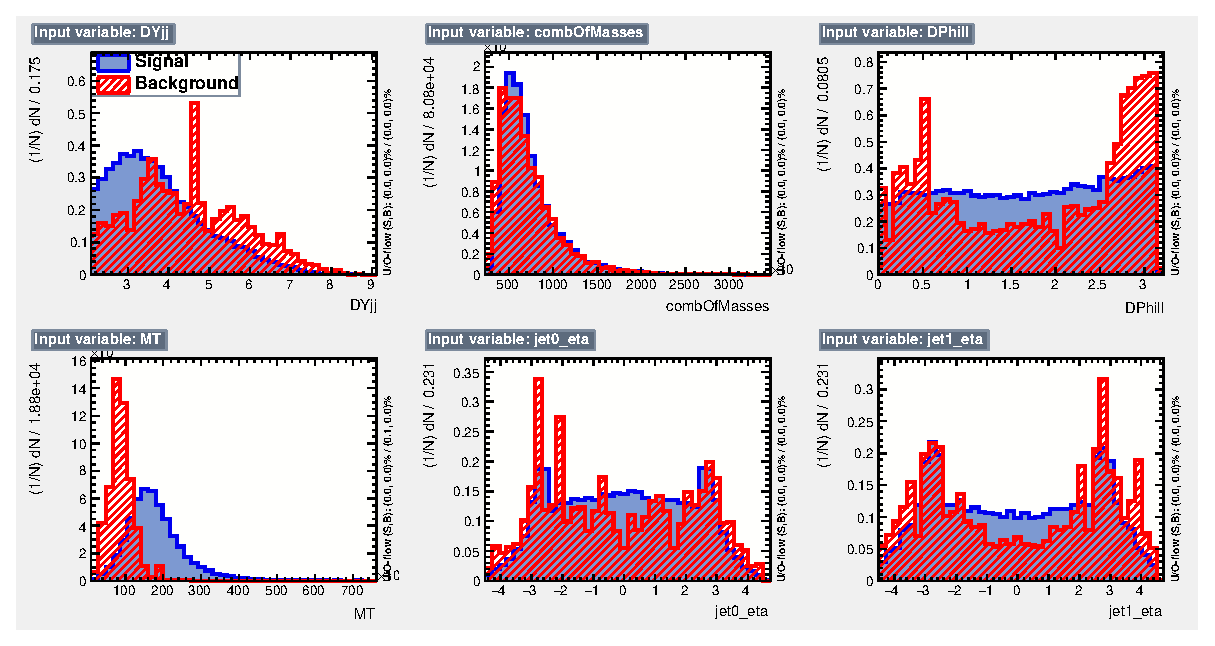
\includegraphics[width=0.45\linewidth]{Pictures/Top+WWvsEverything/variables_id_c1.eps}
    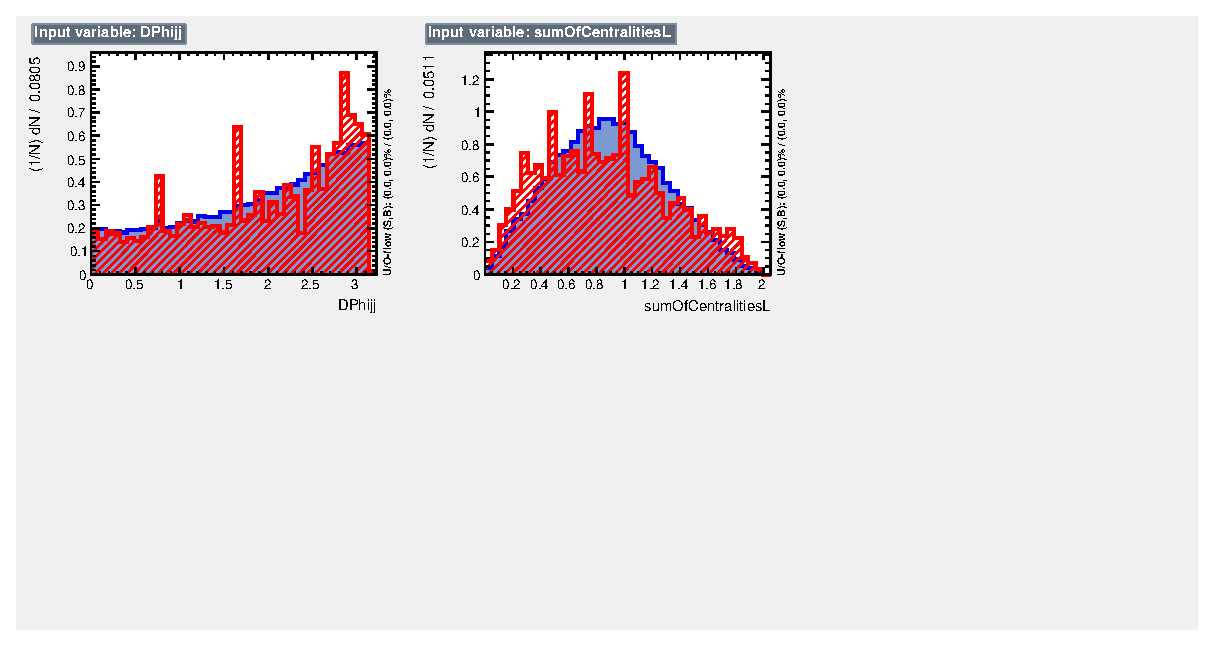
\includegraphics[width=0.45\linewidth]{Pictures/Top+WWvsEverything/variables_id_c2.eps}
    \caption{Distributions of input variables to top+$WW$ vs. other samples BDT. Samples are weighted and normalized to even numbers of background and signal events. Signal represents top+$WW$ and background all other samples.*}.
    \label{fig:TopBDTinput}
\end{figure}
\begin{figure}[!htbp]
\centering
  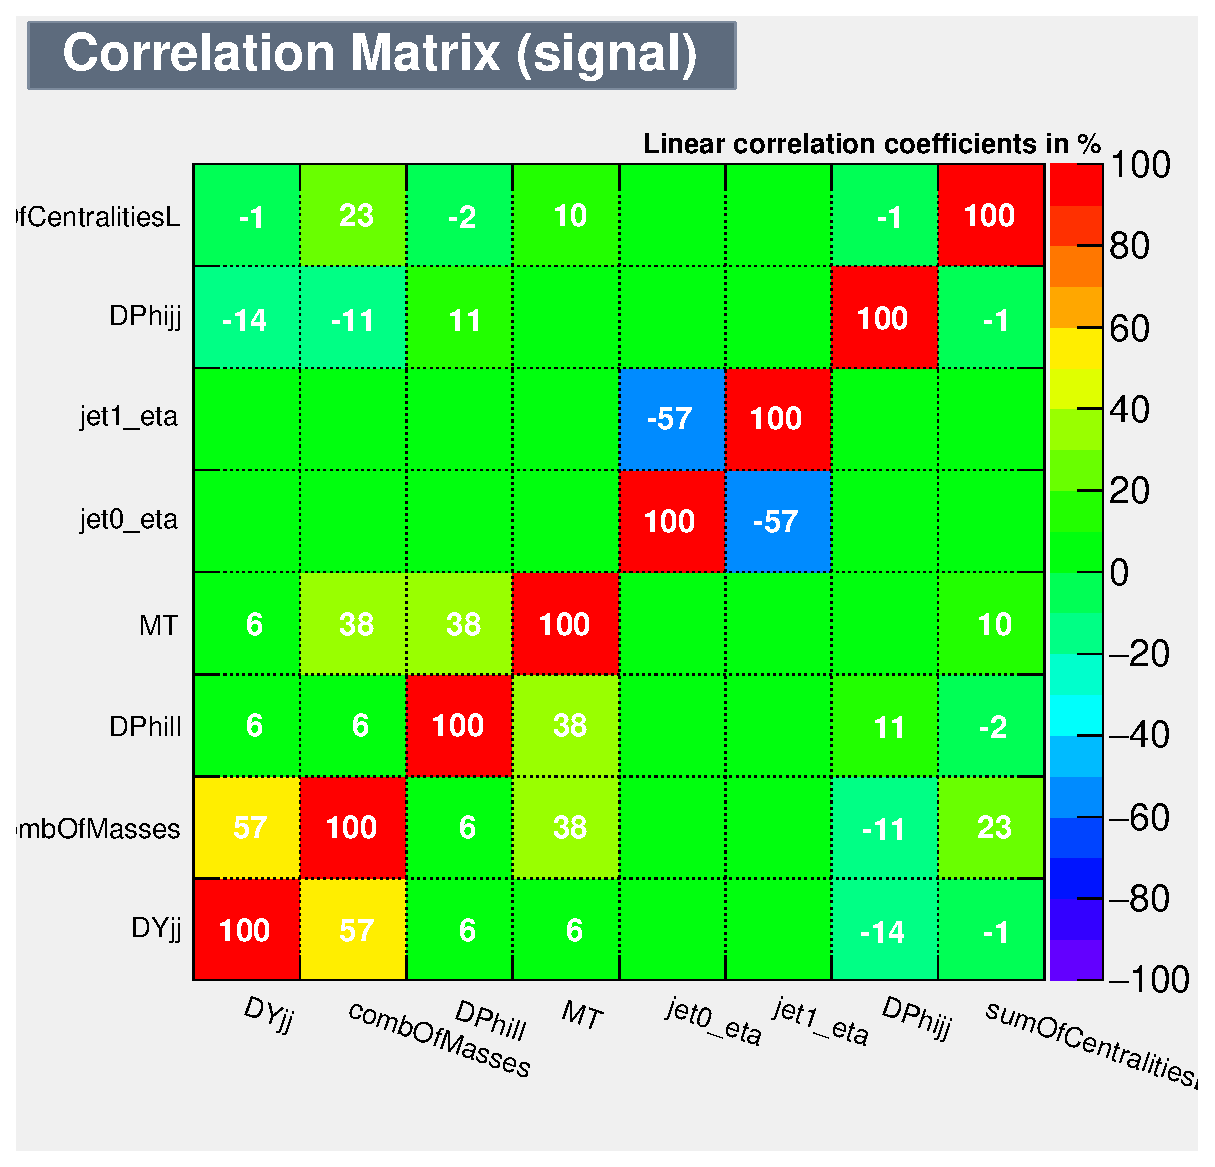
\includegraphics[width=.3\linewidth]{Pictures/Top+WWvsEverything/CorrelationMatrixS.eps}
  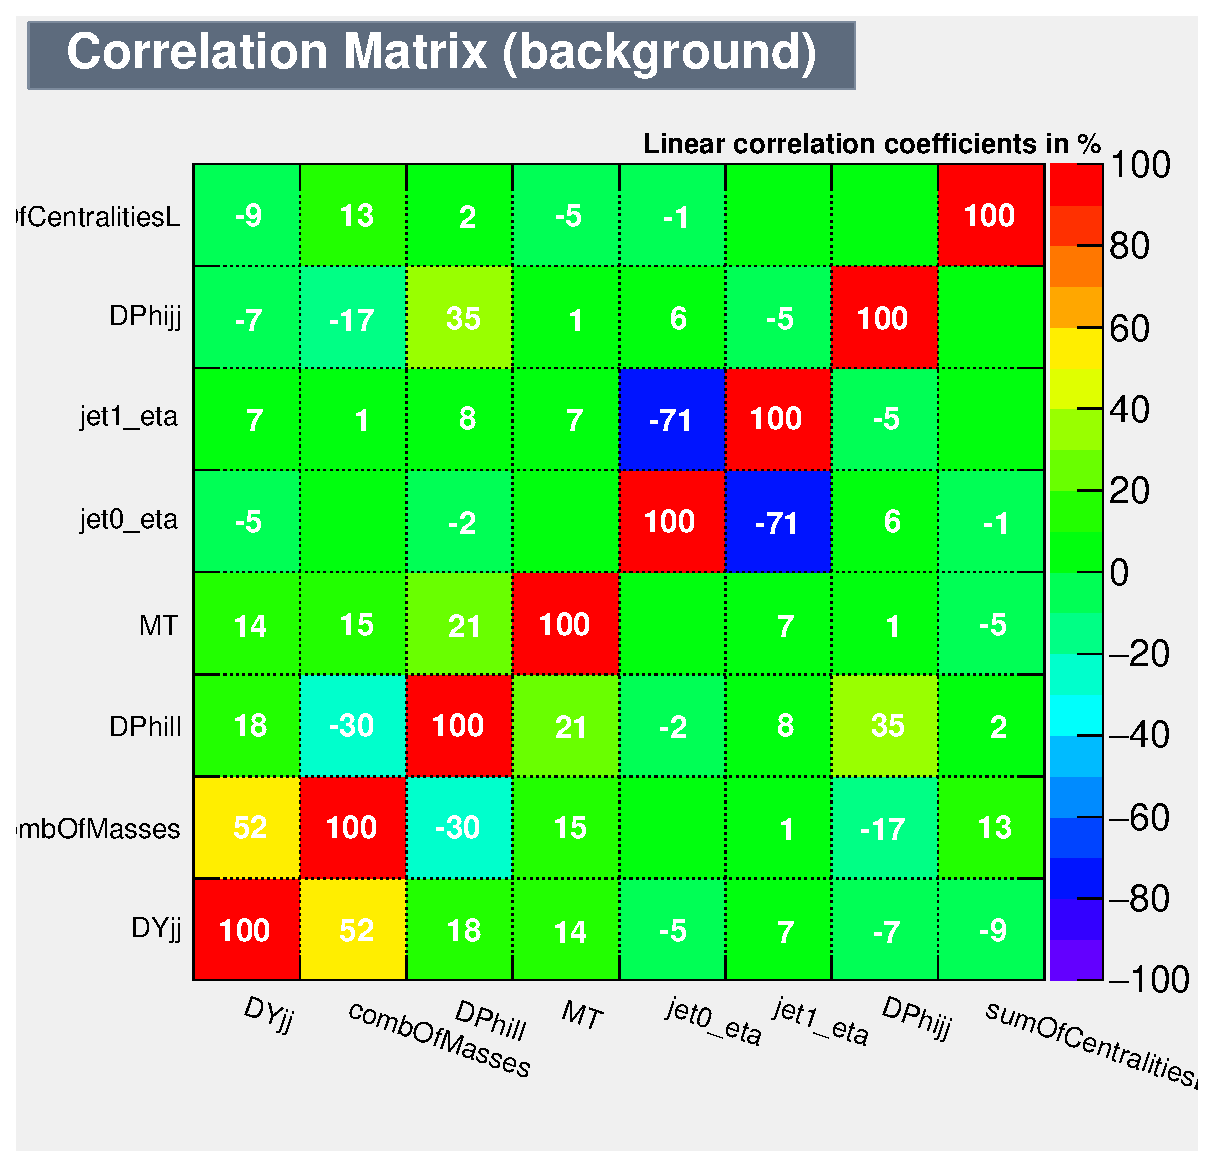
\includegraphics[width=.3\linewidth]{Pictures/Top+WWvsEverything/CorrelationMatrixB.eps}
\caption{Correlations of input variables to top +$WW$ vs other samples BDT. Signal represents top+$WW$ and background other samples.*}
\label{fig:TopcorrSB}
\end{figure}
The BDT training successfully separates top/$WW$ background and other samples (ggF, VBF, $Z+$jets, and $V\gamma$). In order to quantify the discrimination we use the integrated-ROC calculated through TMVA for weighted normalized samples and find an optimal value of 0.920. Comparisons between the test and training show that the BDT is un-biased- differences between testing and training samples would imply overtraining, or the BDT using to many parameters on too few events. For signal and background we find KS-test values of 0.107 and 0.154, and so no evidence of over-training. We can visualize the BDT output variable both on weighted normalized samples and on samples with full event weights applied. The following plot shows BDT results applied to all samples.

\begin{figure}[!htbp]
\centering
  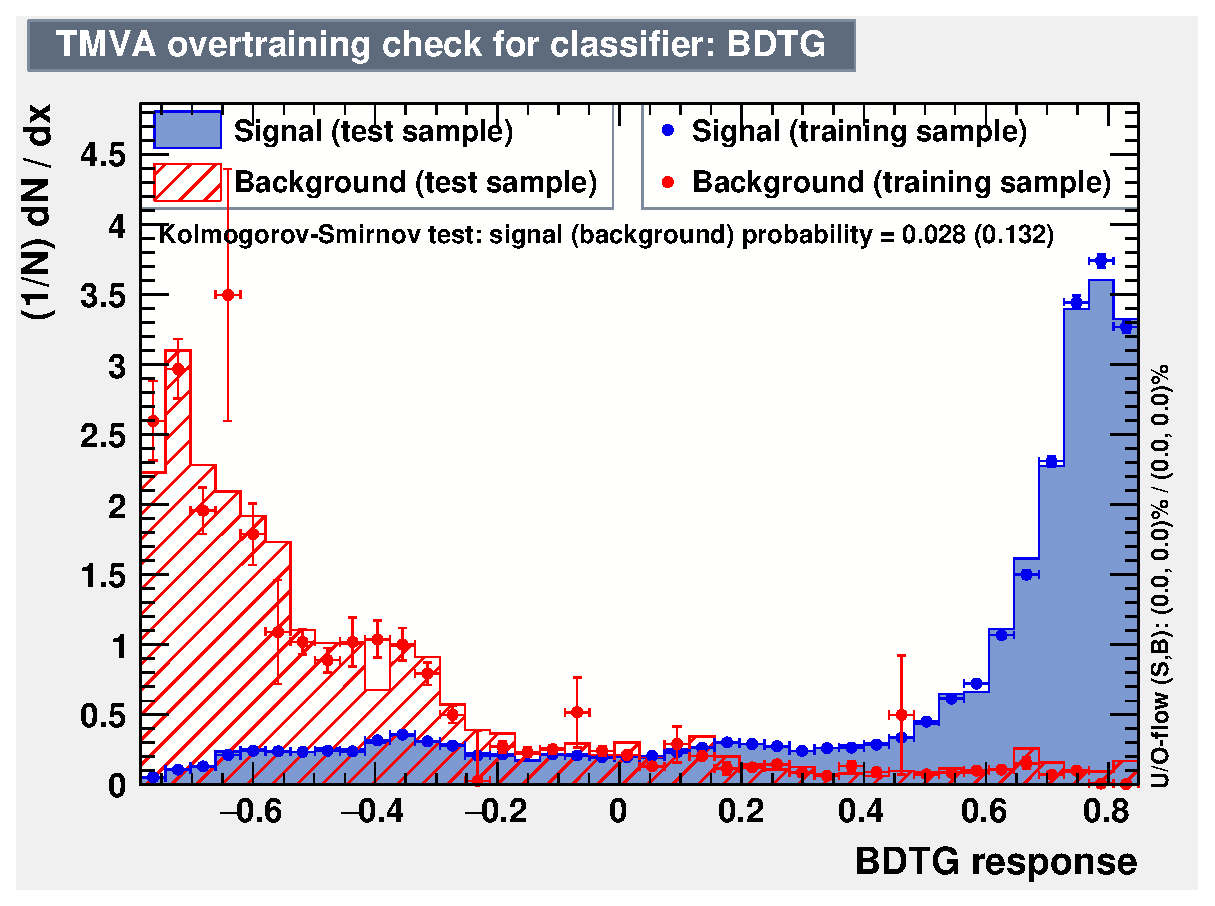
\includegraphics[width=.4\linewidth]{Pictures/Top+WWvsEverything/overtrain_BDTG.eps}
  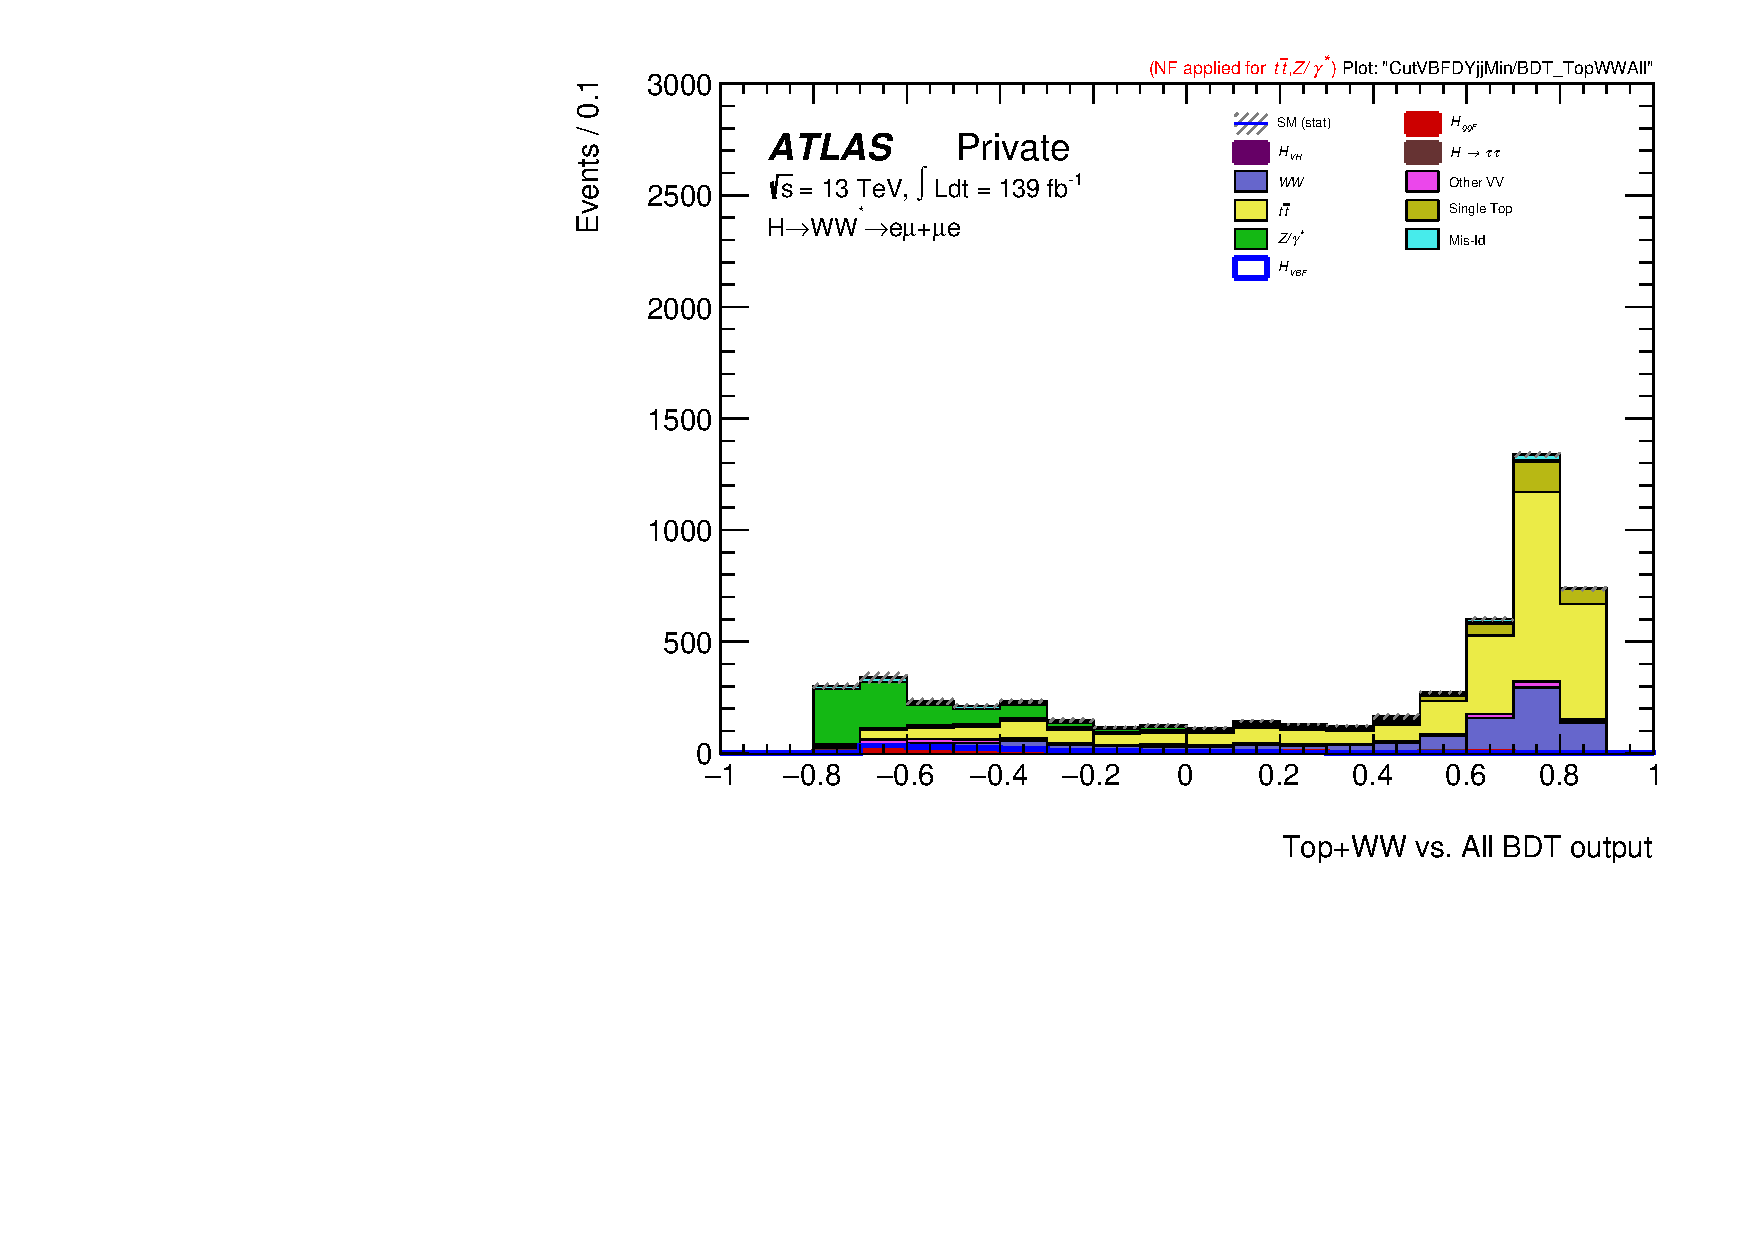
\includegraphics[width=.45\linewidth]{Pictures/run2-emme-CutVBFDYjjMin-BDT_TopWWAll-lin.pdf}
\caption{Weighted, normalized samples of top$+WW$ samples (signal) and other samples (background) plotted over BDT output distribution on left, overlaid testing and training samples shown. Right, full weighted samples of all signal and background events plotted over BDT output distribution after signal region selection. Data is blinded here*}
\label{fig:TopBDTresult}
\end{figure}

We aim to fit this distribution in the signal region with high significance for top/$WW$ events in uppermost bins of the distribution. Since this BDT is trained and applied in the signal region we cannot directly test the modelling of input variables. However, modelling at the pre-selection level for each of these variables as well as in the top validation region described eariler show no evidence of mis-modelling. The binning for this discriminant used in the statistical fit and its result (using Asimov data) are shown in the final chapter. We can visualize this BDT discriminant in the top validation region to gain an idea of overall modelling (particularly of the reasonably pure top events).

\begin{figure}[!htbp]
\centering
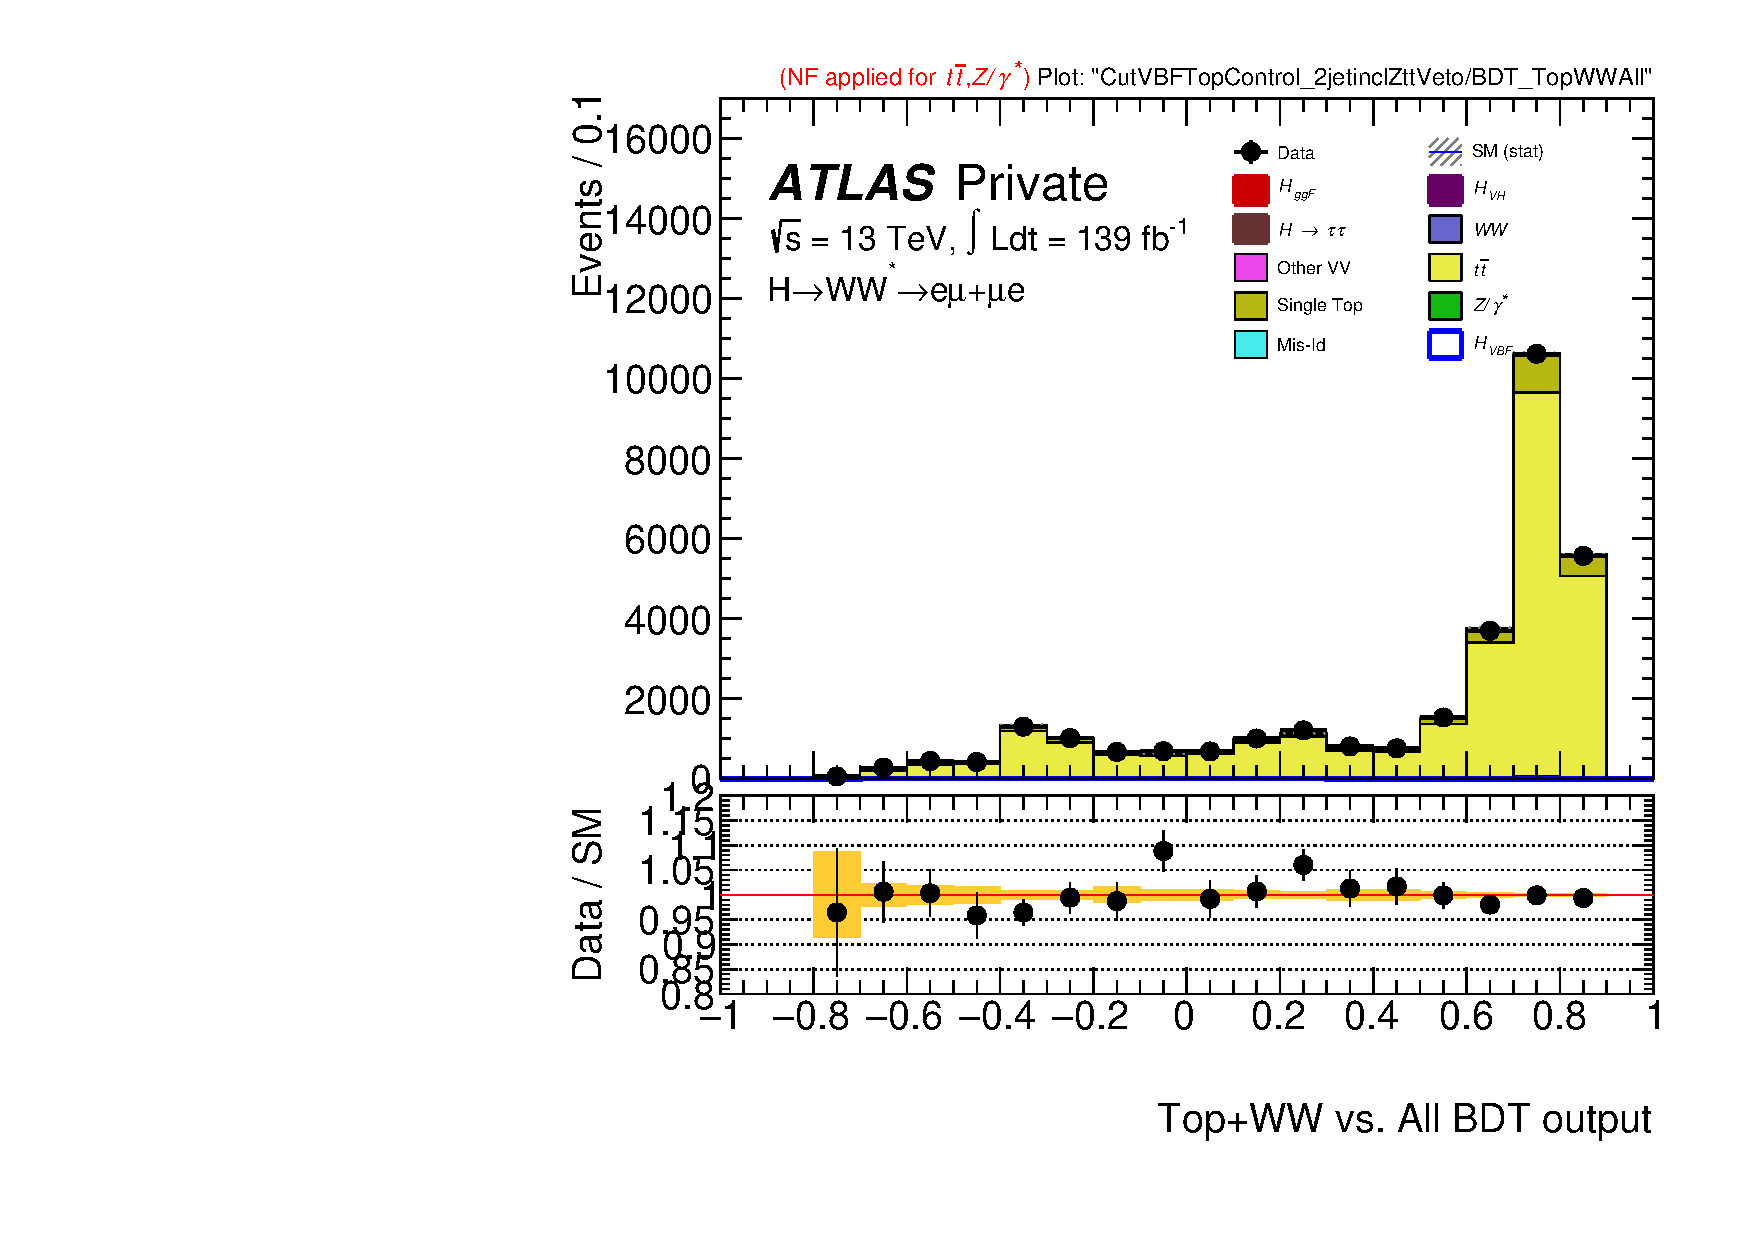
\includegraphics[width=.5\linewidth]{Pictures/run2-emme-CutVBFTopControl_2jetinclZttVeto-BDT_TopWWAll-lin.pdf}
\caption{Full weighted samples of all signal and background plotted over Top + $WW$ vs. VBF ggF + $Z+$jets +$V\gamma$ BDT output distributions in top validation region}
\label{fig:VBFTopWWBDTVR}
\end{figure}

The BDT to discriminate top$+WW$ background from VBF signal events is trained and applied in the signal region and so described in the previous chapter, but its distribution in the top validation region is also shown. 

\begin{figure}[!htbp]
\centering
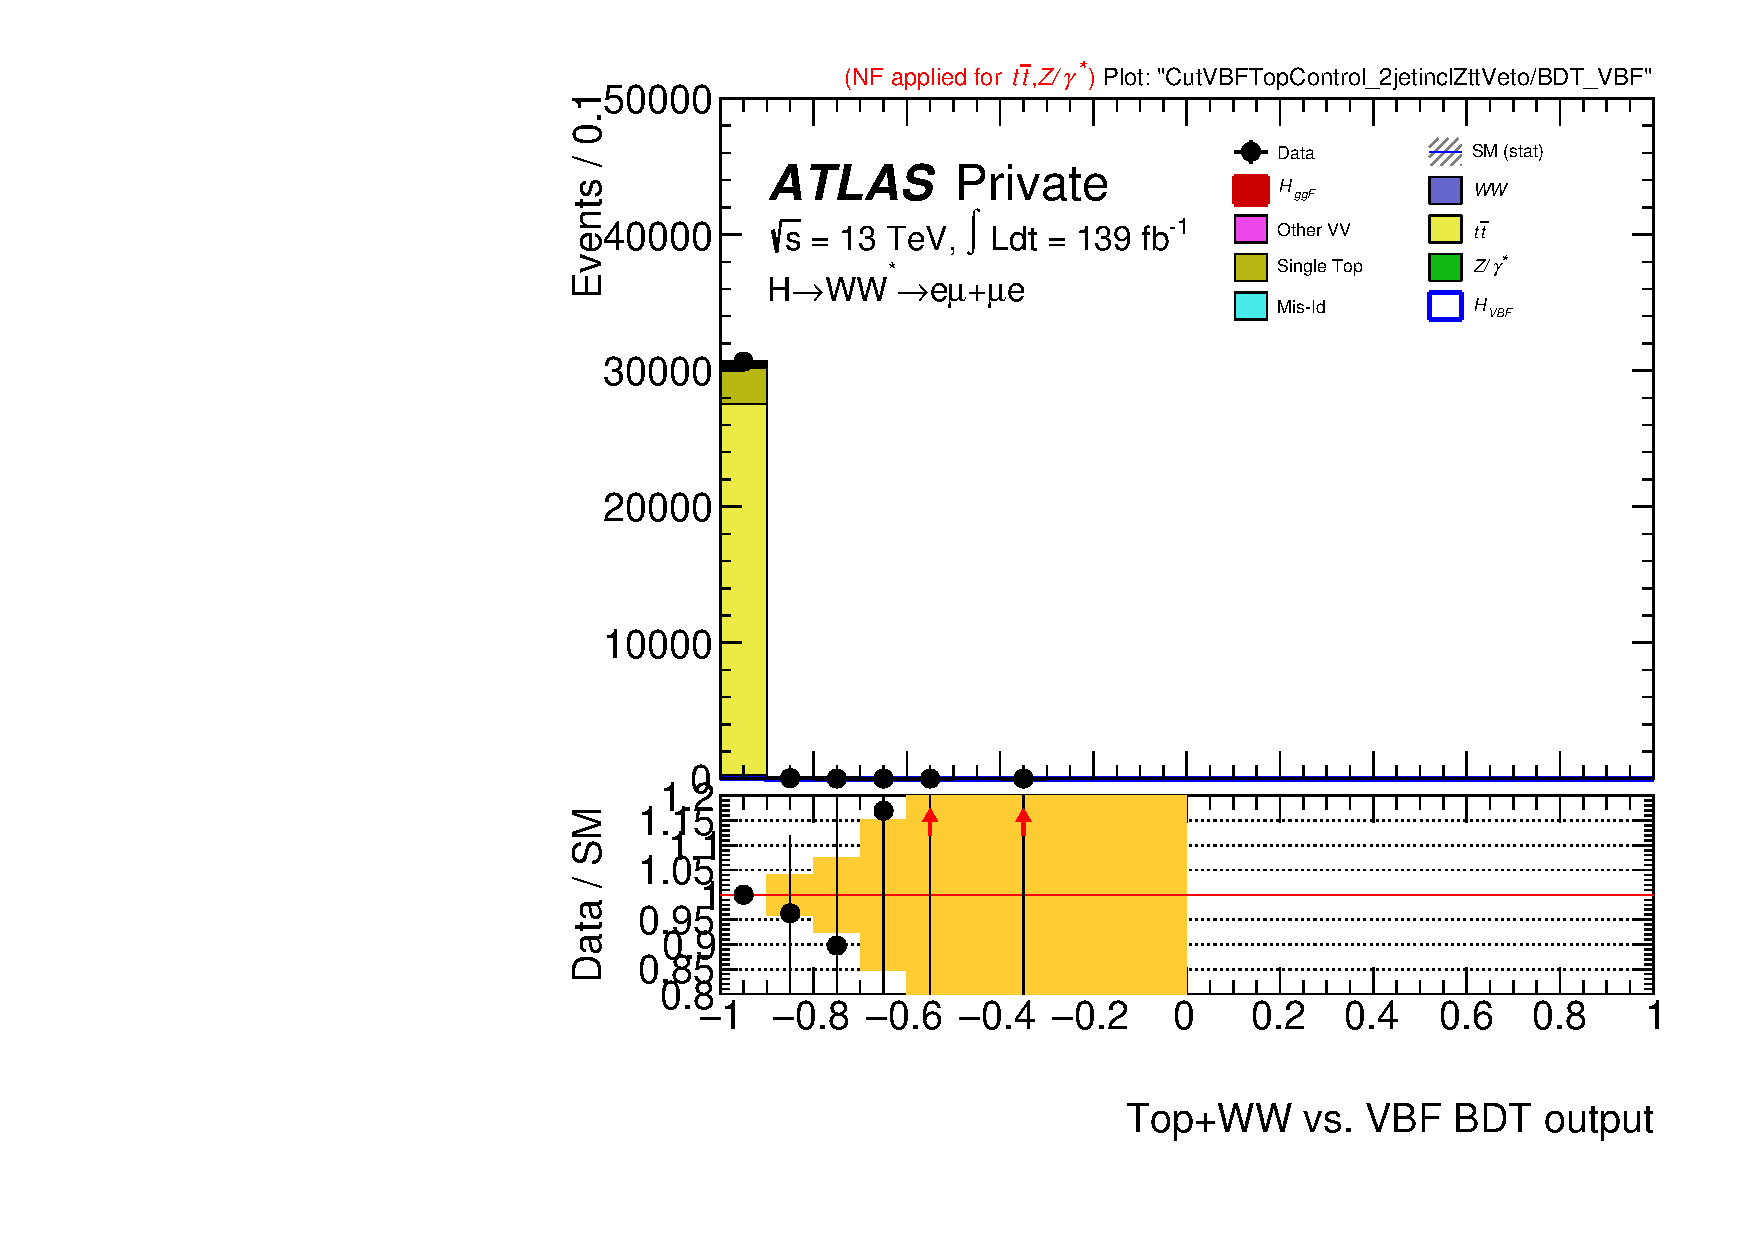
\includegraphics[width=.5\linewidth]{Pictures/run2-emme-CutVBFTopControl_2jetinclZttVeto-BDT_VBF-lin.pdf}
\caption{Full weighted samples of all signal and background plotted over Top + $WW$ vs. VBF BDT output distributions in top validation region}
\label{fig:VBFTopWWBDTVR}
\end{figure}

A designated BDT discriminates between top and WW backgrounds and is described further in the WW background section (next). However, this distribution in the top validation region with all weighted samples is shown below. to demonstrate its effect on primarily predominantly top-like events.

\begin{figure}[!htbp]
\centering
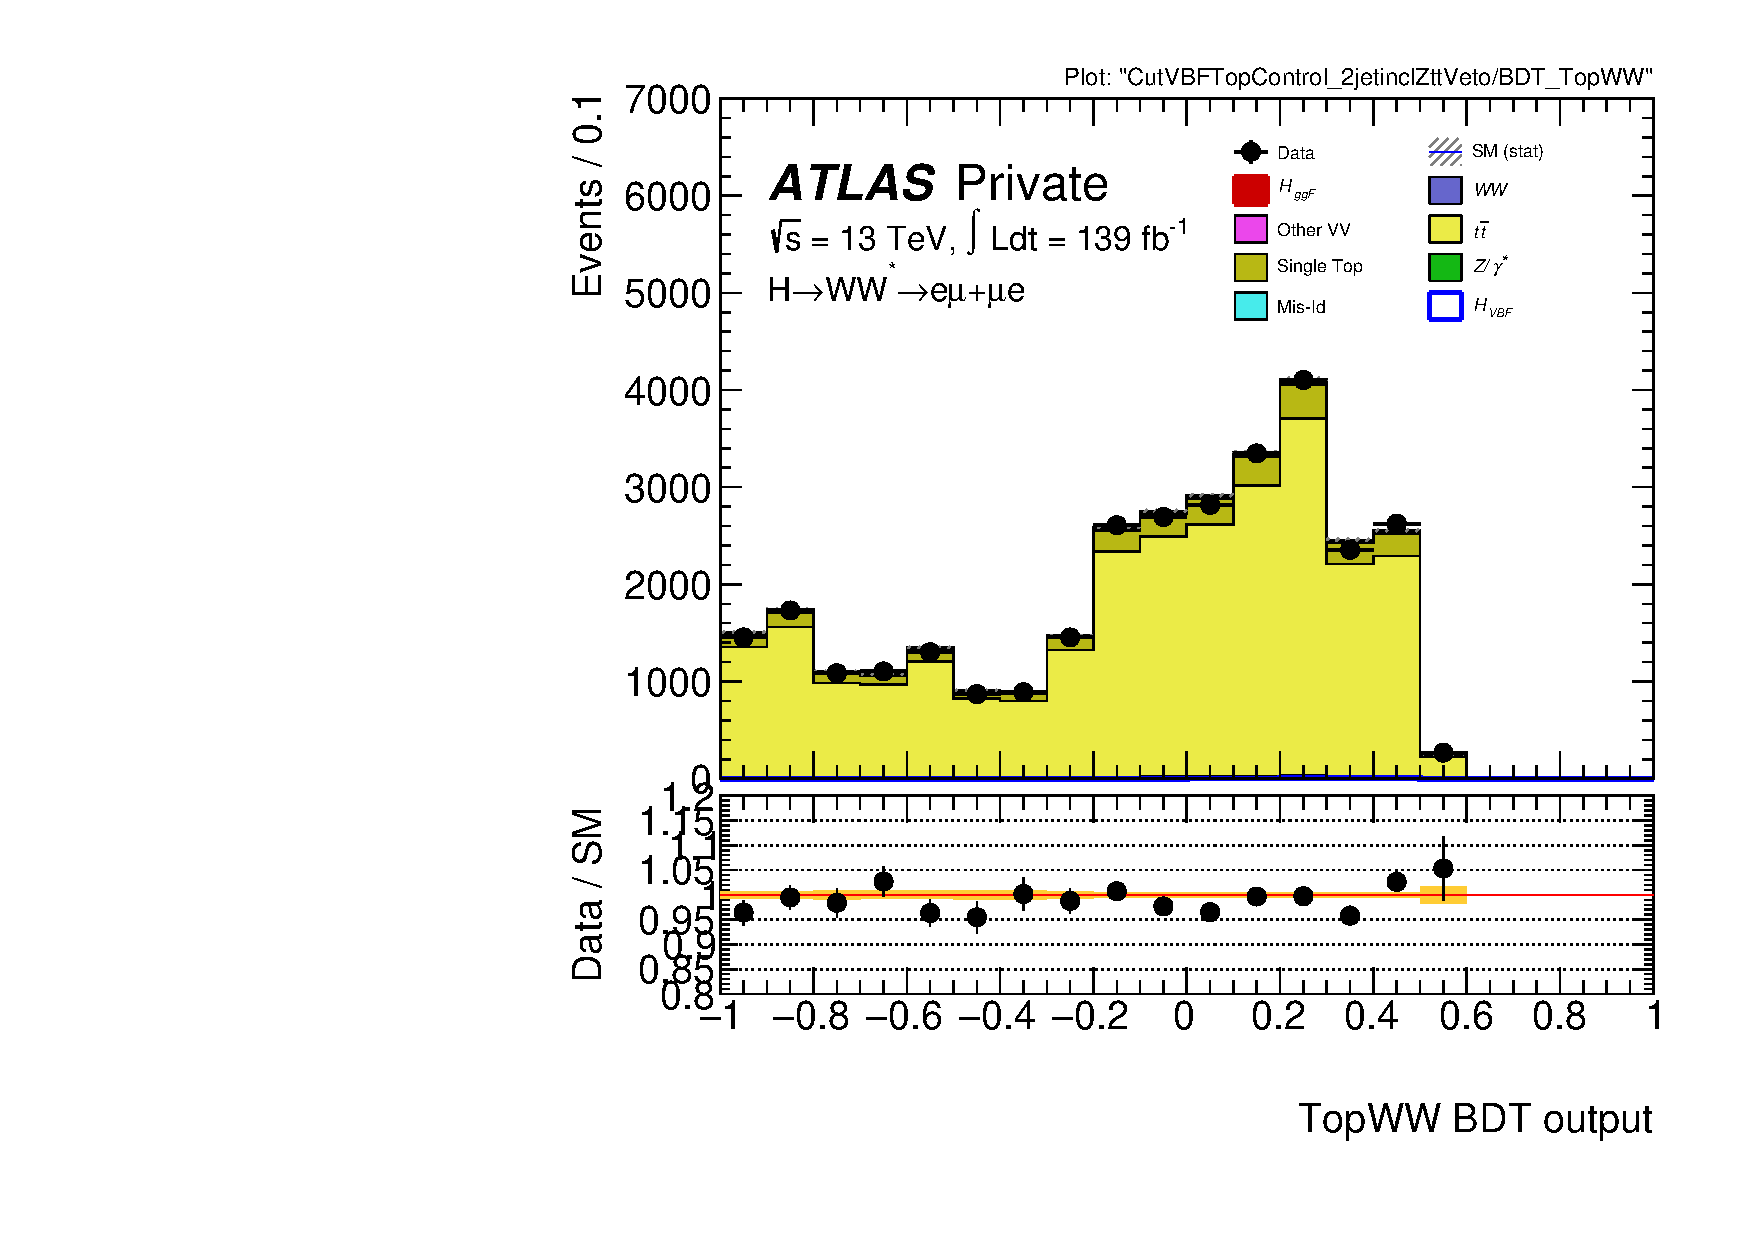
\includegraphics[width=.5\linewidth]{Pictures/run2-emme-CutVBFTopControl_2jetinclZttVeto-BDT_TopWW-lin.pdf}
\caption{Full weighted samples of all signal and background plotted over Top vs. $WW$ BDT output distributions in top validation region}
\label{fig:TopWWBDTVR}
\end{figure}

Normalization factors (NF) are derived in the top validation region to correct for data/MC mis-modelling. These factors are applied to the top sample in the signal region. The NF factors are $0.99\pm0.01$. 

\subsection{Diboson background}

The $WW$ background consists primarily of QCD $WW$+jets events (highly dominating electroweak vertices). This background is estimated along with the top background using a joint parameter due to their similarities in signature as well as the difficulty in defining a pure $WW$ control region without top contamination. A $WW$ validation region is defined to demonstrate $WW$ MC modelling in a targeted $WW$ region.  The $WW$ validation region is defined with at least 2 jets, a $b$-veto ($N_{b-jet}<1$) and a central-jet-veto of below $20$GeV as in the signal region. Two additional cuts differ from the signal region: $m_T>130$GeV and $m_{T2}>160$GeV where $m_{T2}$ is defined as
\begin{equation}
m_{T2}=min_{p_T^1+p_T^2=p_T}(max(m_T^2(p_T^1,p_T^a),m_T^2(p_T^2,p_T^b)))
\end{equation}
This represents a lower bound on the parent particle's mass, so using a large $m_{T2}$ cut eliminates contamination from many $t\bar{t}$ decays which have an upper limit near the top mass. The purity of the region is $\approx 37\%$ and the cutflow for this region is shown below.

\begin{table}[h!]
\scalebox{0.35}{
%%% created on Thu Jun 11 11:37:17 2020 from TQSampleFolder 'samples' with TQLibrary UNKNOWN compiled with GCC 8.3.0 against ROOT 6.16/00
\providecommand{\xmark}{{\sffamily \bfseries X}}
\providecommand\rotatecell[2]{\rotatebox[origin=c]{#1}{#2}}
\begin{tabular}{ r ||r  r  r | r | r  r  r | r   r }
\ensuremath{\mathcal{L}=139 fb^{-1}} & $H_{VBF}$ & $H_{ggF}$ & $H_{VH}/ttH$ & Diboson & Top & Zjets & Mis-Id & Data & Data/MC\tabularnewline
\hline
b-veto & \ensuremath{323.67\pm 0.54} & \ensuremath{1109.94\pm 3.42} & \ensuremath{437.85\pm 1.22} & \ensuremath{25106.71\pm 97.05} & \ensuremath{63787.91\pm 57.22} & \ensuremath{22151.24\pm 102.73} & \ensuremath{3793.55\pm 70.69} & \ensuremath{109677} & \ensuremath{0.94\pm 0.00}\tabularnewline
$M_{T}>$130 GeV & \ensuremath{32.37\pm 0.17} & \ensuremath{155.17\pm 1.28} & \ensuremath{59.98\pm 0.44} & \ensuremath{18021.15\pm 51.26} & \ensuremath{50088.35\pm 50.83} & \ensuremath{872.43\pm 33.66} & \ensuremath{1784.17\pm 49.41}  & \ensuremath{68255} & \ensuremath{0.96\pm 0.00}\tabularnewline
$M_{T2}>$160 GeV & \ensuremath{18.87\pm 0.13} & \ensuremath{62.44\pm 0.82} & \ensuremath{17.29\pm 0.24} & \ensuremath{7271.80\pm 35.96} & \ensuremath{11553.13\pm 24.82} & \ensuremath{302.42\pm 14.17} & \ensuremath{515.71\pm 26.44} & \ensuremath{18672} & \ensuremath{0.95\pm 0.01}\tabularnewline
CJV (20GeV) & \ensuremath{13.61\pm 0.11} & \ensuremath{40.50\pm 0.66} & \ensuremath{11.30\pm 0.20} & \ensuremath{4861.01\pm 32.55} & \ensuremath{6415.93\pm 19.00} & \ensuremath{184.81\pm 12.88} & \ensuremath{327.54\pm 20.73}  & \ensuremath{11245} & \ensuremath{0.95\pm 0.01}\tabularnewline
\hline
\end{tabular}

}
\caption{Cutflow in the $WW$ validation region.}
\label{tab:wwvr}
\end{table}

Data/MC shows good agreement over various variable distributions as seen below. 
\begin{figure}[!h]
\centering
%  \subfloat[$m_{\ell\ell}$]{
%      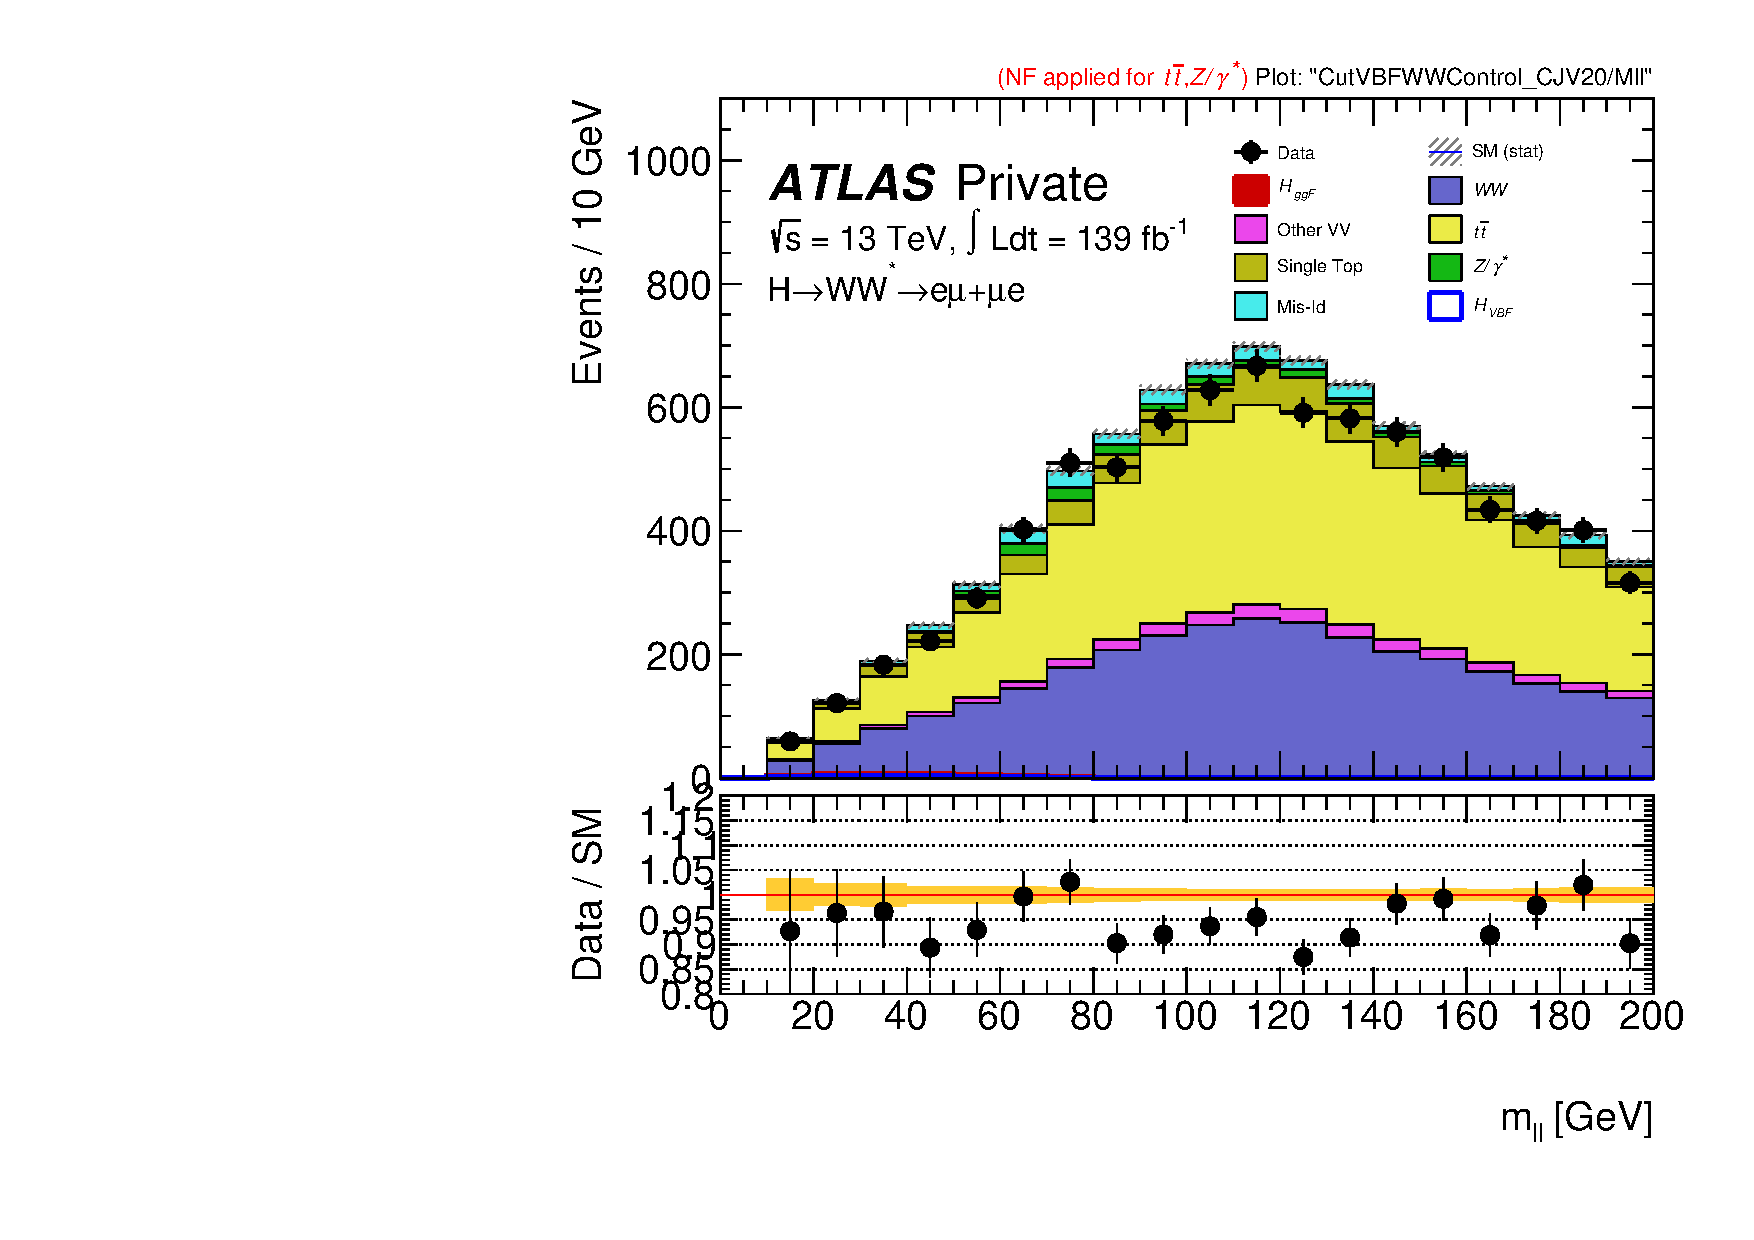
\includegraphics[width=0.3\textwidth]{Pictures/run2-emme-CutVBFWWControl_CJV20-Mll-lin.pdf}
%  }\hfill
  \subfloat[$\Delta Y_{\ell\ell}$]{
      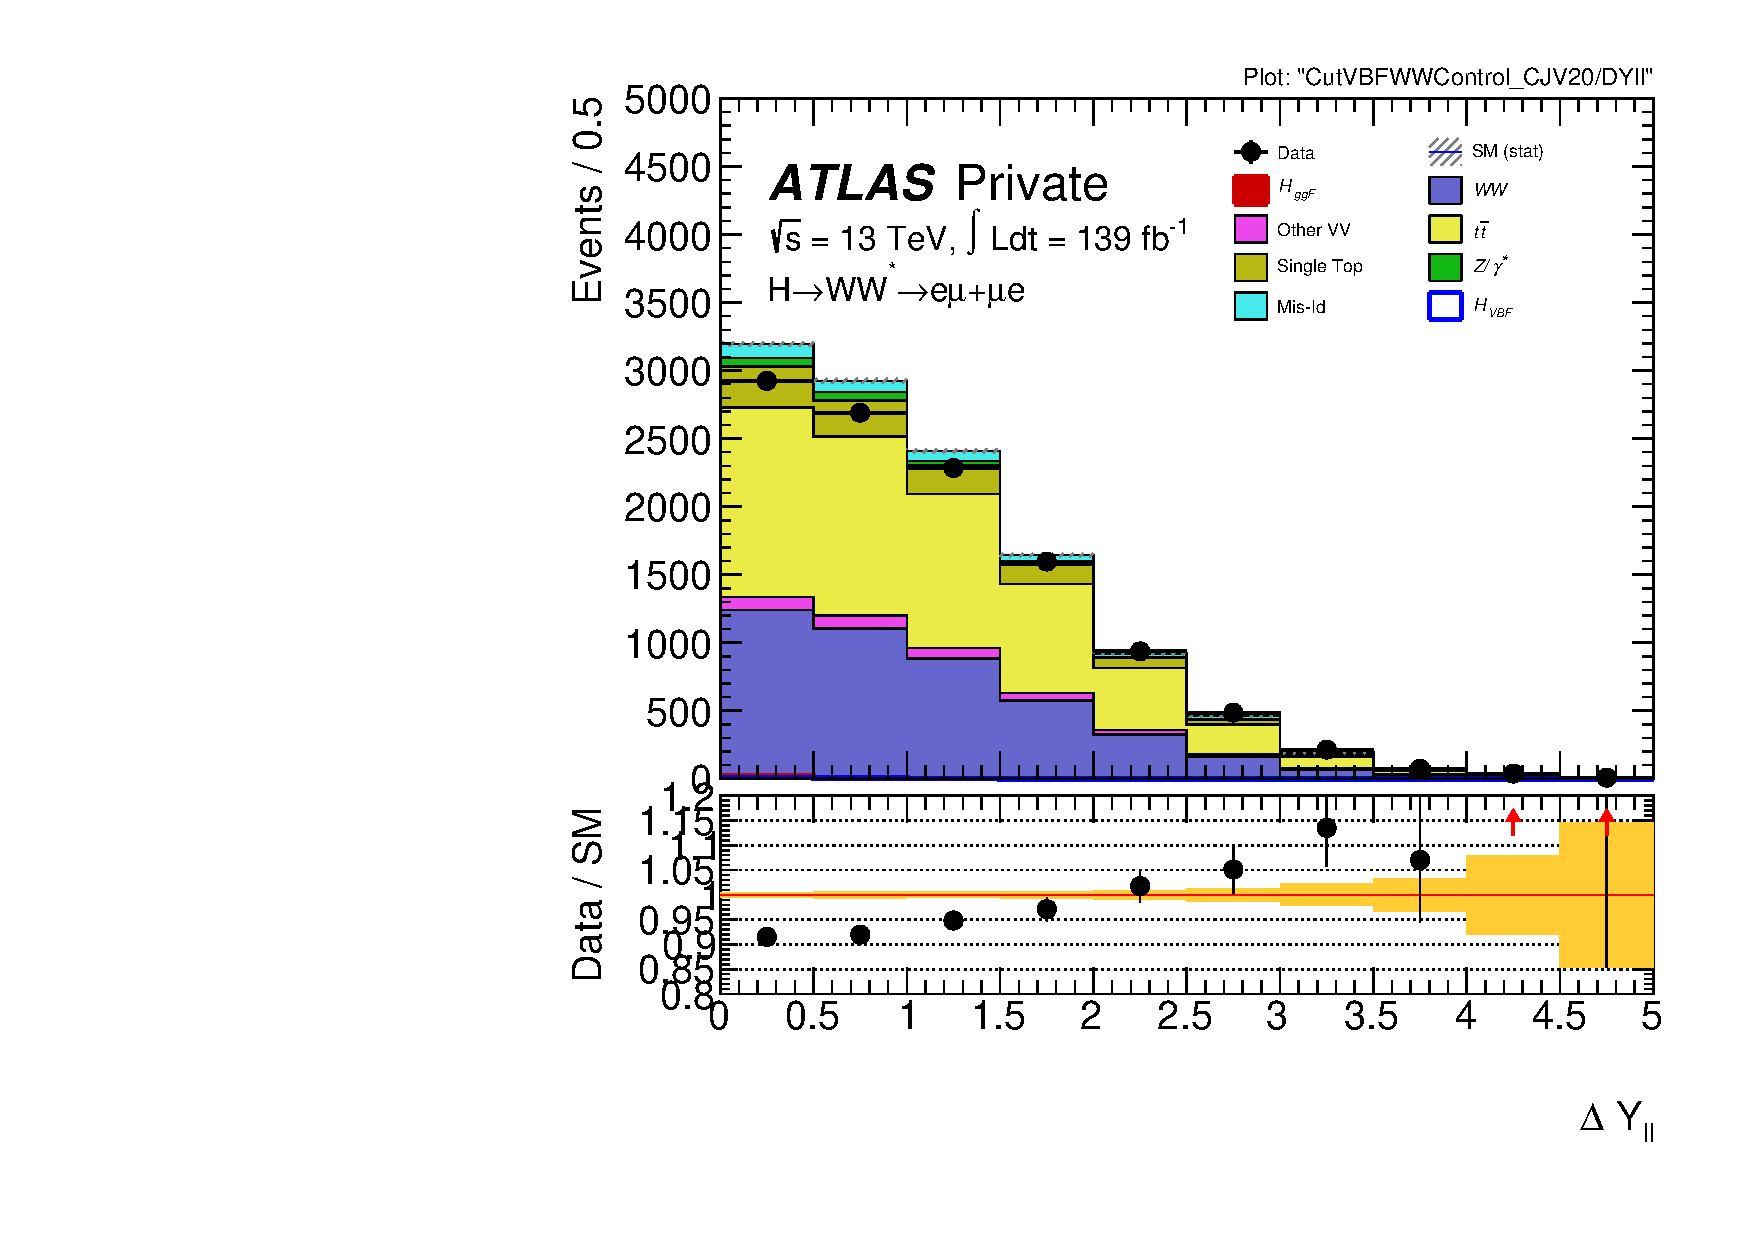
\includegraphics[width=0.3\textwidth]{Pictures/run2-emme-CutVBFWWControl_CJV20-DYll-lin.pdf}
  }\hfill
  \subfloat[$\Delta Y_{jj}$]{
      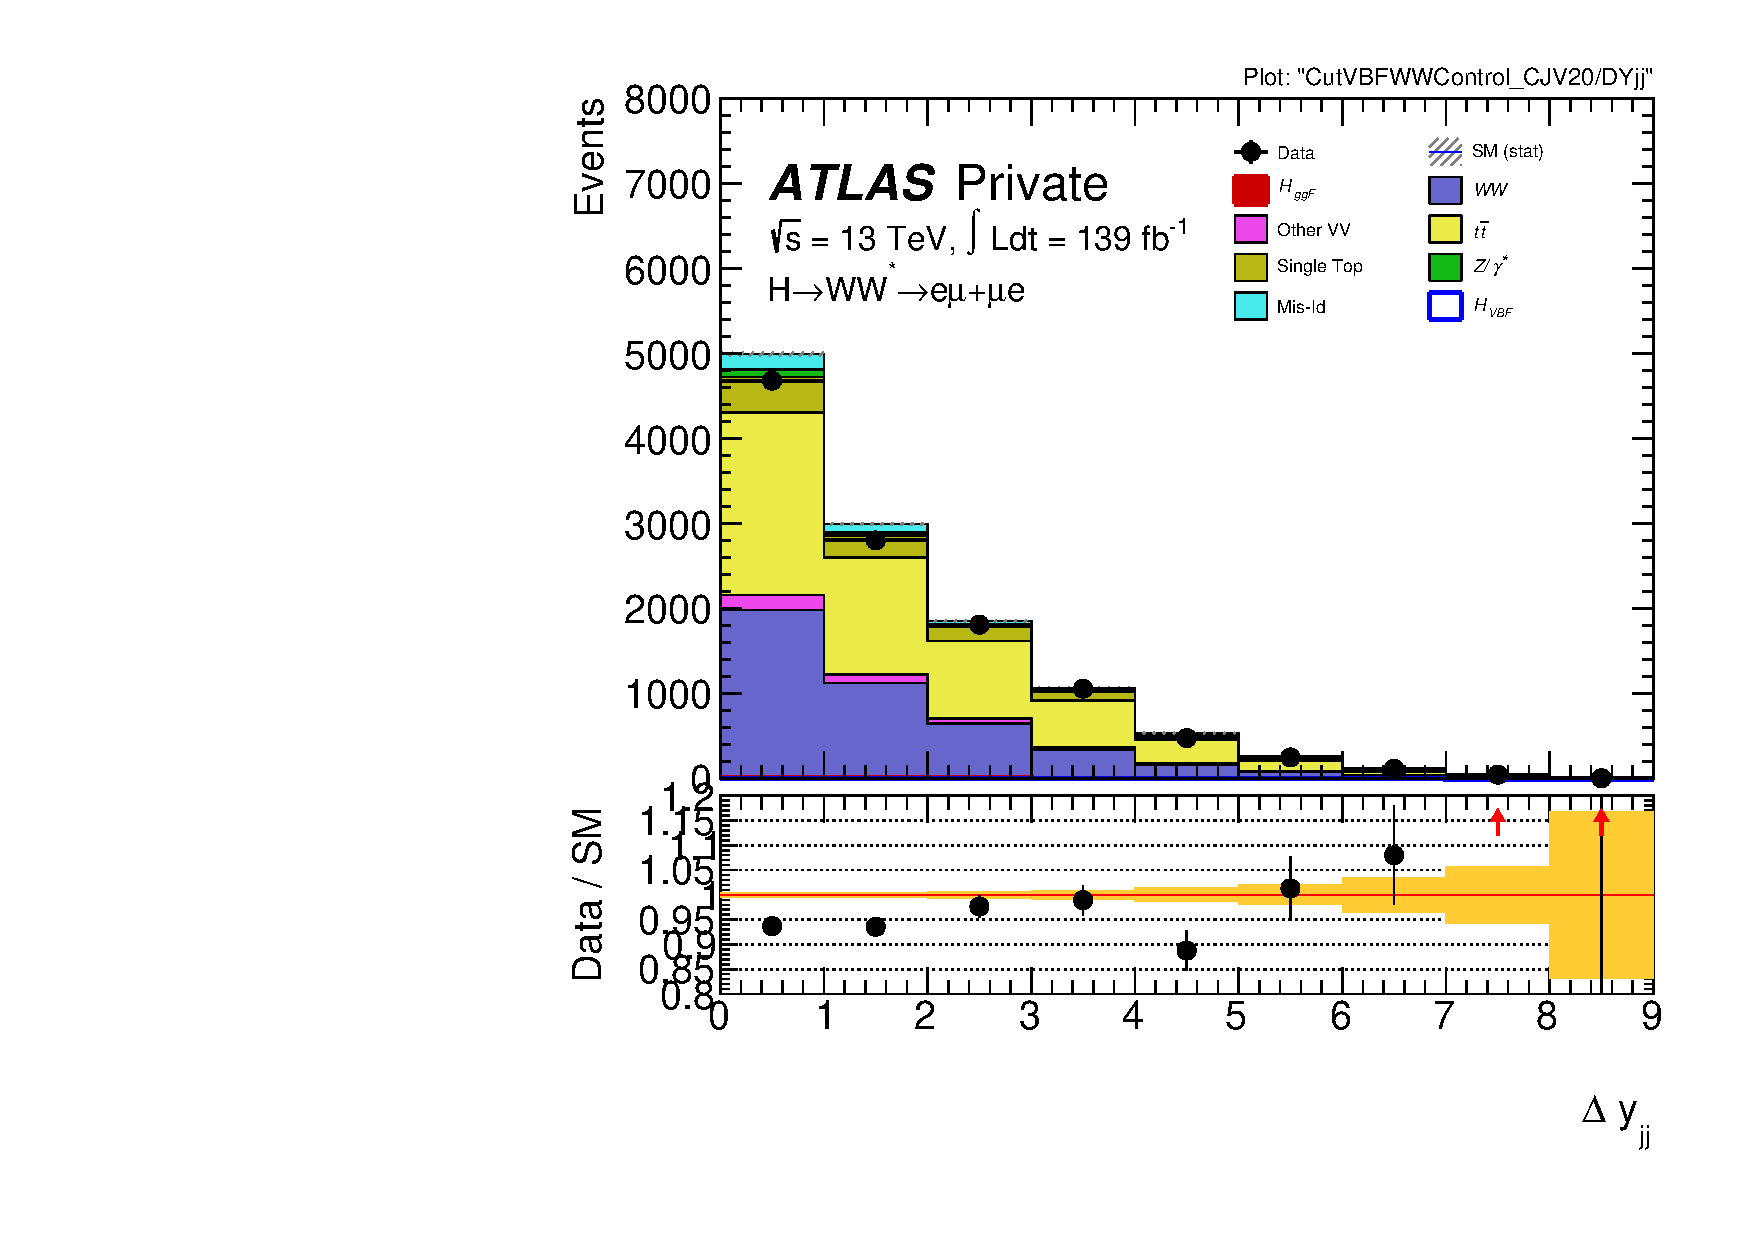
\includegraphics[width=0.3\textwidth]{Pictures/run2-emme-CutVBFWWControl_CJV20-DYjj-lin.pdf}
  }\hfill
  \subfloat[$\sum$ centralities]{
      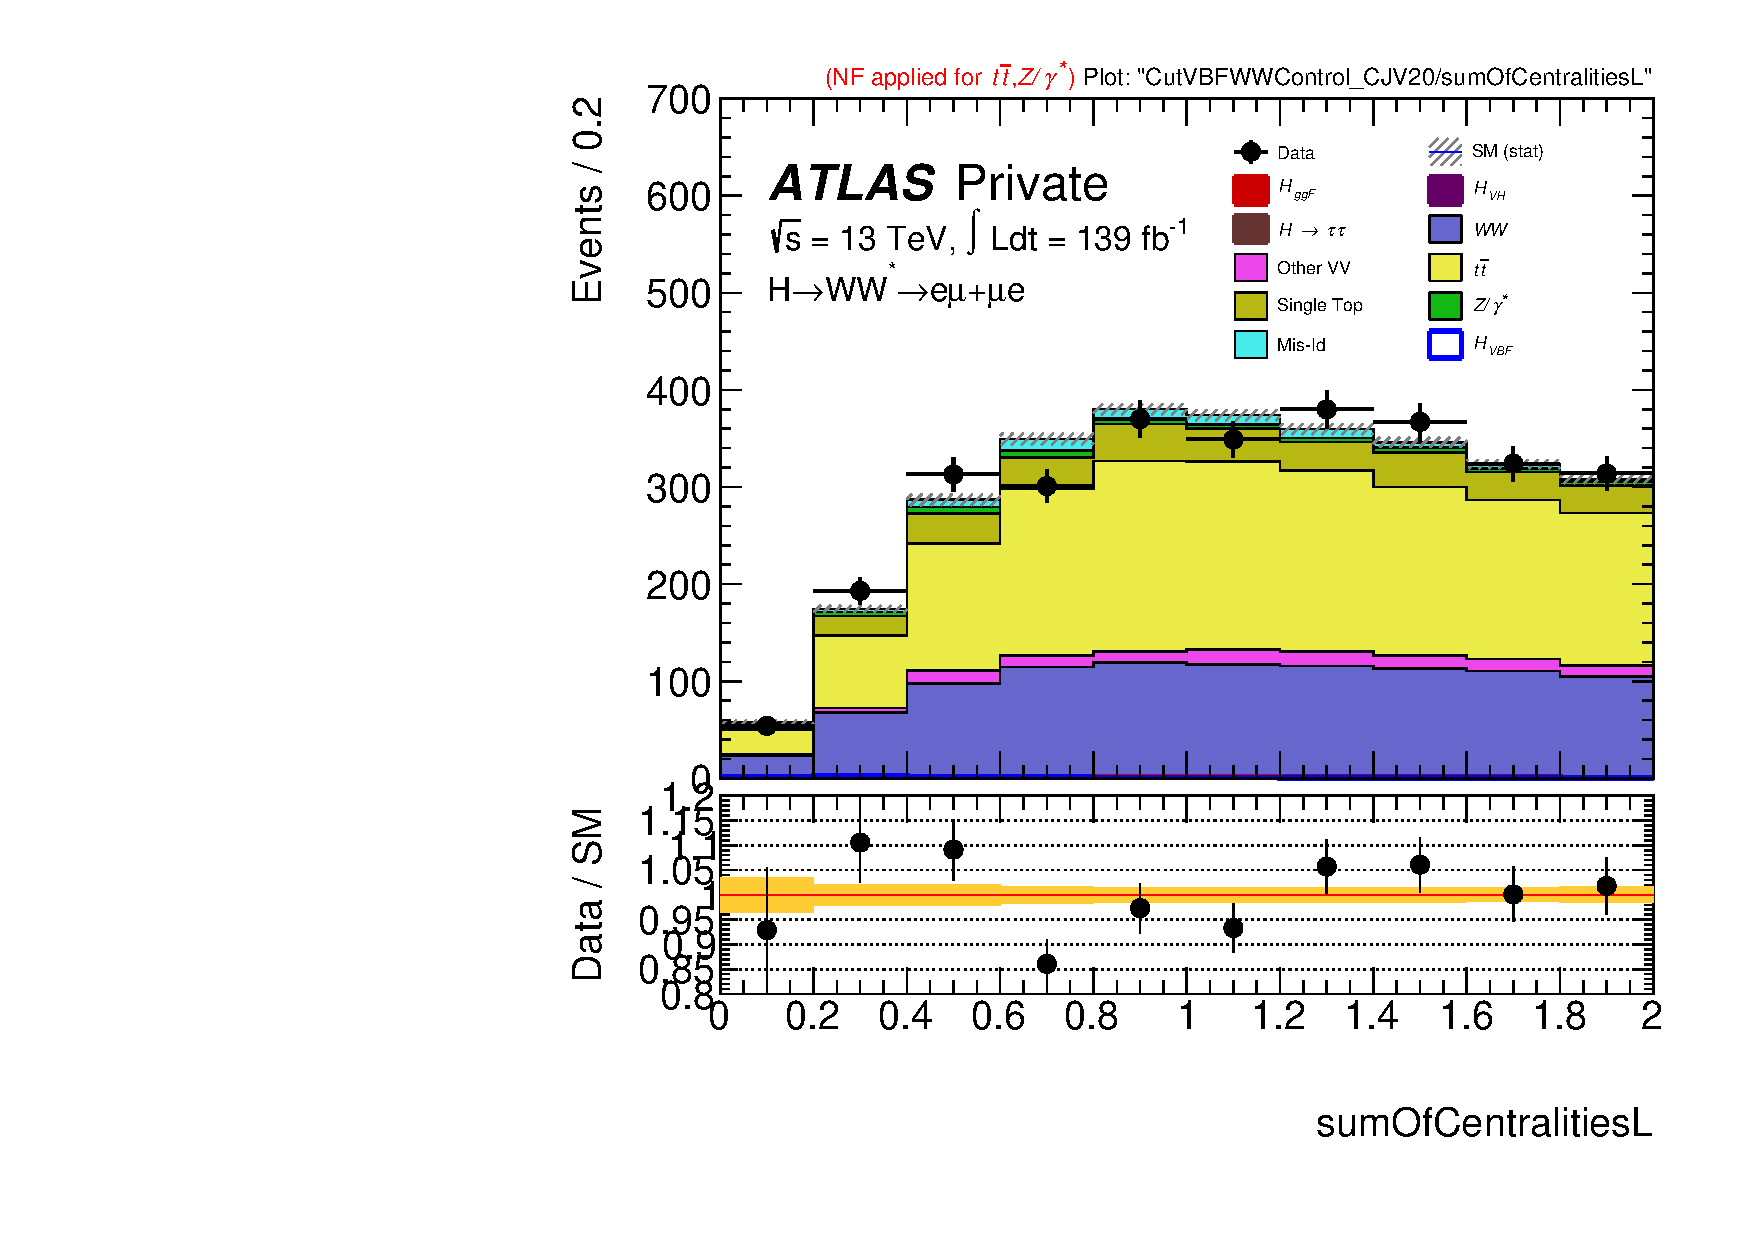
\includegraphics[width=0.3\textwidth]{Pictures/run2-emme-CutVBFWWControl_CJV20-sumOfCentralitiesL-lin.pdf}
  }\hfill
  \subfloat[$M_{l0j0}$]{
      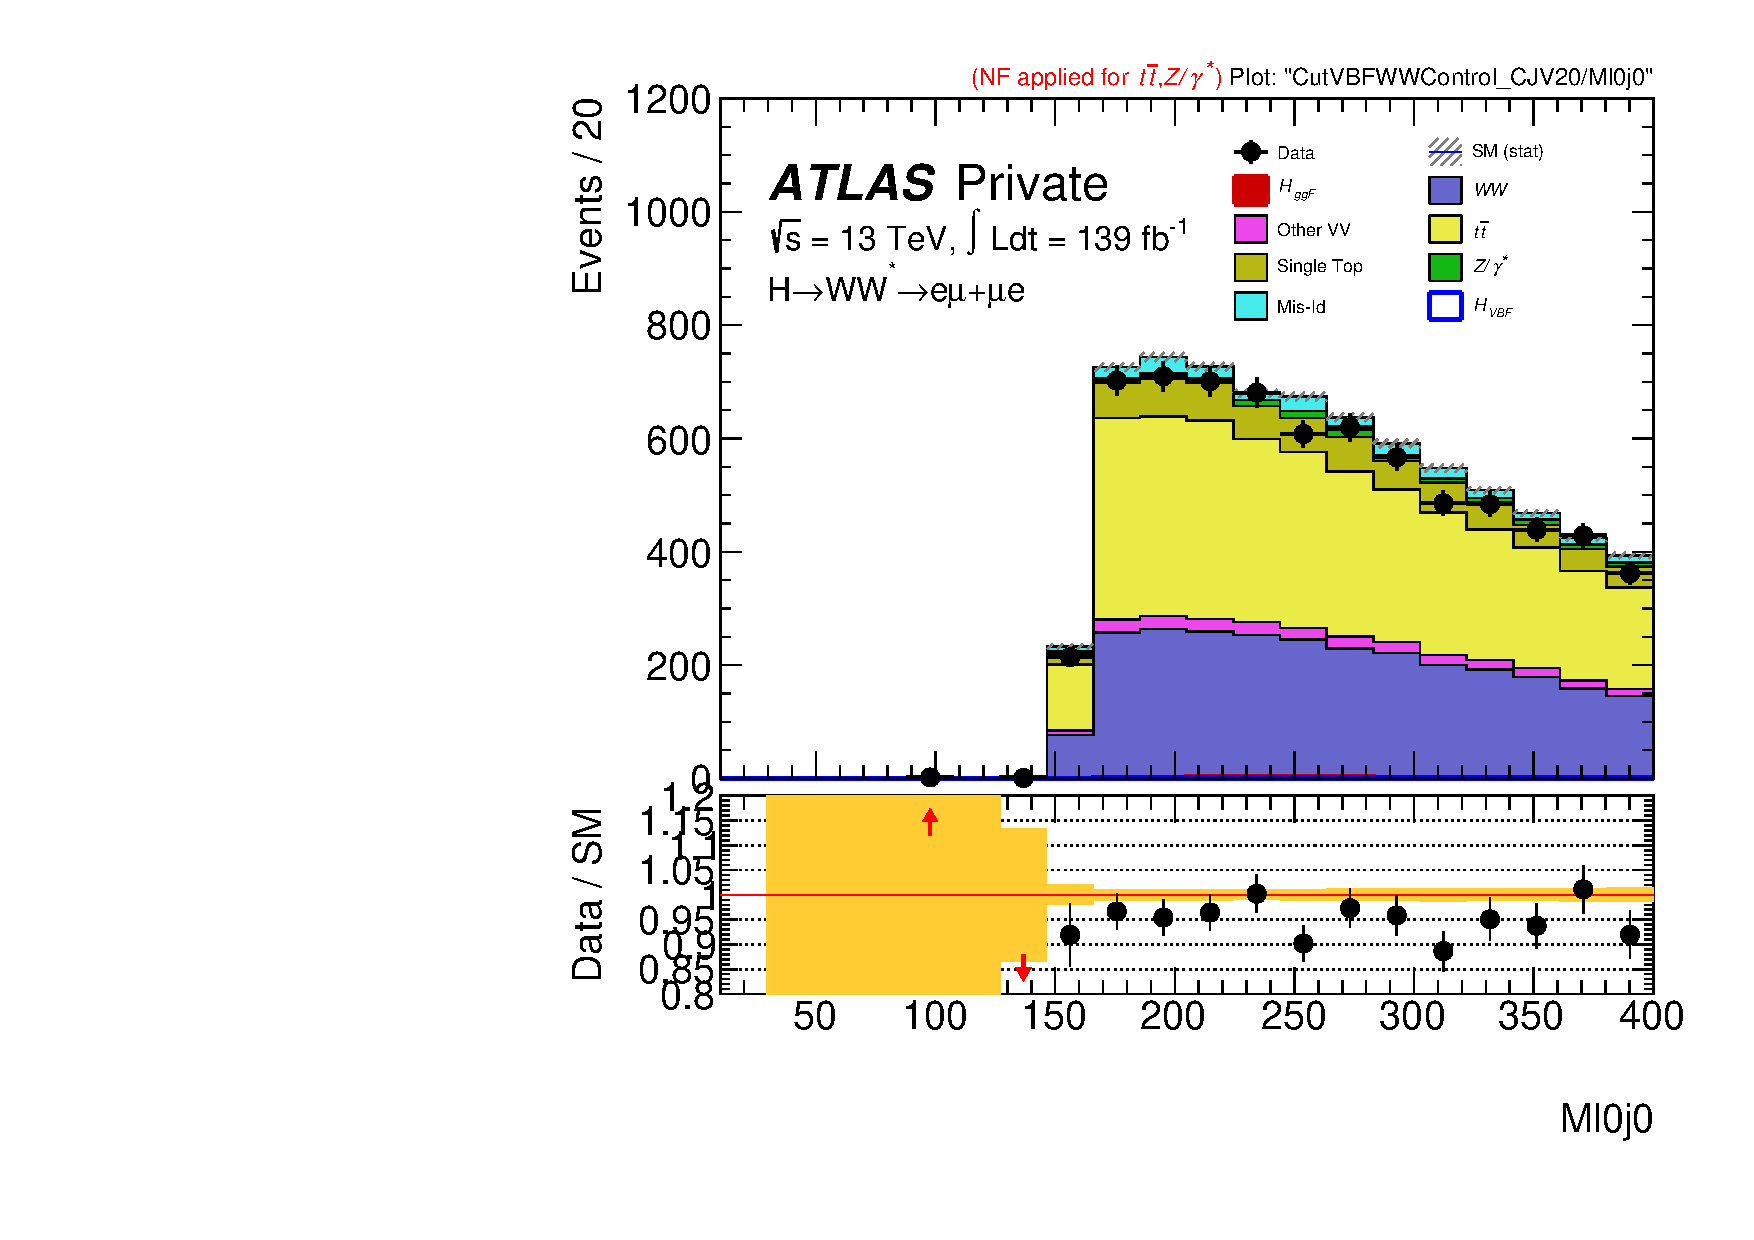
\includegraphics[width=0.3\textwidth]{Pictures/run2-emme-CutVBFWWControl_CJV20-Ml0j0-lin.pdf}
  }\hfill
  \subfloat[$M_{l1j1}$]{
      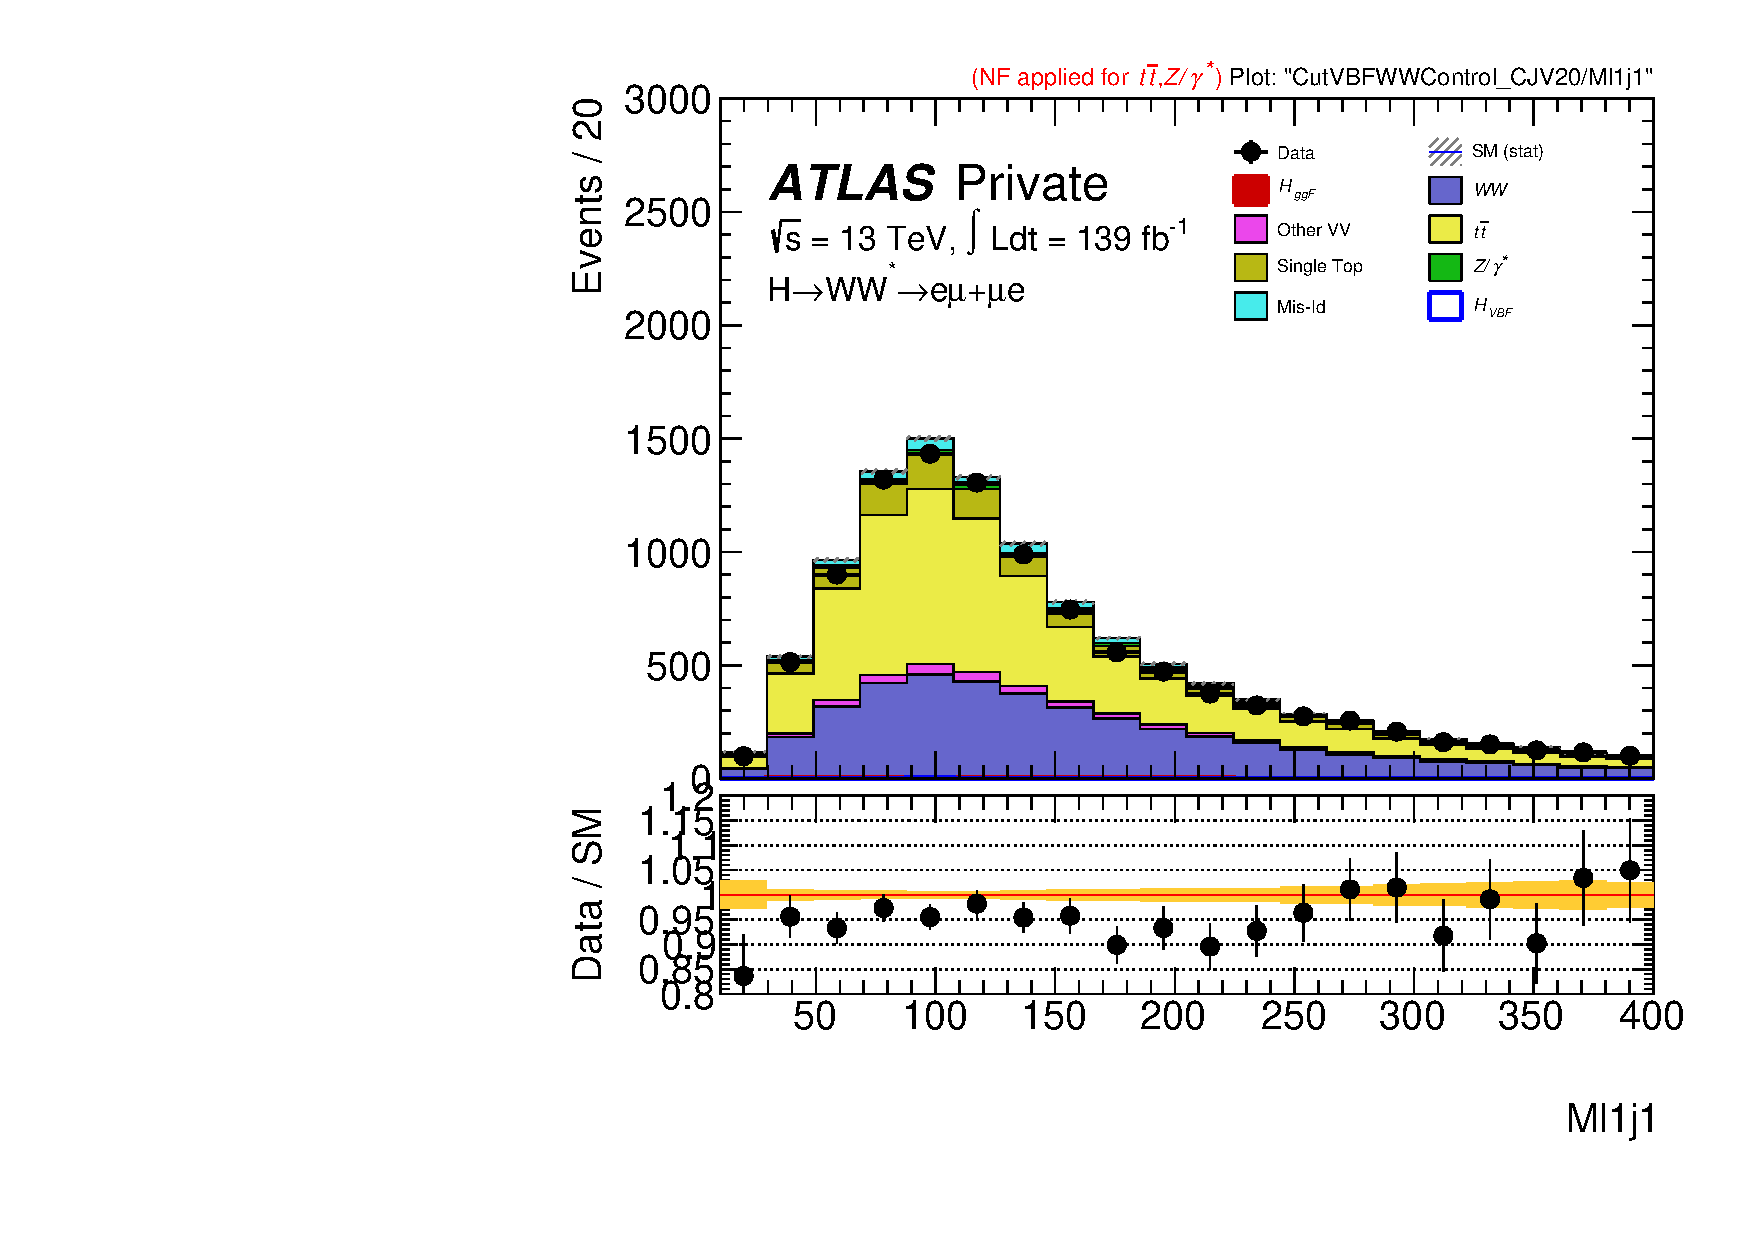
\includegraphics[width=0.3\textwidth]{Pictures/run2-emme-CutVBFWWControl_CJV20-Ml1j1-lin.pdf}
  }\hfill
  \subfloat[$p_T^{j0}$]{
      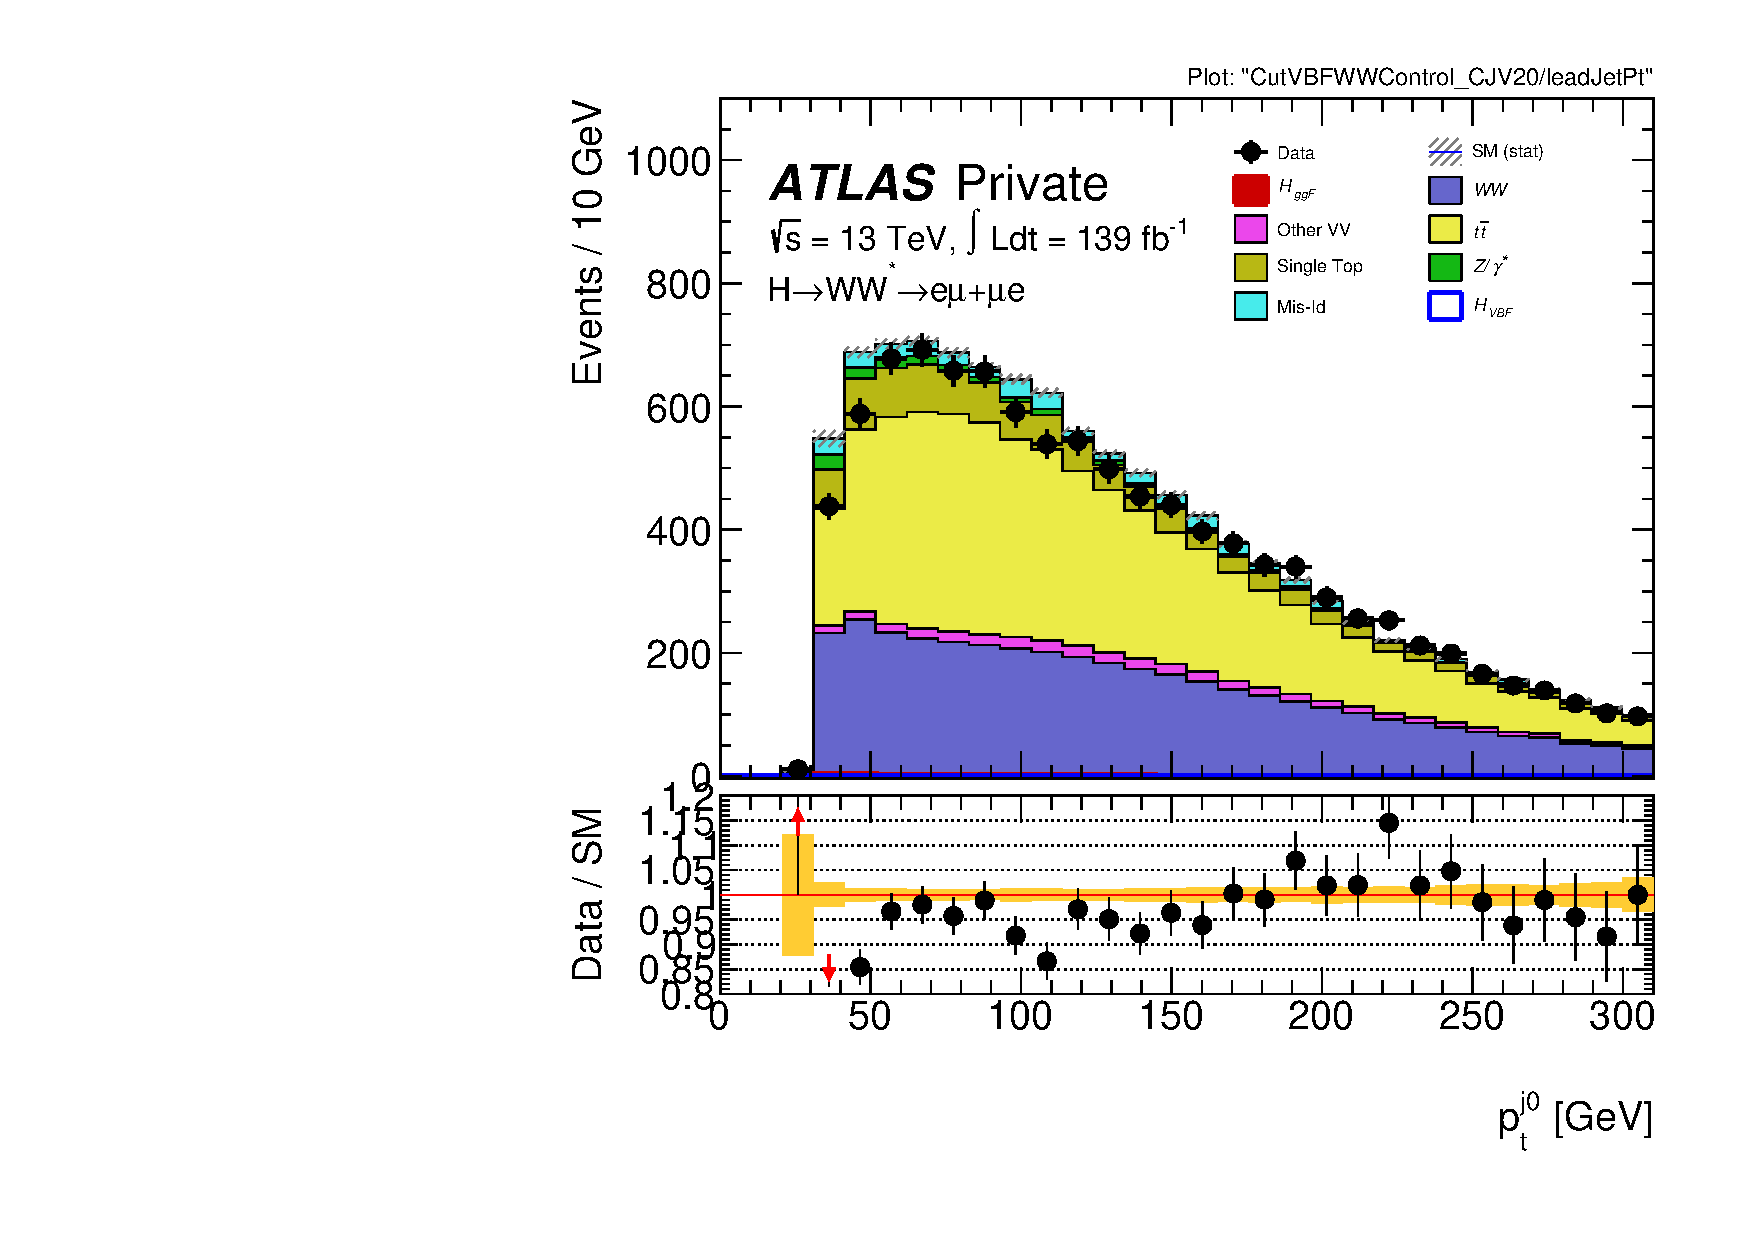
\includegraphics[width=0.3\textwidth]{Pictures/run2-emme-CutVBFWWControl_CJV20-leadJetPt-lin.pdf}
  }\hfill
%  \subfloat[$m_{jj}$]{
%      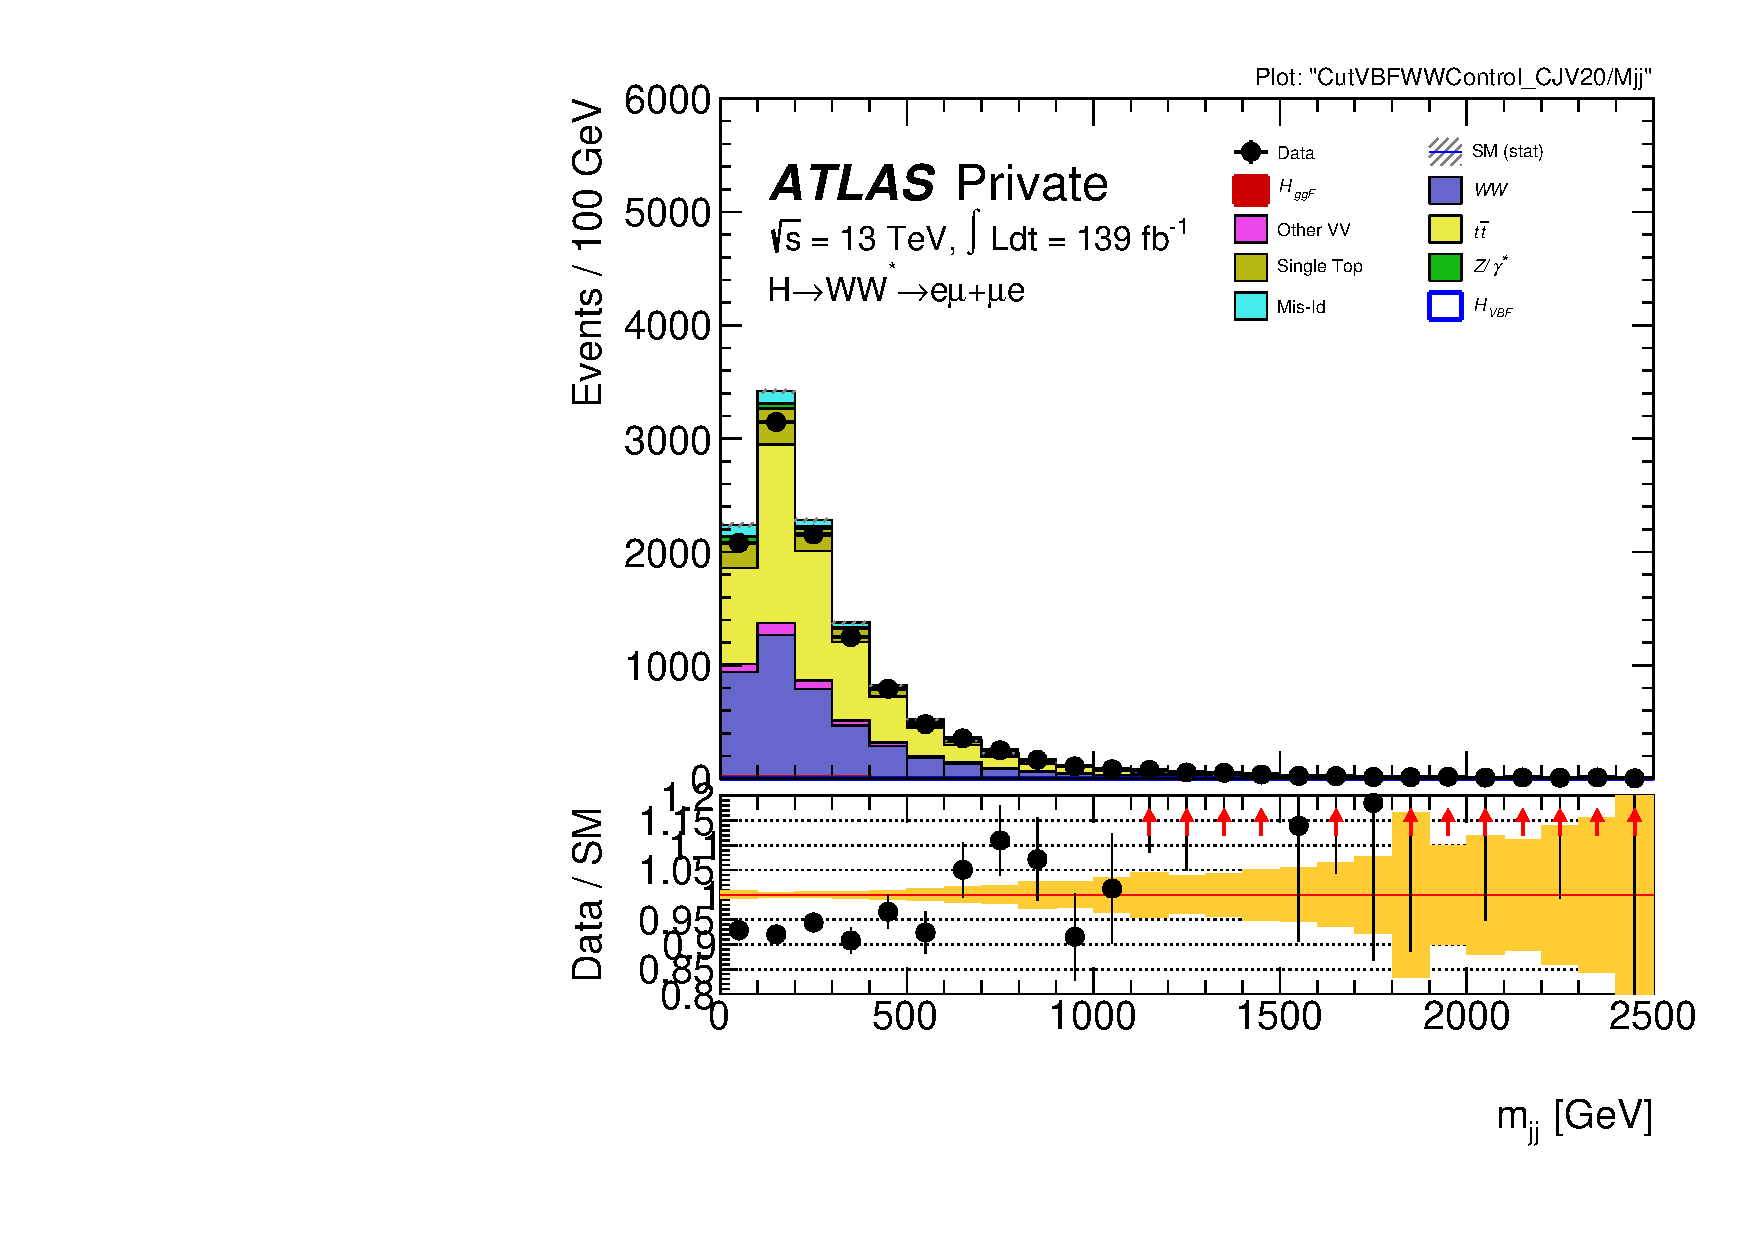
\includegraphics[width=0.3\textwidth]{Pictures/run2-emme-CutVBFWWControl_CJV20-Mjj-lin.pdf}
%  }\hfill
  \subfloat[$\Delta\Phi_{jj}$]{
      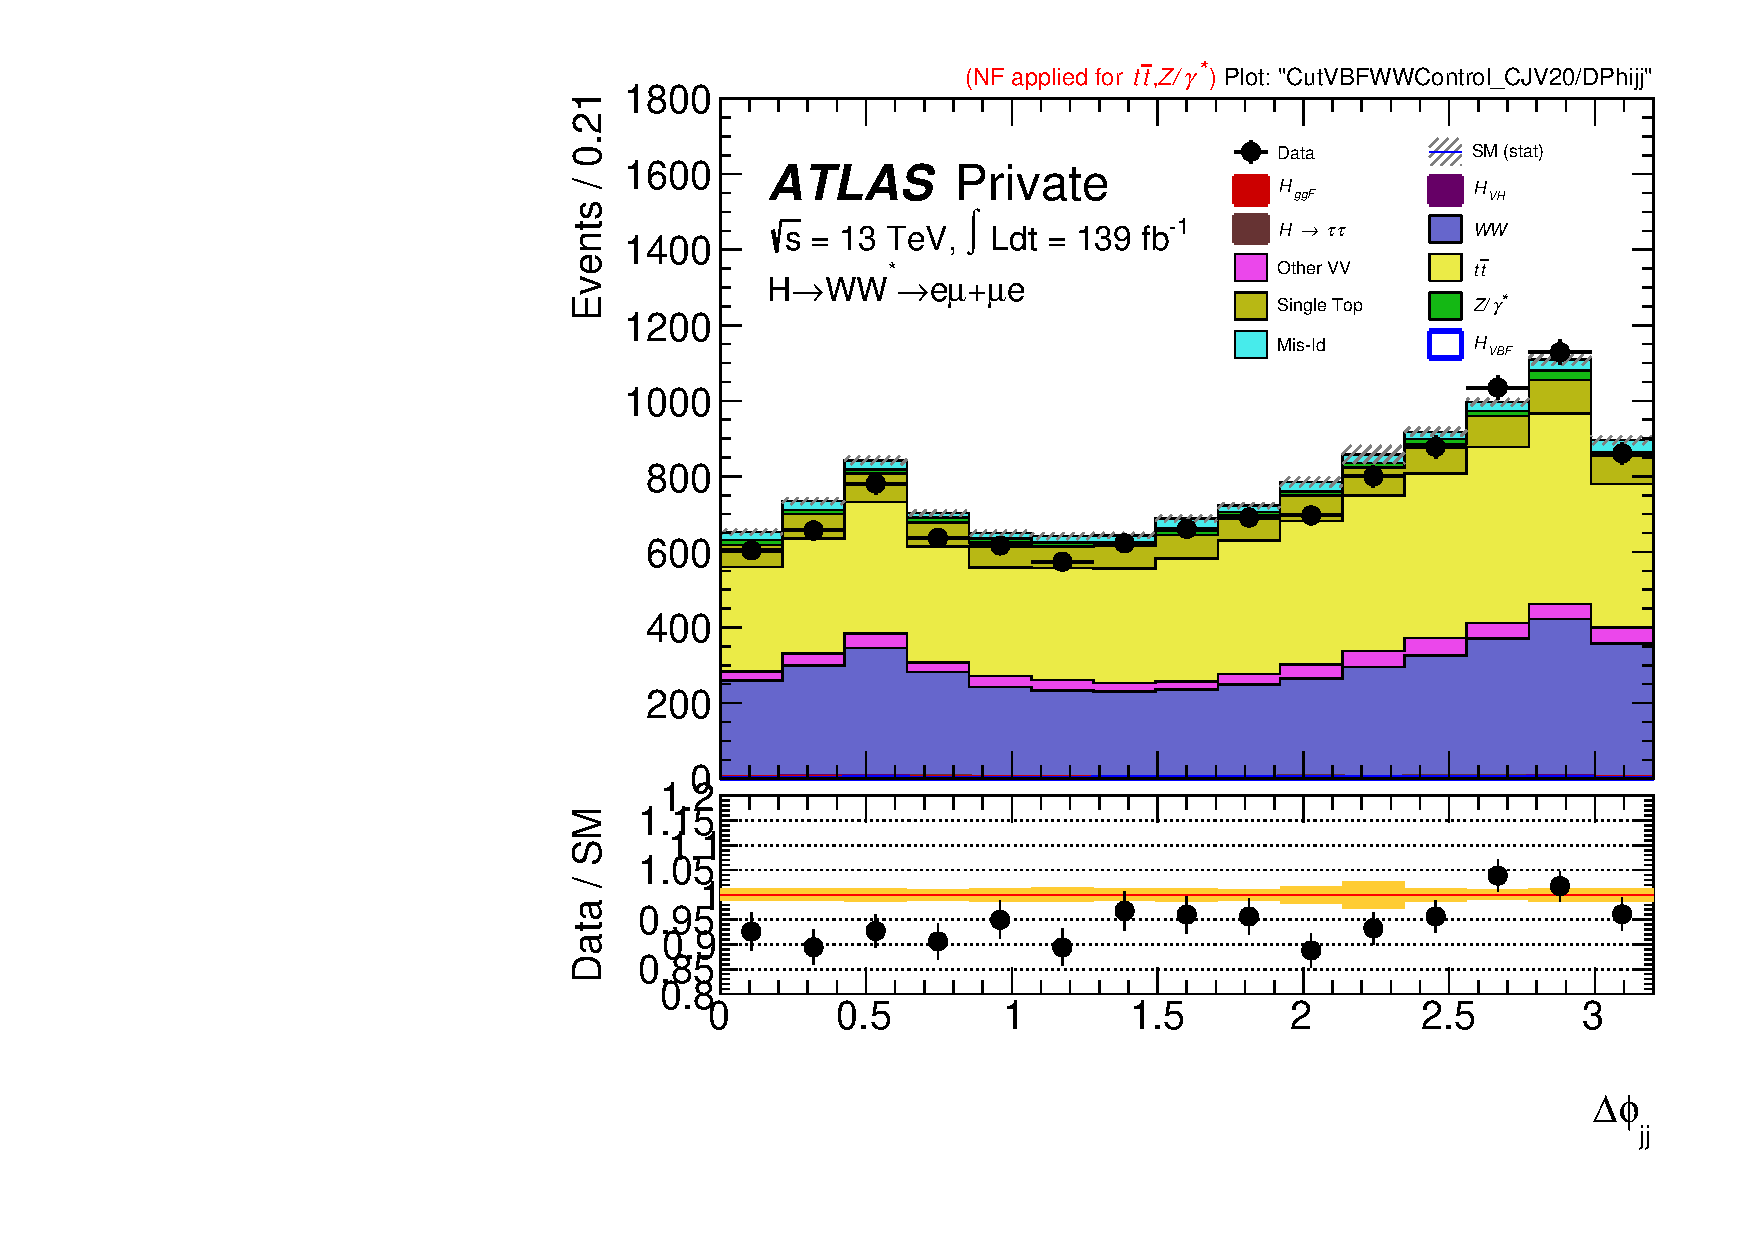
\includegraphics[width=0.3\textwidth]{Pictures/run2-emme-CutVBFWWControl_CJV20-DPhijj-lin.pdf}
  }\hfill
  \subfloat[$p^T_{tot}$]{
      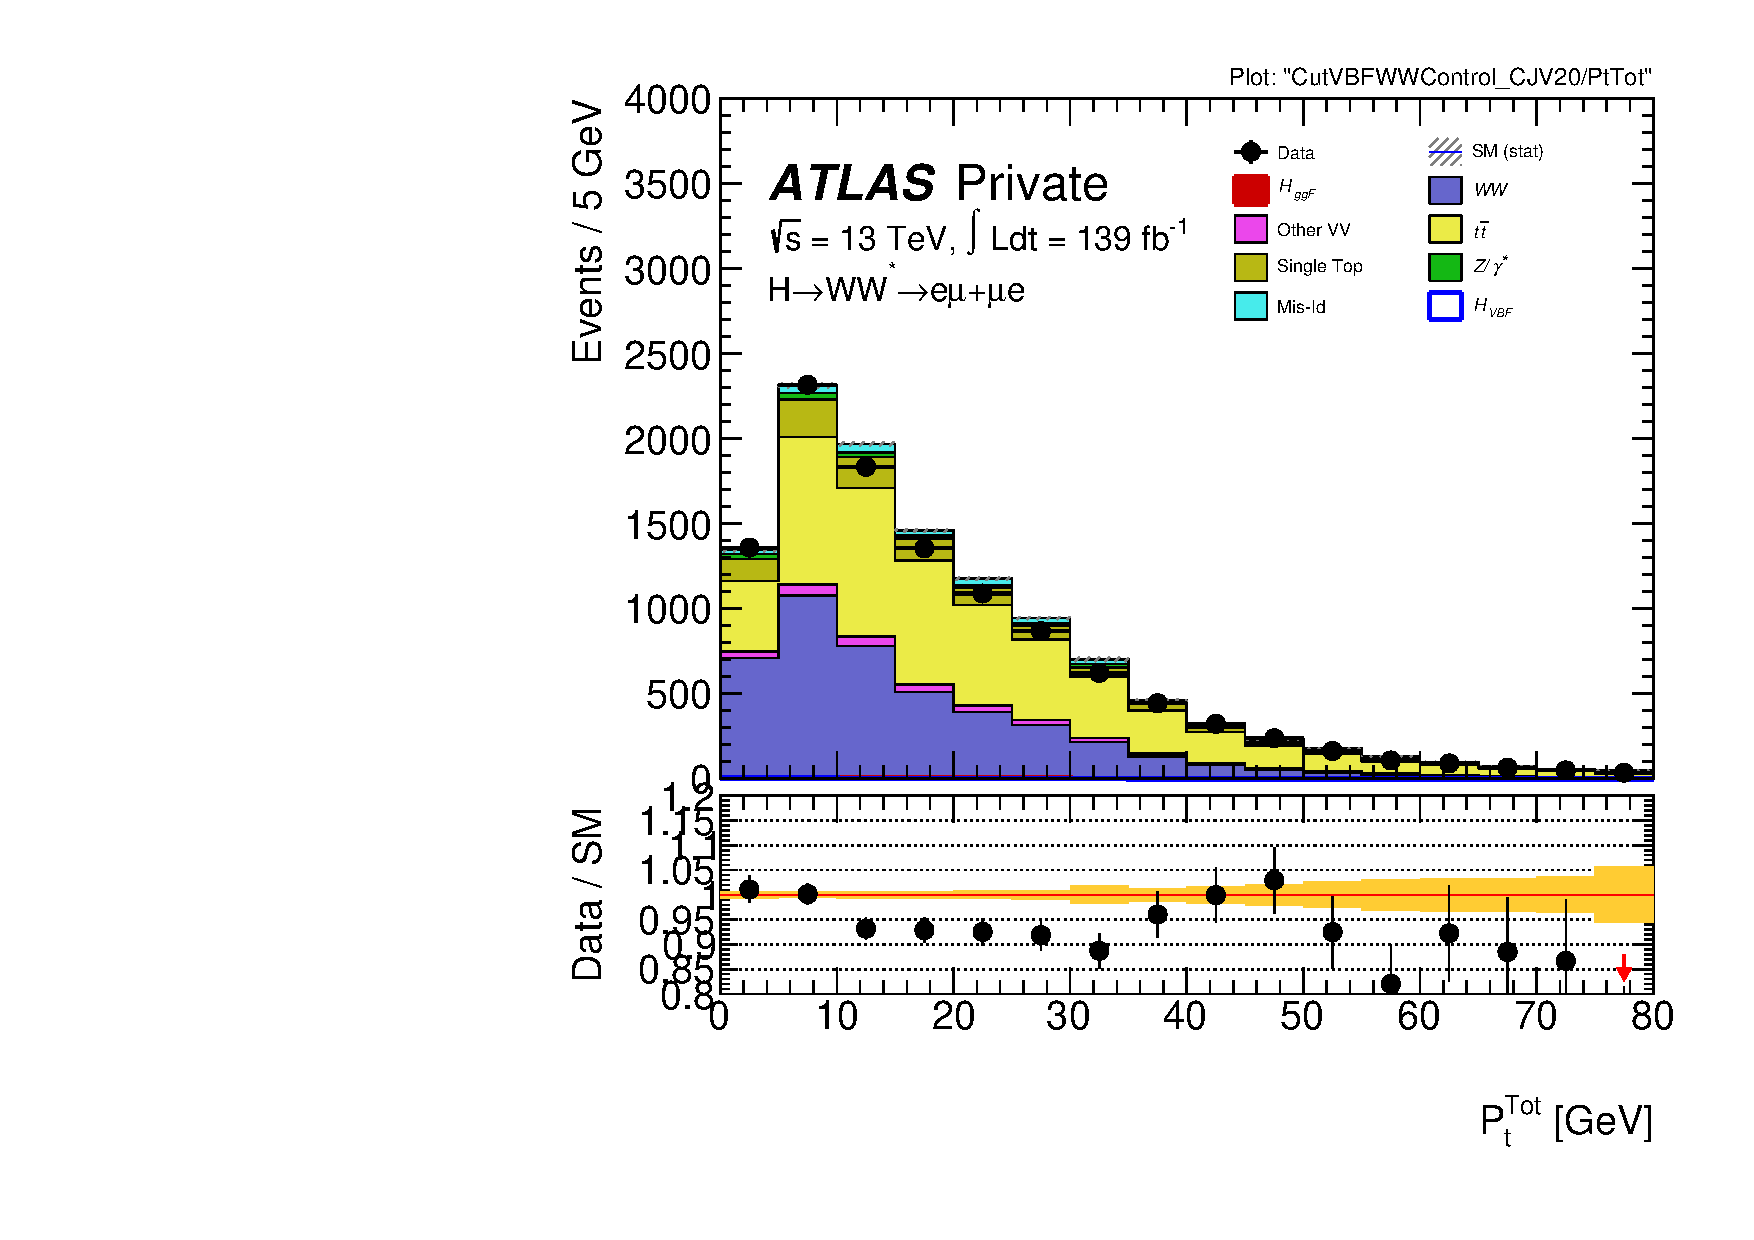
\includegraphics[width=0.3\textwidth]{Pictures/run2-emme-CutVBFWWControl_CJV20-PtTot-lin.pdf}
  }\hfill
  \subfloat[$m_T$]{
      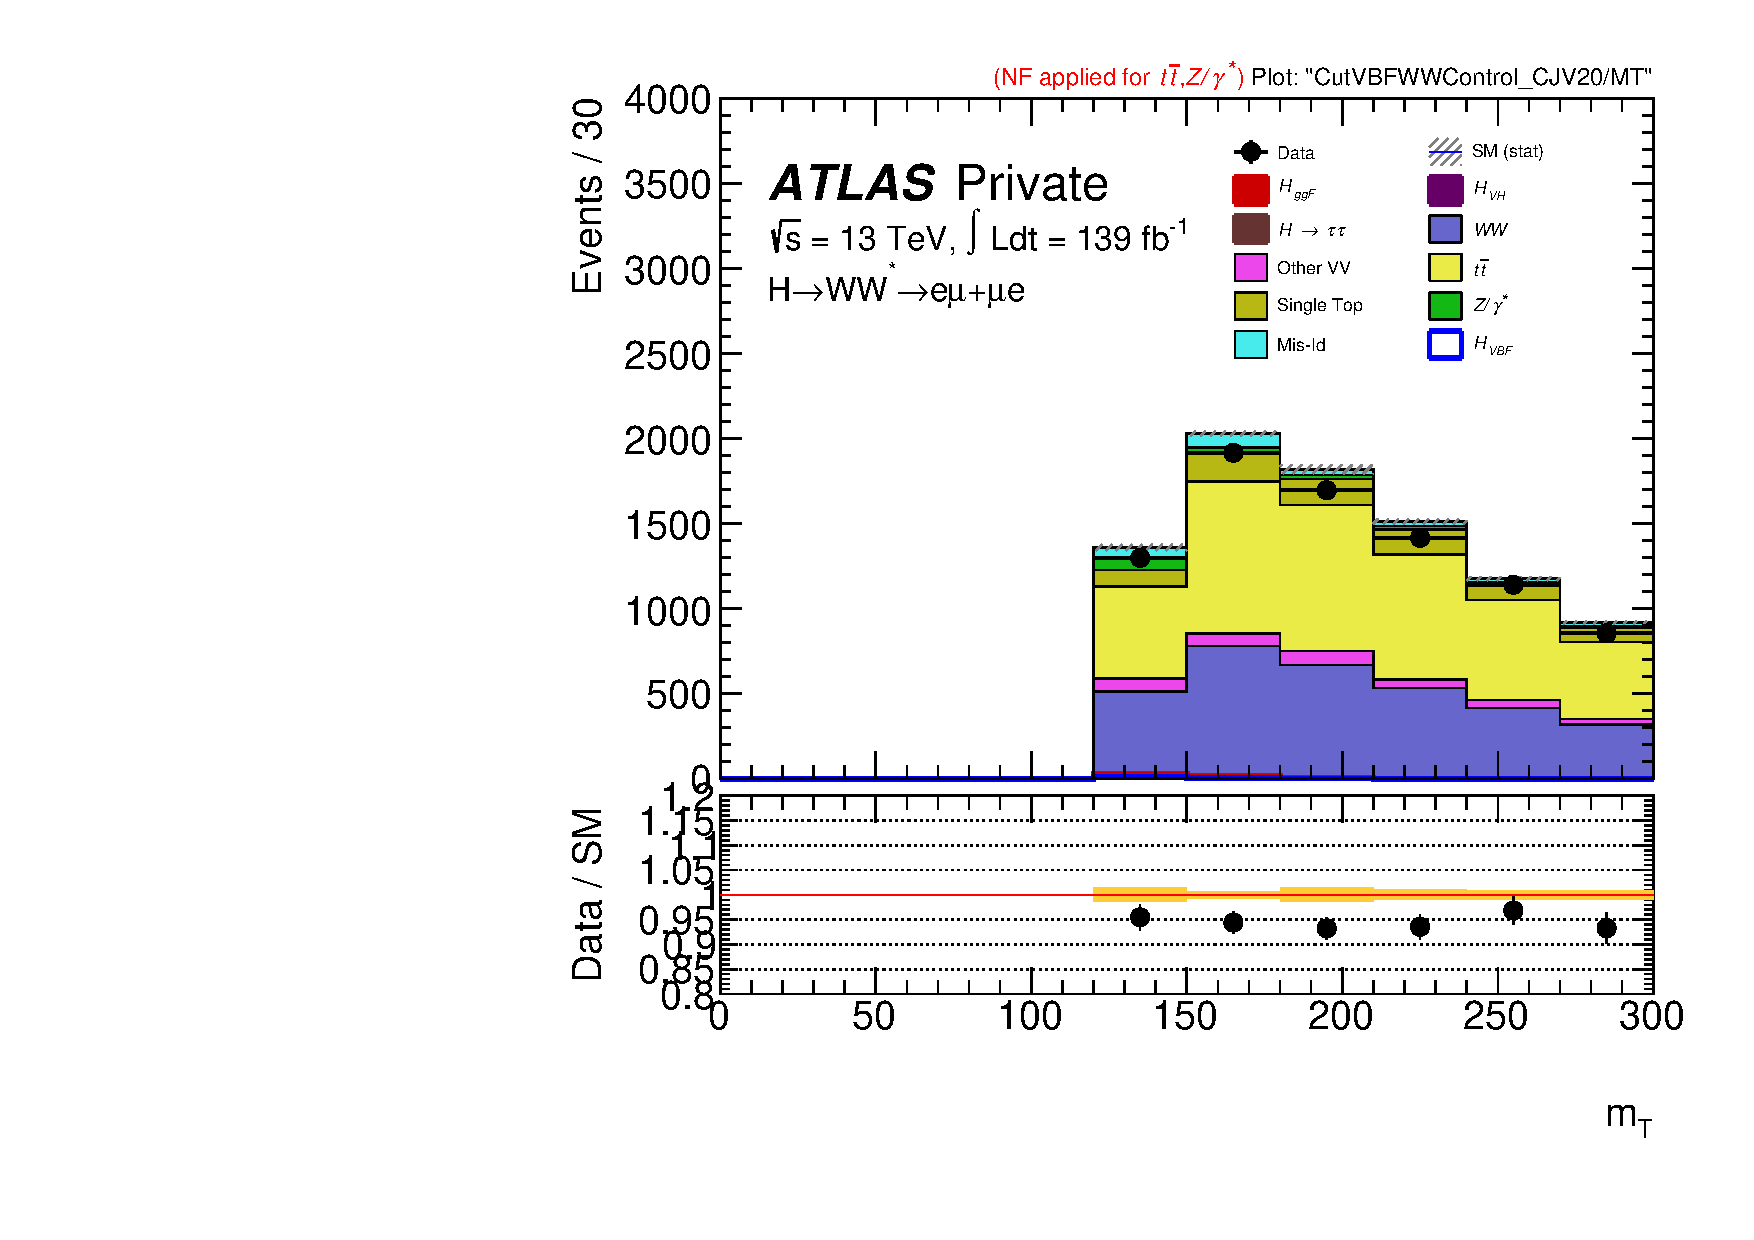
\includegraphics[width=0.3\textwidth]{Pictures/run2-emme-CutVBFWWControl_CJV20-MT-lin.pdf}
  }%\hfill
%  \subfloat[$\ensuremath{E_{\text{T,rel}}^{\text{miss}}}$]{
%      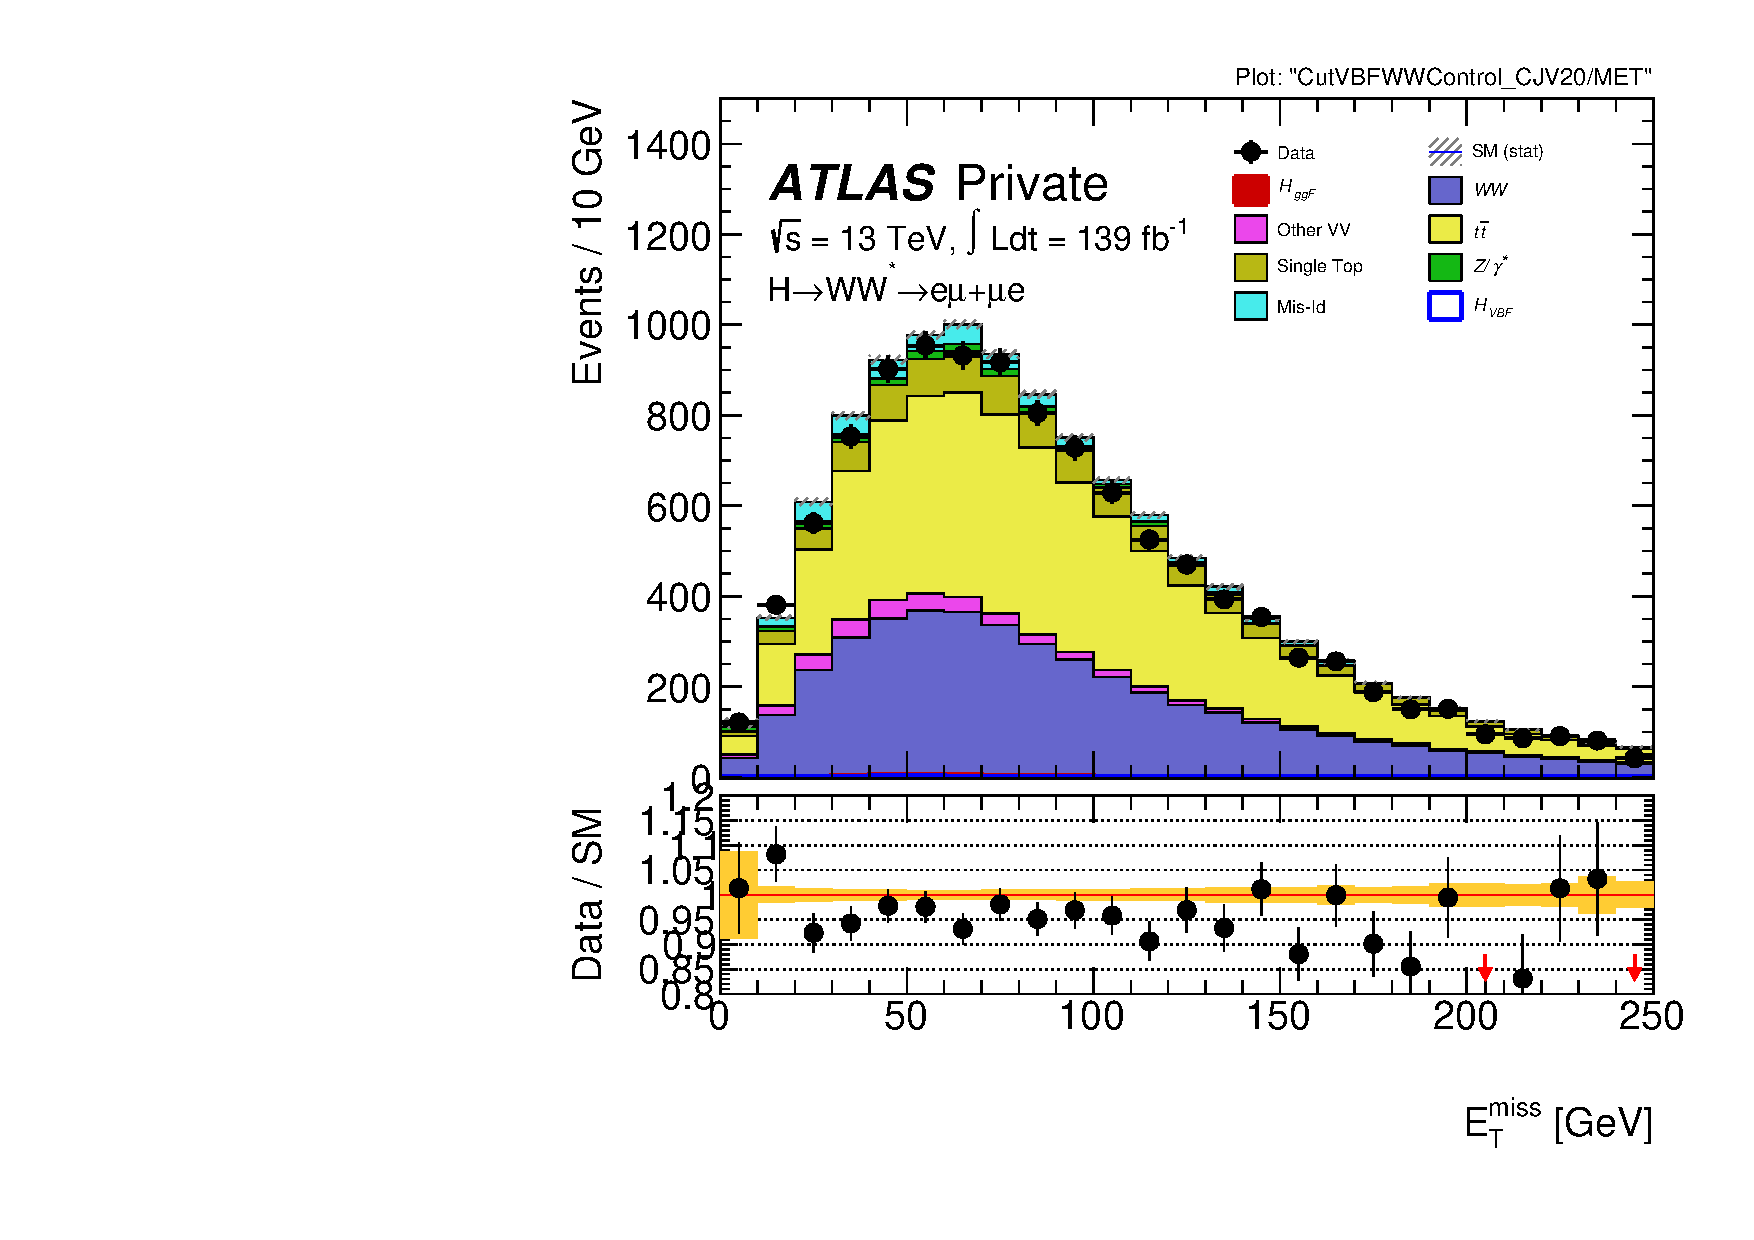
\includegraphics[width=0.3\textwidth]{Pictures/run2-emme-CutVBFWWControl_CJV20-MET-lin.pdf}
%  }%\hfill 
{\caption{Distributions of $\Delta Y_{\ell\ell}$, $\Delta Y_{jj}$, $\sum$ centralities, $M_{l0j0}$, $M_{l1j1}$, $p_T^{j0}$, $\Delta\Phi_{jj}$, $p^T_{tot}$, and $m_T$ in the $WW$ validation region.
\label{fig:WWCR3}}}
\end{figure}

\subsubsection{Top vs. $WW$ BDT discriminant}

This BDT is trained using $e\mu+\mu e$ events after the VBF selection and all signal regions cuts so that the phase space in which we train the BDT is exactly the same as the one where we apply it in the final fit. The training includes weighted samples of top and $WW$ events trained against one another. The MC statistics used in the training are half those available after all signal region cuts where the other half are later used to test the training. This corresponds to $\approx$ 35,000 un-weighted top and and $\approx$ 55,000 raw $WW$ events. This training includes MC weights on events to best account for overall event distributions and there are $\approx$ 1500 total weighted top used in the training and $\approx$ 500 weighted $WW$ events. 

The TMVA BDTG interface is used to train and test the BDT. The optimal parameters were found through a scan of reasonable values and the final set is summarized in Table~\ref{tab:WWBDTparameters}.
\begin{table}[h!]
\centering
\begin{tabular}{|l|c|}
\hline
Parameter                                    & Value     \\
\hline
Boosting algorithm                           &  Gradient  \\
Maximum tree depth                           &  22       \\
Number of trees                              &  200     \\
Minimum number of events requires per mode   &  5\%      \\
Number of cuts                               &  7        \\
\hline
\end{tabular}
\caption{BDT parameters used for the top vs. $WW$ training.} 
\label{tab:WWBDTparameters}
\end{table}

This BDT utilizes a collection of lepton and jet kinematic variables (14) to distinguish between top and $WW$ events. These include $\Delta Y_{jj}$, $\Delta Y_{\ell\ell}$, $\Delta \Phi_{\ell\ell}$, $m_T$, $\eta_{l0}$, $\eta_{l1}$, $p^T_{j0}$, $p^T_{j1}$, $\Delta \Phi_{jj}$, $\sum$ centralities (L), and combined masses $M_{l0j0}$, $M_{l0j1}$, $M_{l1j0}$, $M_{l1j1}$. While a larger variety of variables have been tested, these demonstrated the highest discrimination between top and $WW$ events. Plots shown in \ref{fig:WWBDTinput} and \ref{fig:WWcorrSB} demonstrate the input distributions used to train the BDT and their correlations.
\begin{figure}[!htbp]
    \centering
    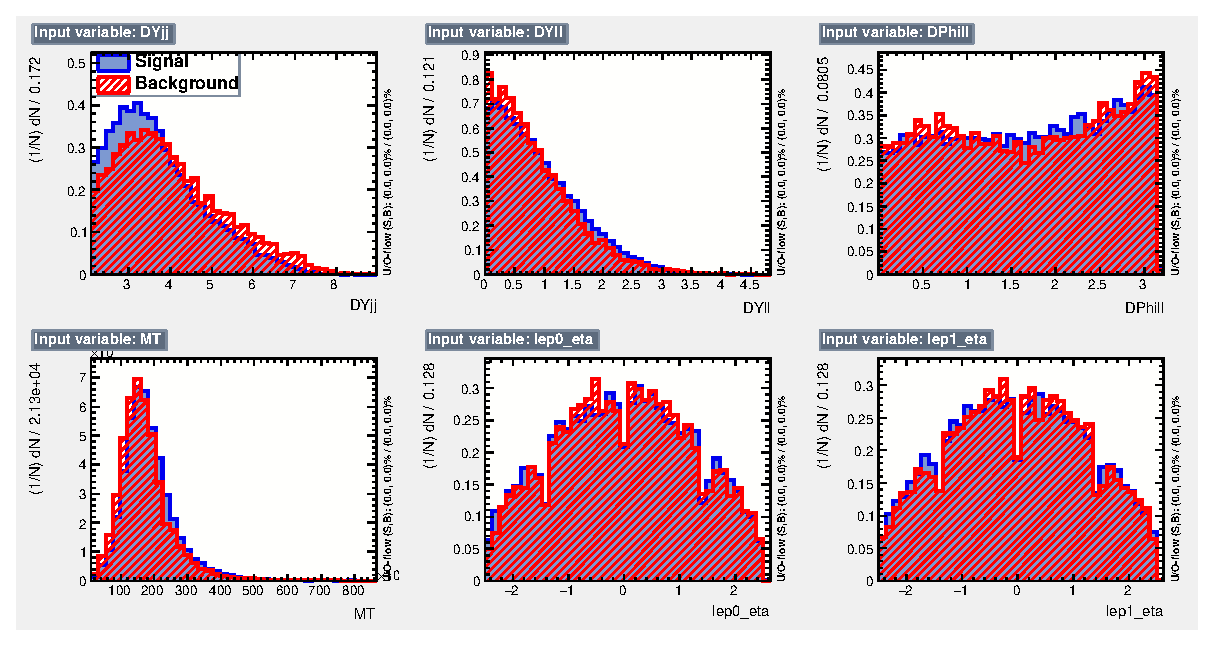
\includegraphics[width=0.45\linewidth]{Pictures/TopvsWW/variables_id_c1.eps}
    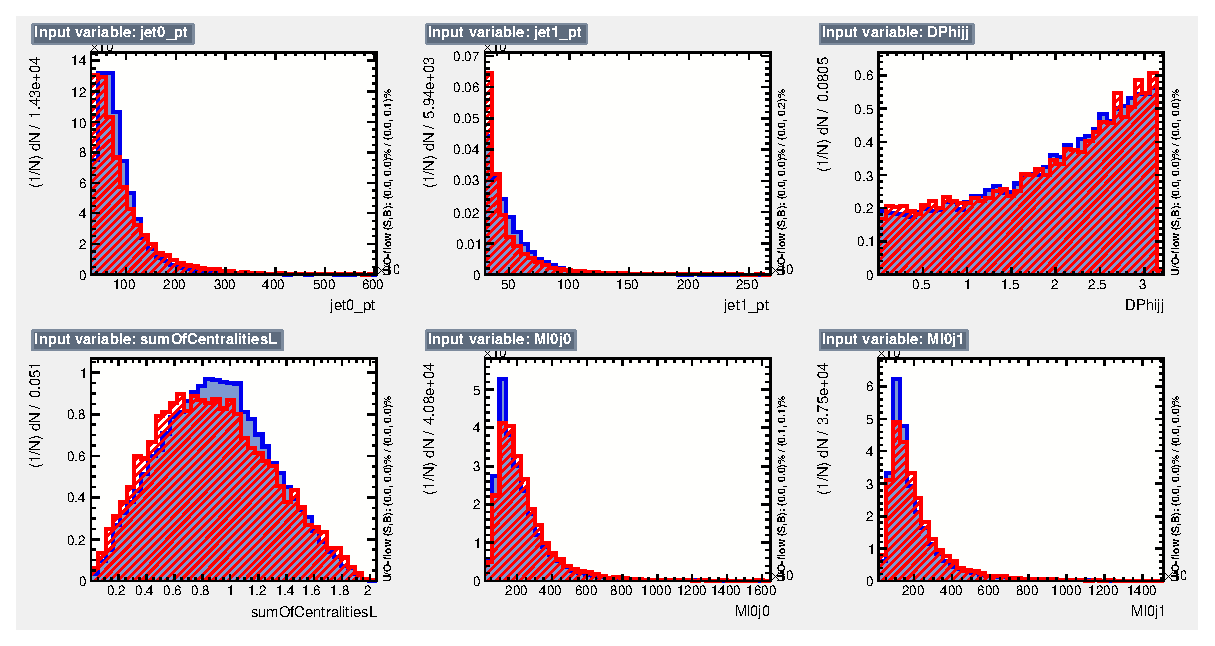
\includegraphics[width=0.45\linewidth]{Pictures/TopvsWW/variables_id_c2.eps}
    \caption{Distributions of input variables to top vs. $WW$ BDT. Samples are weighted and normalized to even numbers of background and signal events. Signal represents top and background $WW$.*}.
    \label{fig:WWBDTinput}
\end{figure}
\begin{figure}[!htbp]
\centering
  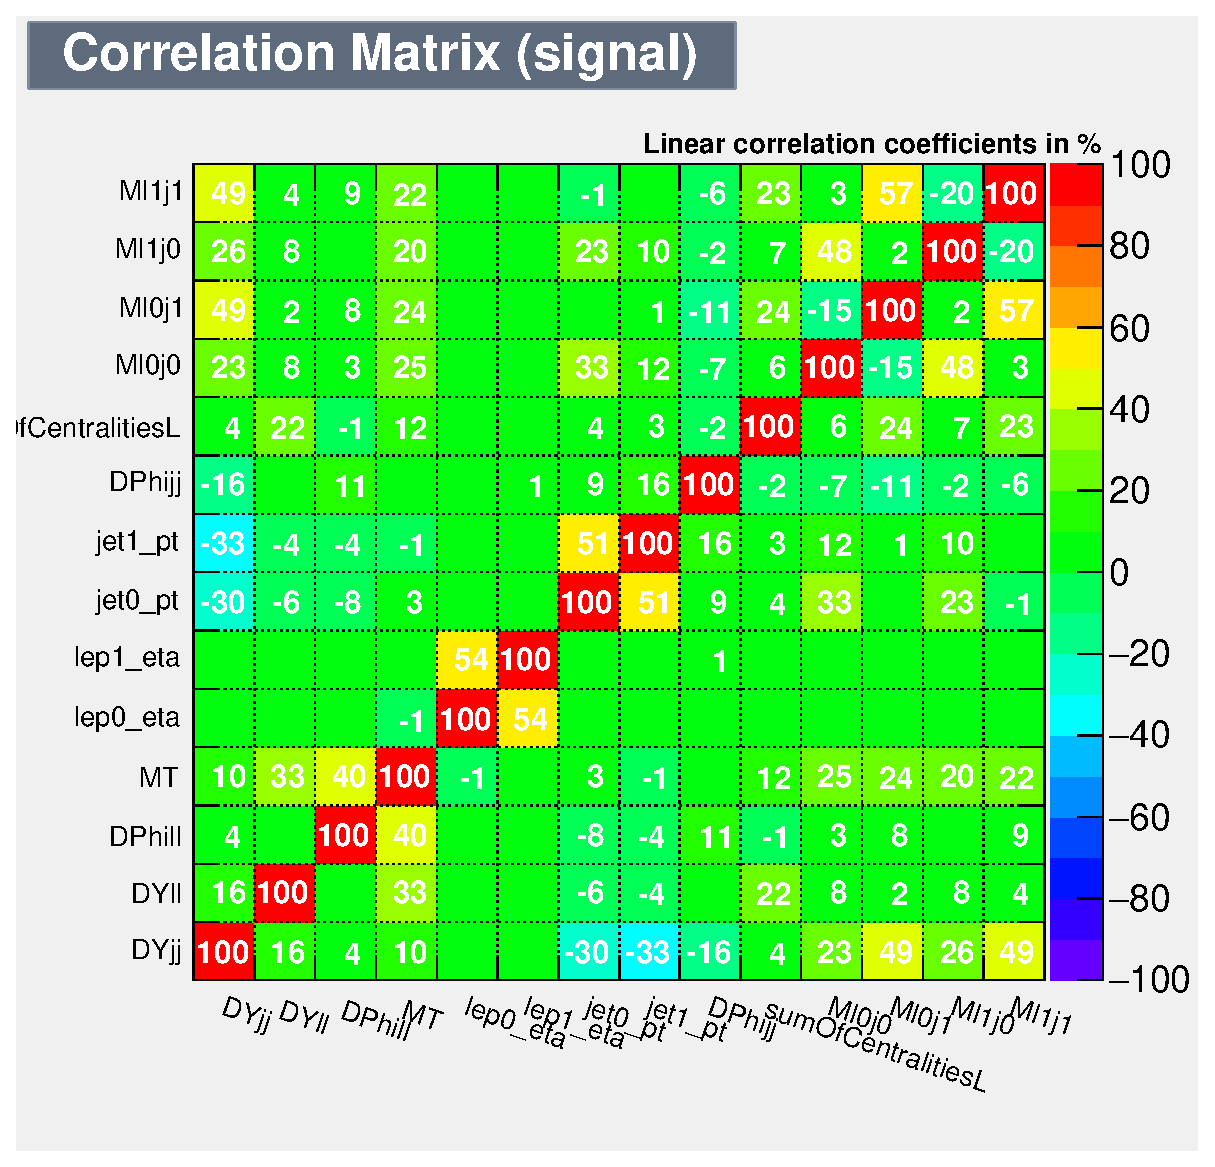
\includegraphics[width=.3\linewidth]{Pictures/TopvsWW/CorrelationMatrixS.eps}
  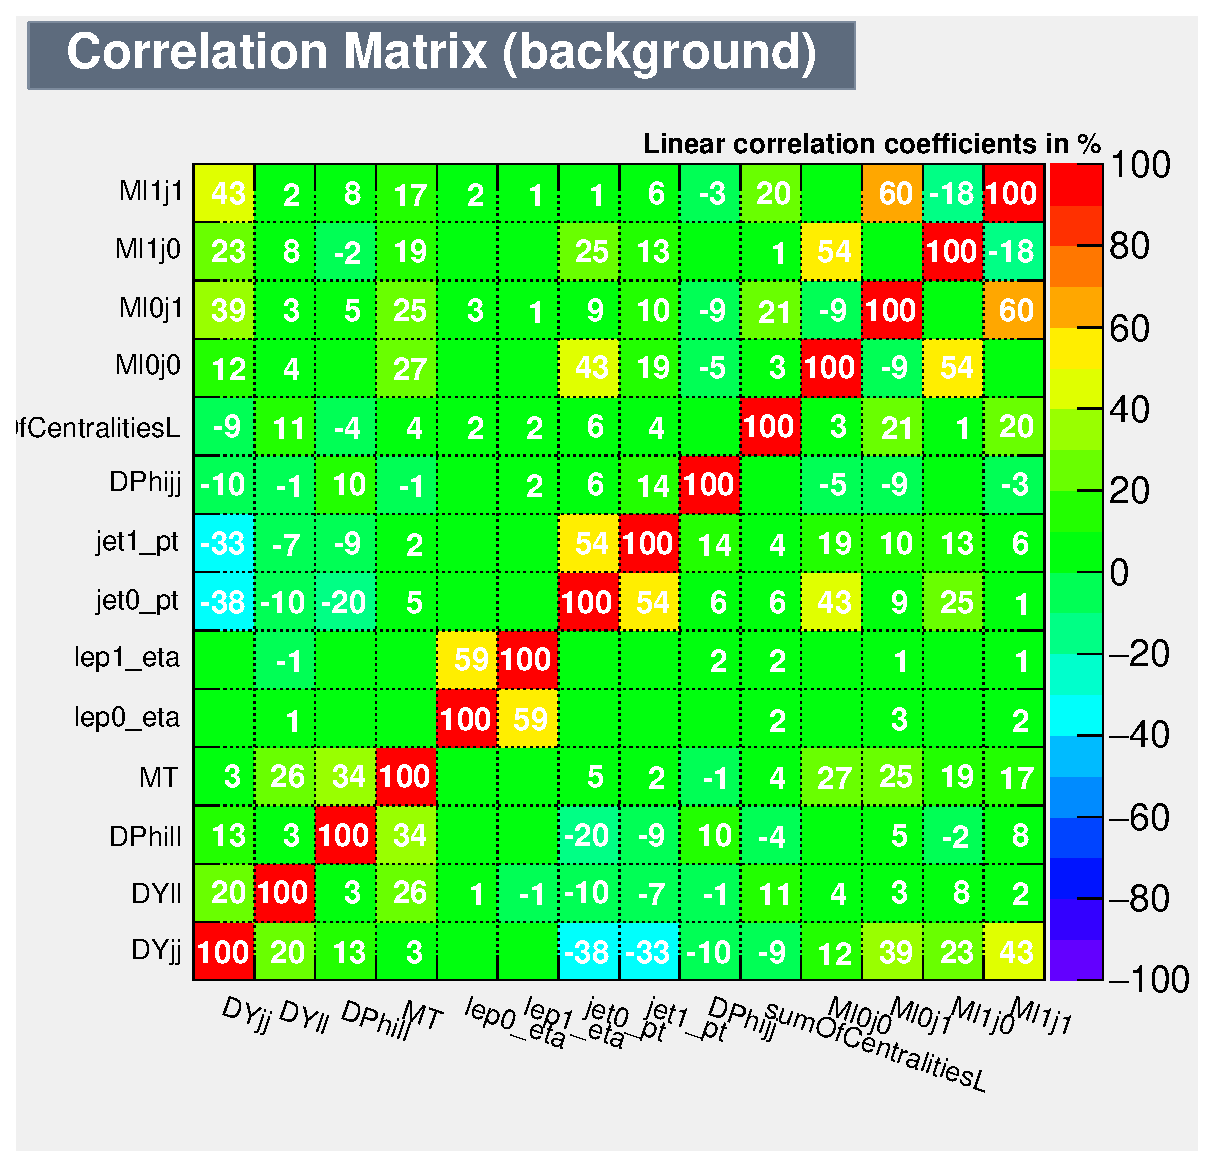
\includegraphics[width=.3\linewidth]{Pictures/TopvsWW/CorrelationMatrixB.eps}
\caption{Correlations of input variables to top vs. $WW$ BDT. Signal represents top and background $WW$*}
\label{fig:WWcorrSB}
\end{figure}
The BDT training separates top and $WW$ backgrounds somewhat. These signals have similar kinematic distributions that make high discrimination difficult. In order to quantify the discrimination we use the integrated-ROC calculated through TMVA for weighted normalized samples and find an optimal value of 0.653. While relatively low, this shows some minimal amount of discrimination. This is useful in the fit to differentiate top and $WW$ backgrounds, though high levels of separation are not necessary because top and $WW$ are estimated together with a shared parameter in the simultaneous fit. Comparisons between the test and training show that the BDT is un-biased. For signal and background we find KS-test values of 0.067 and 0.037, and so no evidence of over-training. We can visualize the BDT output variable both on weighted normalized samples and on samples with all event weights applied. The following plot shows BDT results applied to all samples.

\begin{figure}[!htbp]
\centering
  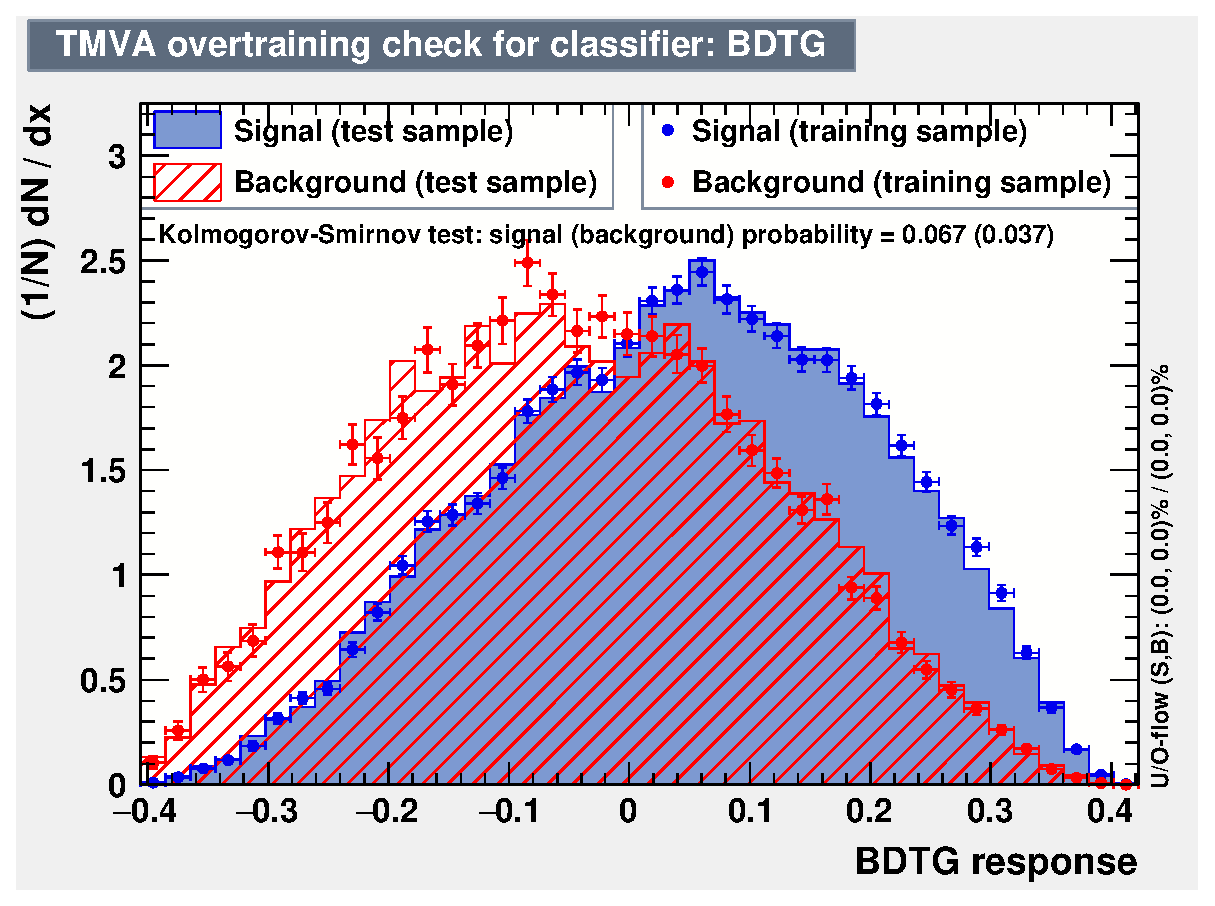
\includegraphics[width=.45\linewidth]{Pictures/TopvsWW/overtrain_BDTG.eps}
  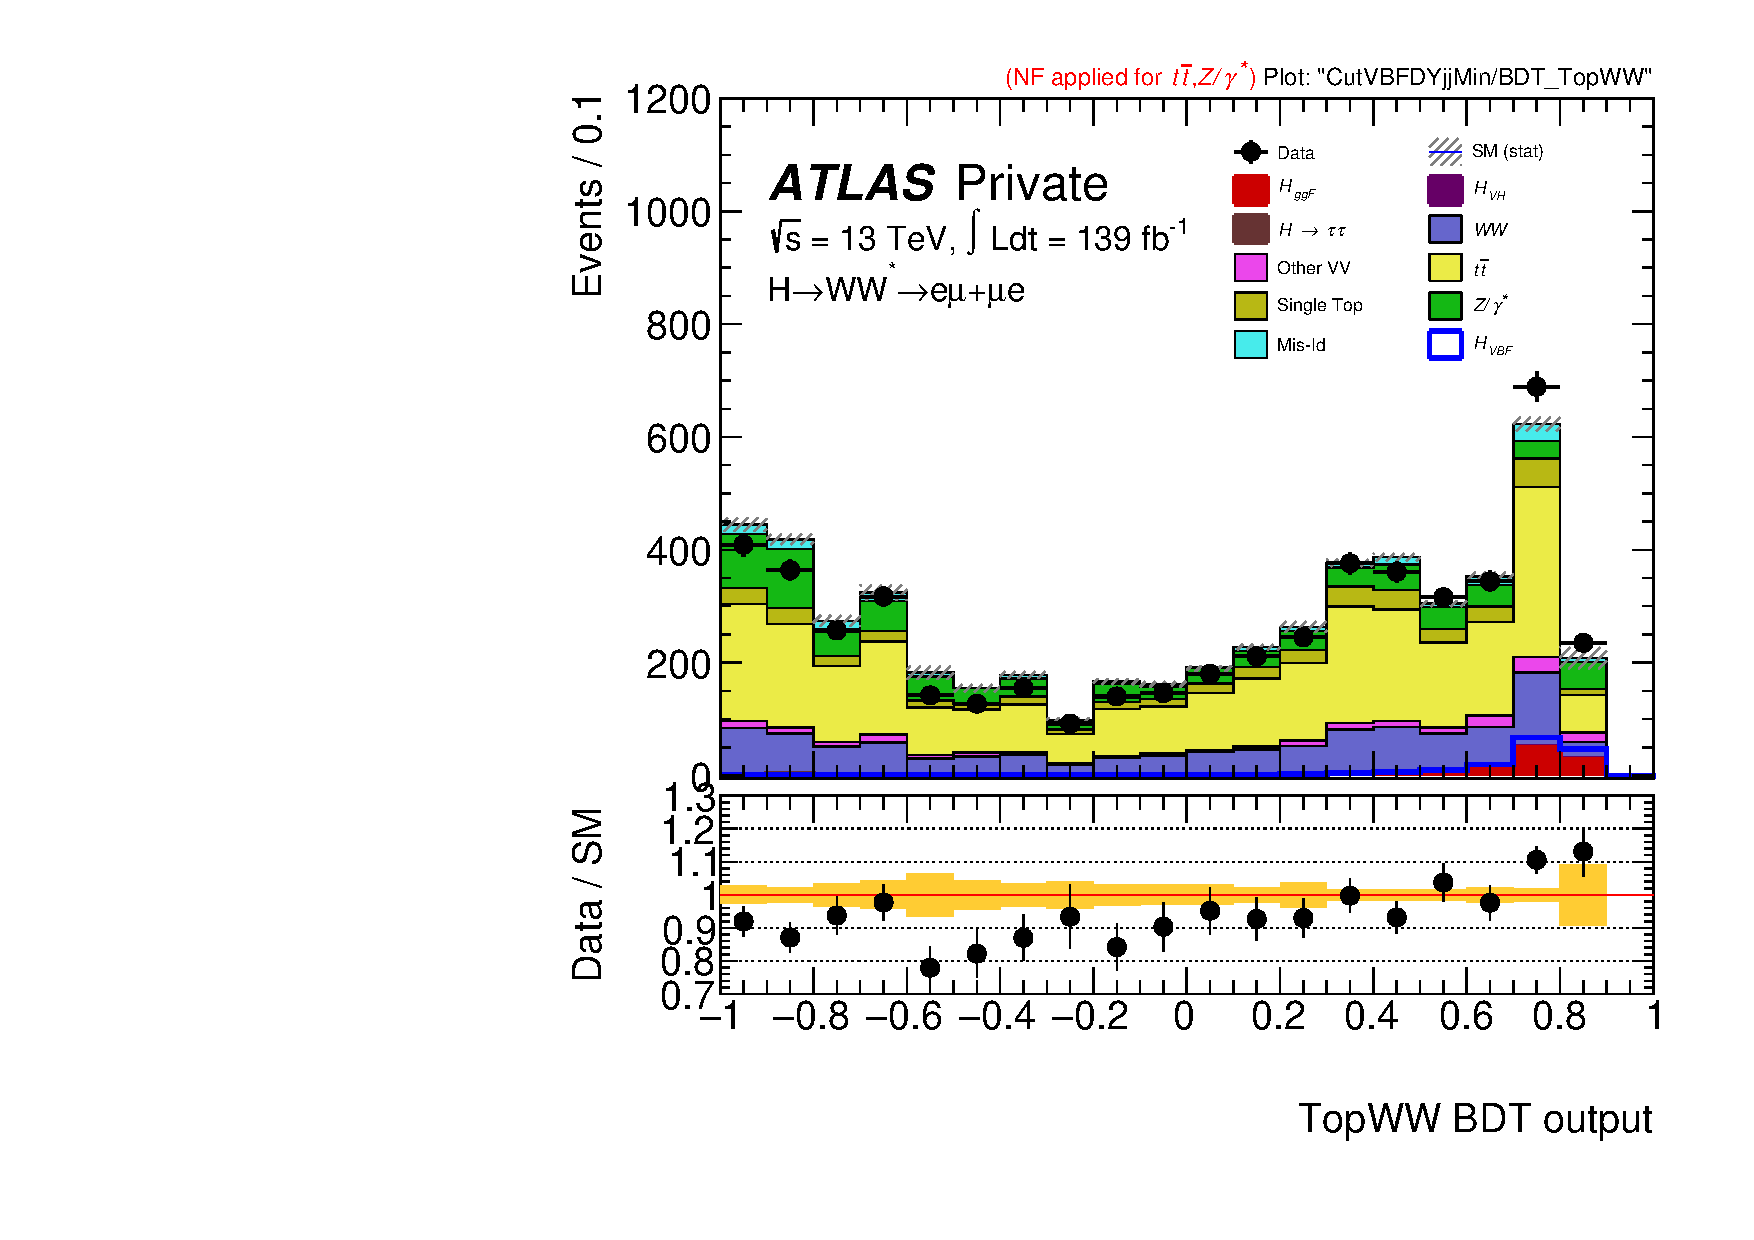
\includegraphics[width=.35\linewidth]{Pictures/run2-emme-CutVBFDYjjMin-BDT_TopWW-lin.pdf}
\caption{Weighted, normalized samples of top samples (signal) and $WW$ samples (background) plotted over BDT output distribution on left, overlaid testing and training samples shown. Right, full weighted samples of all signal and background events plotted over the BDT output distribution after signal region selection. Data is blinded here*}
\label{fig:WWBDTresult}
\end{figure}

We aim to fit this distribution in the signal region with high significance for top events in uppermost bins of the distribution (and $WW$ in the lowermost). Since this BDT is trained and applied in the signal region we cannot directly test the modelling of input variables. However, modelling at the pre-selection level for each of these variables as well as in the $WW$ validation region described eariler show no evidence of mis-modelling. The binning for this discriminant used in the statistical fit and its result (using Asimov data) are shown in the final chapter. We can visualize this BDT discriminant in the $WW$ validation region to gain an idea of overall modelling particularly of the $WW$ events.

\begin{figure}[!htbp]
\centering
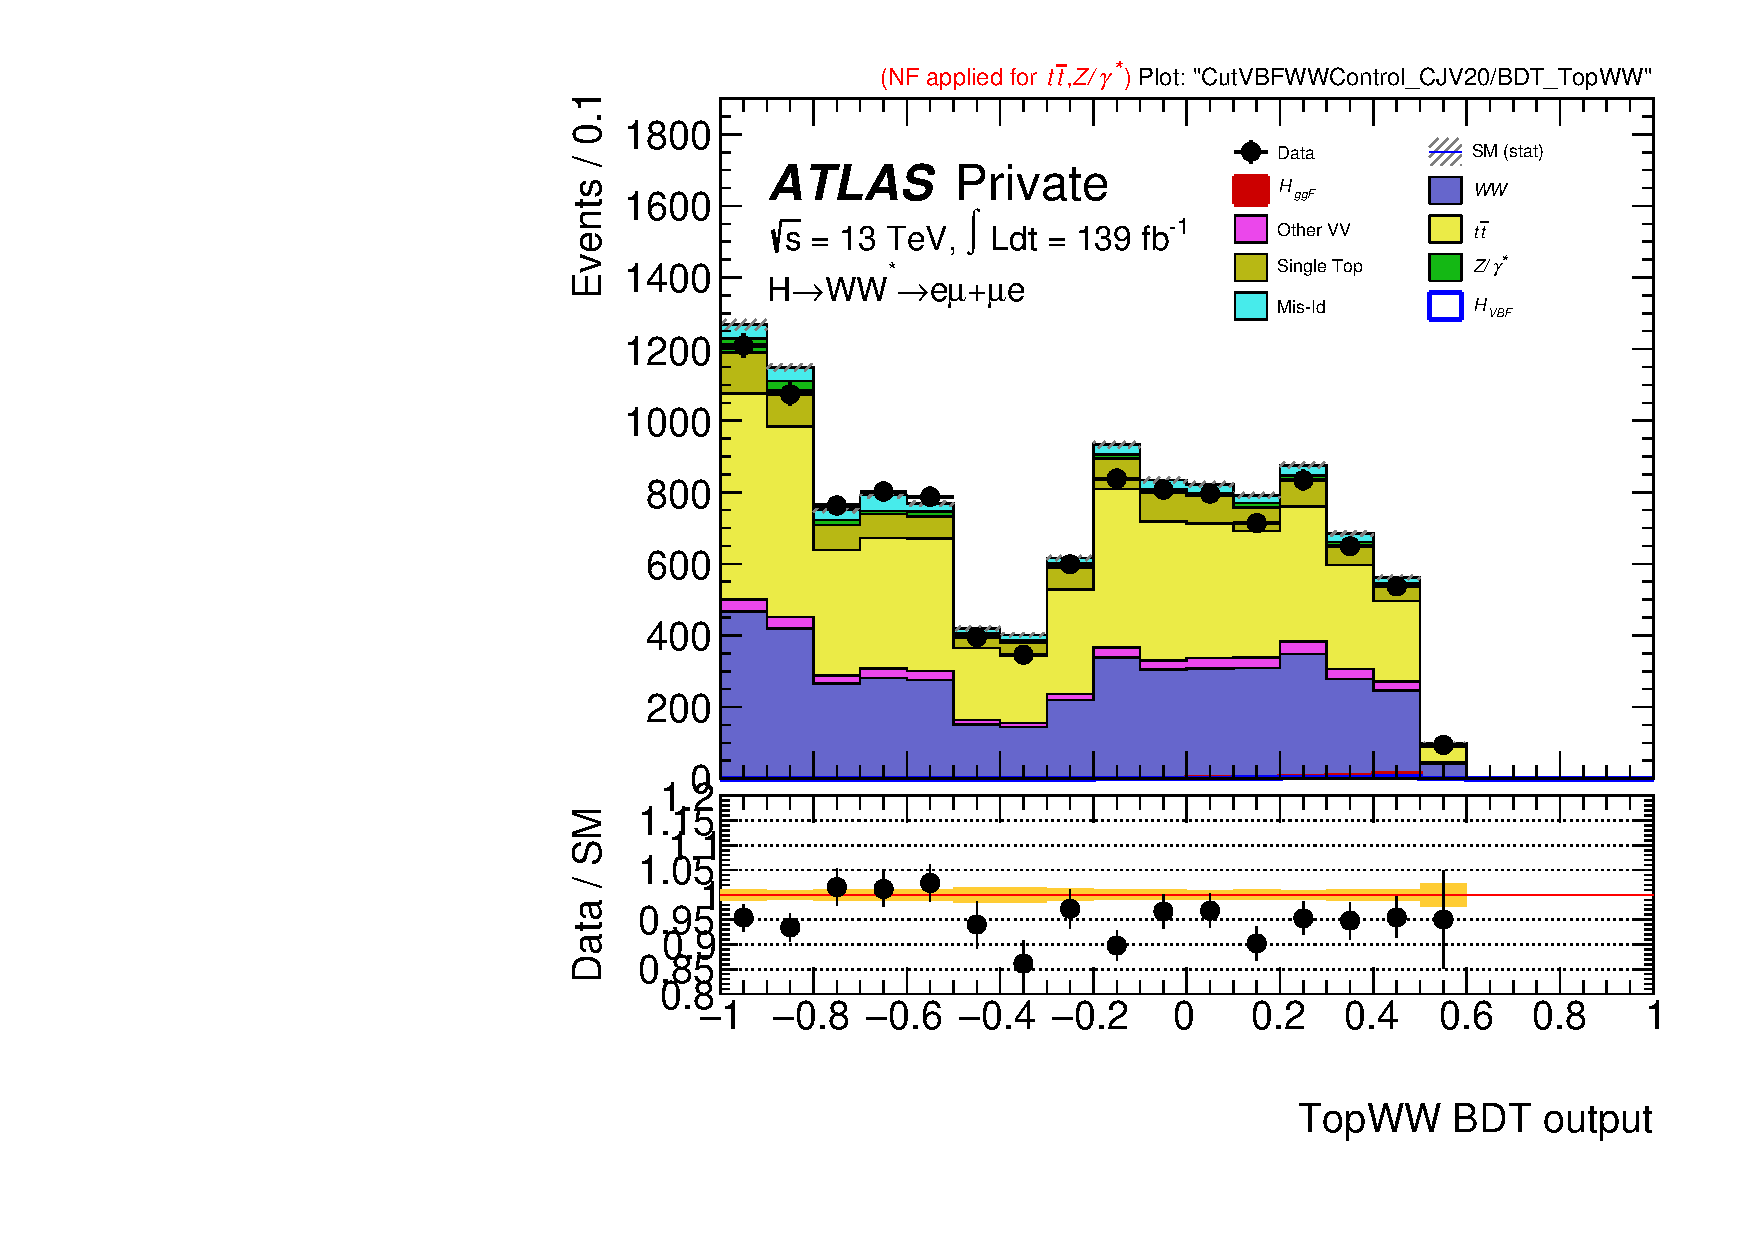
\includegraphics[width=.4\linewidth]{Pictures/run2-emme-CutVBFWWControl_CJV20-BDT_TopWW-lin.pdf}
\caption{Full weighted samples of all signal and background plotted over BDT output distributions in $WW$ validation region}
\label{fig:TopvWWBDTVR}
\end{figure}

The BDT to discriminate top$+WW$ background from VBF, ggF, $Z+$jets and $V\gamma$ events is trained and applied in the signal region and described in the previously, but its distribution in the $WW$ validation region is also shown. 

\begin{figure}[!htbp]
\centering
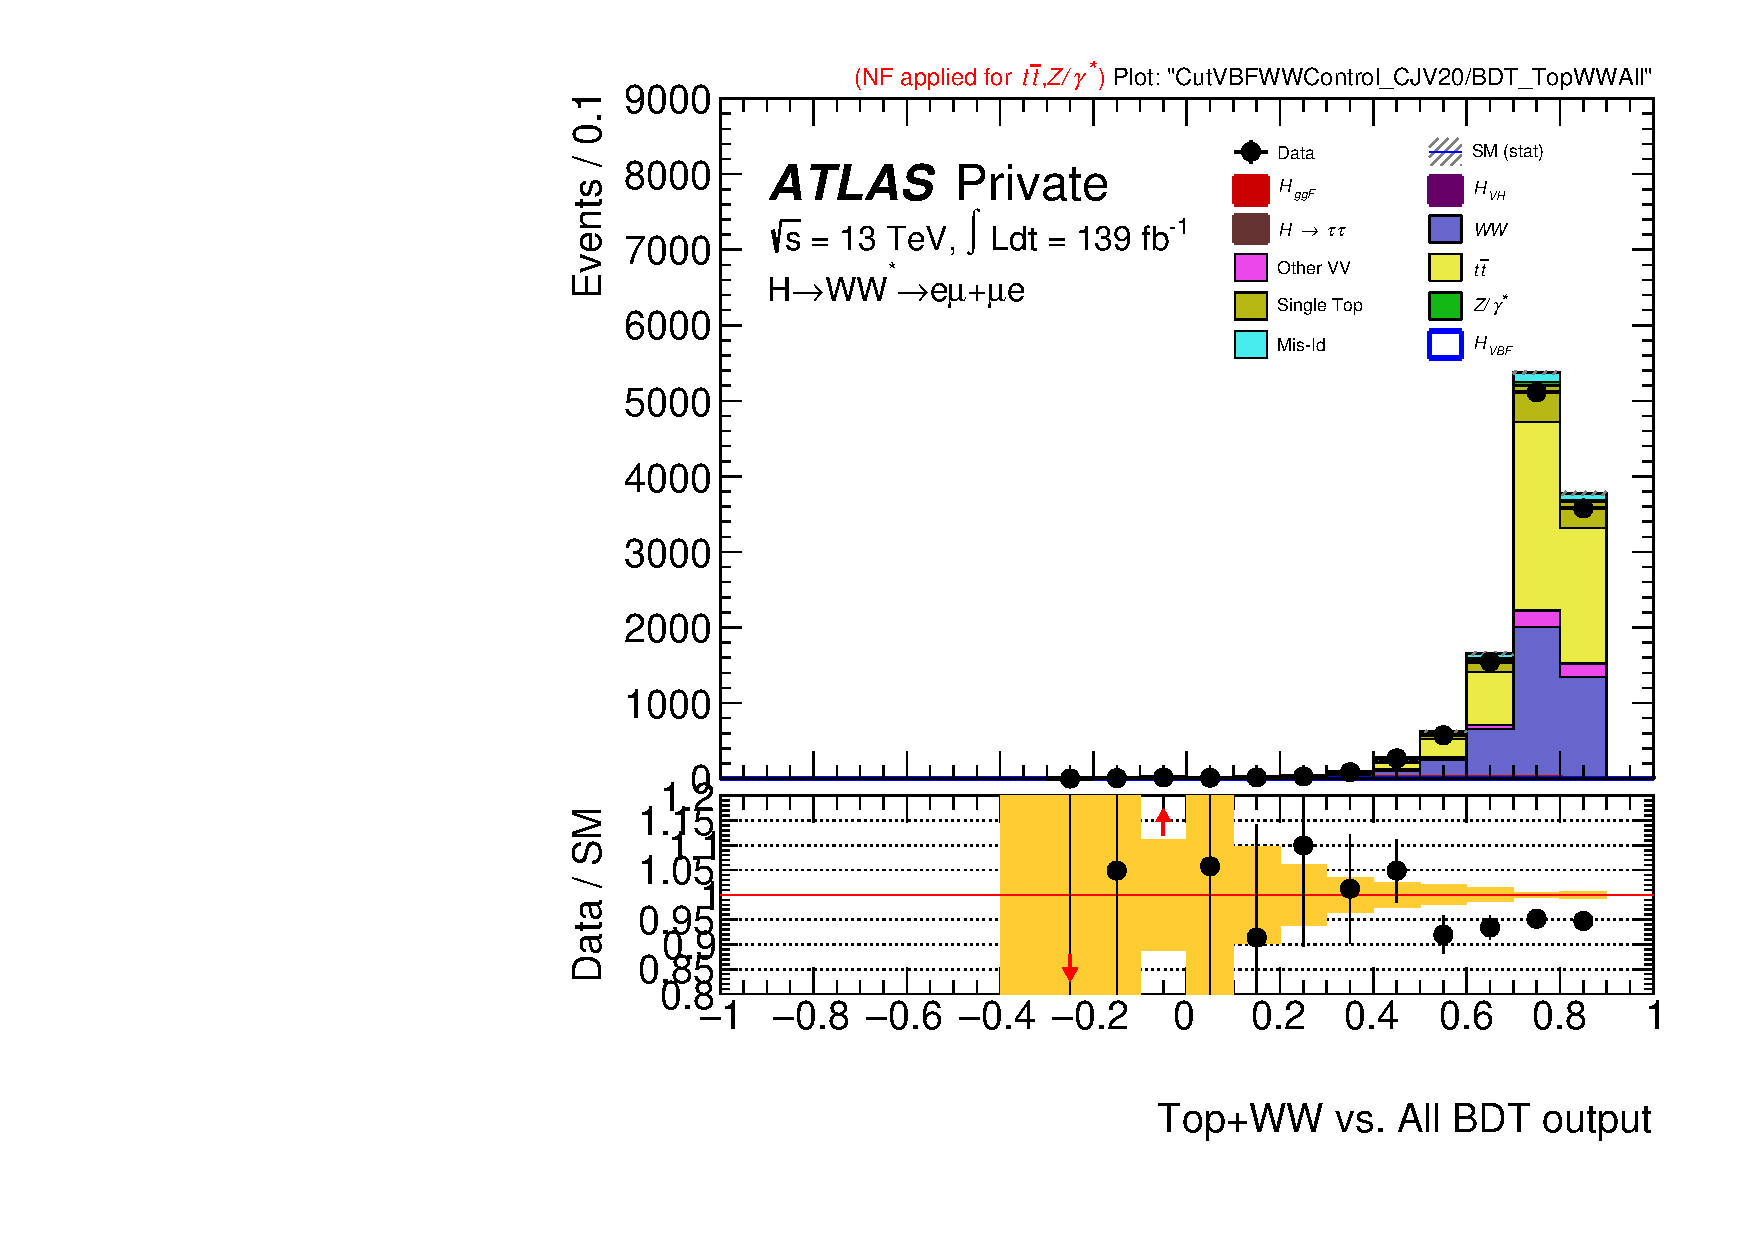
\includegraphics[width=.4\linewidth]{Pictures/run2-emme-CutVBFWWControl_CJV20-BDT_TopWWAll-lin.pdf}
\caption{Full weighted samples of all signal and background plotted over Top + $WW$ vs. VBF ggF + $Z+$jets +$V\gamma$ BDT output distributions in $WW$ validation region}
\label{fig:TopvWWBDTVR}
\end{figure}

The BDT to discriminate $WW$ background from VBF signal events is trained and applied in the signal region and so described in the previous chapter, but its distribution in the $WW$ validation region is shown below. This BDT discriminates both WW and top (combined) against the VBF signal as they have similar kinematic distributions and are treated together in the final simultaneous fit.

\begin{figure}[!htbp]
\centering
\includegraphics[width=.4\linewidth]{Pictures/run2-emme-CutVBFWWControl_CJV20-BDT_VBF-lin.pdf}
\caption{Full weighted samples of all signal and background plotted over Top + $WW$ vs. VBF BDT output distributions in $WW$ validation region}
\label{fig:VBFvWWTopBDTVR}
\end{figure}

\subsection{ggF background}
Other Higgs productions modes are considered backgrounds in this analysis- and while vector mediated Higgs production ($VH$) and top produced Higgs ($ttH$) are small in our signal region so don't play a large role in the analysis - gluon fusion Higgs production (ggF) represents a significant background. Signal region cuts requiring at least 2-jets and the central jet veto significantly reduce background yields, but because it is kinematically very similar to VBF signal, it has a large effect on the VBF differential coupling measurement. To mitigate these effects, ggF events are simultaneously estimated from three control regions and the signal region. The control regions are chosen to minimize both the statistical and the modelling uncertainties, in particular those originating from the modelling of higher order QCD corrections. The regions begin with a subdivision based on the jet multiplicity. The first two regions, ggF CR1 and ggF CR2, are built from all preselection cuts and cuts requiring at least two jets, a $b$-veto, $Z\rightarrow\tau\tau$-veto, and orthogonal cuts on the central jet veto (CJV) and opposite lepton veto (OLV). The third ggF control region, ggF CR3, uses all preselection cuts, a $b$ veto, $Z\rightarrow \tau\tau$ veto, and requirement for less than 2 jets. The full definitions are described:  
\begin{itemize} 
\item {\textbf GGF-CR1} Preselection criteria and $N_{ \text{jet}}>=2$, $b$ veto, $Z\rightarrow\tau\tau$ veto, $\text{CJV}<1$ and $\text{OLV}>1$ or $\text{CJV}>1$ and $\text{OLV}<1$.
\item {\textbf GGF-CR2} Preselection criteria and $N_{ \text{jet}}>=2$, $b$ veto, $Z\rightarrow\tau\tau$ veto, $\text{CJV} > 1$ and $\text{OLV} > 1$. 
\item {\textbf GGF-CR3} Preselection criteria and $N_{ \text{jet}}>=2$, $b$ veto, and $Z\rightarrow\tau\tau$ veto. 
\end{itemize} 
The full ggF expectation in the signal region is built from the following ratio (inspired by the ABCD method) 
\begin{equation}
	\mu_{{\text GGF-SR}} = \frac{\mu^{{\text GGF-CR}}_{3} \cdot\mu^{{\text GGF-CR}}_{1}}{ \mu^{{\text GGF-CR}}_{2}}.
\end{equation}
where $\mu_{\text{ggF-X}}$ represents the yield modifier in each ggF control region. The final event yield in the signal region $\mu_{{\text ggF-SR}}$ is determined in the simultaneous fit as described in the next chapter. In each ggF category the ggF yield is extracted from simulation-extracted template fits based on dedicated discriminants. For each control region a dedicated multivariate discriminant is trained and applied to discriminate between ggF and all the backgrounds combined. Results and training parameters from each of these discriminants is summarized next.

\subsubsection{Discriminant in ggF CR1}
The multivariate discriminant used for the ggF CR1 is a boosted decision tree (BDT) trained using $e\mu+\mu e$ events that pass all ggF CR1 cuts. The training includes ggF events trained against VBF signal and all backgrounds. The MC statistics used in the training are half those available after the ggF CR1 cuts (as the other half are later used to test the training). This corresponds to $\approx$ 8,000 ggF events and $\approx$250,000 other signal and background events. Events are trained with MC weights applied to accurately represent relative importance of each event and the training uses $\approx$ 130 weighted ggF samples and $\approx$ 10,000 weighted other background samples.  

The TMVA BDTG interface is used to train and test the BDT. The optimal parameters were found through a scan of reasonable values and the final set is summarized in Table~\ref{tab:ggFCR1BDTparameters}.
\begin{table}[h!]
\centering
\begin{tabular}{|l|c|c|}
\hline
Parameter                                    & Value     \\
\hline
Boosting algorithm                           & Gradient \\
Maximum tree depth                           &  10      \\
Number of trees                              &  600    \\
Minimum number of events requires per mode   &  5\%     \\ 
Number of cuts                               &  7       \\
\hline
\end{tabular}
\caption{BDT parameters used for the ggF CR1 training.}
\label{tab:ggFCR1BDTparameters}
\end{table}
For this BDT various distributions (8) are used to take advantage of differences in distributions between ggF events and other sample types. These variables include $\Delta Y_{\ell\ell}$, $\Delta \Phi_{\ell\ell}$,$m_{\ell\ell}$,$m_T$, jet $p^T_{\text{lead}}$, jet $p^T_{\text{sublead}}$, $\Delta \Phi_{jj}$, and $\ensuremath{E_{\text{T}}^{\text{miss}}}$. Distributions for these variables in the ggF CR1 region where the BDT is trained are shown below demonstrating data/MC modelling for each.
\begin{figure}[!h]
  \subfloat[$\Delta Y_{\ell\ell}$]{
      \includegraphics[width=0.3\textwidth]{Pictures/run2-emme-CutVBFggFCR1-DYll-lin.pdf}
  }\hfill
  \subfloat[$\Delta \Phi_{\ell\ell}$]{
      \includegraphics[width=0.3\textwidth]{Pictures/run2-emme-CutVBFggFCR1-DPhill-lin.pdf}
  }\hfill
  \subfloat[$m_{\ell\ell}$]{
      \includegraphics[width=0.3\textwidth]{Pictures/run2-emme-CutVBFggFCR1-Mll-lin.pdf}
  }\hfill
  \subfloat[$m_T$]{
      \includegraphics[width=0.3\textwidth]{Pictures/run2-emme-CutVBFggFCR1-MT-lin.pdf}
  }\hfill
  \subfloat[jet $p^T_{\text{lead}}$]{
      \includegraphics[width=0.3\textwidth]{Pictures/run2-emme-CutVBFggFCR1-leadJetPt-lin.pdf}
  }\hfill
  \subfloat[jet $p^T_{\text{sublead}}$]{
      \includegraphics[width=0.3\textwidth]{Pictures/run2-emme-CutVBFggFCR1-subleadJetPt-lin.pdf}
  }\hfill
  \subfloat[$\Delta \Phi_{jj}$]{
      \includegraphics[width=0.3\textwidth]{Pictures/run2-emme-CutVBFggFCR1-DPhijj-lin.pdf}
  }\hfill
  \subfloat[$\ensuremath{E_{\text{T}}^{\text{miss}}}$]{
      \includegraphics[width=0.3\textwidth]{Pictures/run2-emme-CutVBFggFCR1-MET-lin.pdf}
  }%\hfill
{\caption{Distributions of $\Delta Y_{\ell\ell}$, $\Delta \Phi_{\ell\ell}$,$m_{\ell\ell}$,$m_T$, jet $p^T_{\text{lead}}$, jet $p^T_{\text{sublead}}$, $\Delta \Phi_{jj}$, and $\ensuremath{E_{\text{T}}^{\text{miss}}}$ in the ggF CR1 used as input to the BDT discriminating ggF from all other samples.
\label{fig:ggFCR1}}}
\end{figure} 

Plots shown in \ref{fig:ggFCR1BDTinput} and \ref{fig:ggFCR1corrSB} demonstrate the input distributions used to train the BDT and their correlations where each distribution is normalized to equal number of background and signal events. 

\begin{figure}[!htbp]
    \centering
    \includegraphics[width=0.45\linewidth]{Pictures/ggFCR1/variables_id_c1.eps}
    \includegraphics[width=0.45\linewidth]{Pictures/ggFCR1/variables_id_c2.eps}
    \caption{Distributions of input variables to ggF CR1 BDT. Samples are weighted and normalized to even numbers of background and signal events. Signal represents ggF and background all other samples.*}.
    \label{fig:ggFCR1BDTinput}
\end{figure}
\begin{figure}[!htbp]
\centering
  \includegraphics[width=.3\linewidth]{Pictures/ggFCR1/CorrelationMatrixS.eps}
  \includegraphics[width=.3\linewidth]{Pictures/ggFCR1/CorrelationMatrixB.eps}
\caption{Correlations of input variables to ggF CR1 BDT. Signal represents ggF and background all other samples.*}
\label{fig:ggFCR1corrSB}
\end{figure}

In order to quantify the discrimination we use the integrated-ROC calculated through TMVA for weighted normalized samples and find an optimal value of 0.898. Comparisons between the test and training show that the BDT is un-biased- differences between testing and training samples would imply overtraining, or the BDT using too many parameters on too few events. Visually, we can see that the testing and trainings samples are quite similar. Additionally, a Kolmogorov-Smirnov test is performed to measure if the two test and training distributions differ significantly and no evidence of over-training is present (values 0.191, 0.049 for signal, background). We can visualize the BDT output variable both on weighted normalized samples and on samples without normalization. The following plots show BDT results applied to normalized and full weighted samples.

\begin{figure}[!htbp]
\centering
  \includegraphics[width=.4\linewidth]{Pictures/ggFCR1/overtrain_BDTG.eps}
  \includegraphics[width=.45\linewidth]{Pictures/run2-emme-CutVBFggFCR1-BDT_ggFCR1-log.pdf}
\caption{Normalized samples of ggF (signal) and all other samples (background) plotted over BDT output distribution on left, overlaid testing and training samples shown. Right, full weighted samples of ggF signal and all other backgrounds plotted over BDT output distribution after ggF CR 1.*}
\label{fig:ggFCR1BDTresult}
\end{figure}

\subsubsection{Discriminant in ggF CR2}

The multivariate discriminant used for ggF CR2 is a boosted decision tree trained using $e\mu+\mu e$ events that pass all ggF CR2 cuts. The training includes ggF events trained against VBF signal and all backgrounds. The MC statistics used in the training are half those available after ggF CR2 cuts (as the other half are later used to test the training). This corresponds to $\approx$ 22,200 ggF events and $\approx$90,000 other signal and background events.

The TMVA BDTG interface is used to train and test the BDT. The optimal parameters were found through a scan of reasonable values and the final set is summarized in Table~\ref{tab:ggFCR2BDTparameters}.
\begin{table}[h!]
\centering
\begin{tabular}{|l|c|c|}
\hline
Parameter                                    & Value     \\
\hline
Boosting algorithm                           & Gradient \\
Maximum tree depth                           &  10      \\
Number of trees                              &  50    \\
Minimum number of events requires per mode   &  5\%     \\ 
Number of cuts                               &  7       \\
\hline
\end{tabular}
\caption{BDT parameters used for the ggF CR2 training.}
\label{tab:ggFCR2BDTparameters}
\end{table}
For this BDT various distributions (6) are used to take advantage of differences in distributions between ggF events and other sample types. These variables include $\Delta Y_{\ell\ell}$, $\Delta \Phi_{\ell\ell}$,$m_{\ell\ell}$,$m_T$, $\Delta \Phi_{jj}$, and $\ensuremath{E_{\text{T}}^{\text{miss}}}$. Distributions for these variables in the ggF CR2 region where the BDT is trained are shown below demonstrating data/MC modelling for each.
\begin{figure}[!h]
  \subfloat[$\Delta Y_{\ell\ell}$]{
      \includegraphics[width=0.3\textwidth]{Pictures/run2-emme-CutVBFggFCR2-DYll-lin.pdf}
  }\hfill
  \subfloat[$\Delta \Phi_{\ell\ell}$]{
      \includegraphics[width=0.3\textwidth]{Pictures/run2-emme-CutVBFggFCR2-DPhill-lin.pdf}
  }\hfill
  \subfloat[$m_{\ell\ell}$]{
      \includegraphics[width=0.3\textwidth]{Pictures/run2-emme-CutVBFggFCR2-Mll-lin.pdf}
  }\hfill
  \subfloat[$m_T$]{
      \includegraphics[width=0.3\textwidth]{Pictures/run2-emme-CutVBFggFCR2-MT-lin.pdf}
  }\hfill
%  \subfloat[$p^T_{tot}$]{
%      \includegraphics[width=0.3\textwidth]{Pictures/run2-emme-CutVBFggFCR2-PtTot-lin.pdf}
%  }\hfill
%  \subfloat[lep $p^T_{\text{lead}}$]{
%      \includegraphics[width=0.3\textwidth]{Pictures/run2-emme-CutVBFggFCR2-leadLepPt-lin.pdf}
%  }\hfill
%  \subfloat[jet $p^T_{\text{lead}}$]{
%      \includegraphics[width=0.3\textwidth]{Pictures/run2-emme-CutVBFggFCR2-leadJetPt-lin.pdf}
%  }\hfill
%  \subfloat[lep $p^T_{\text{sublead}}$]{
%      \includegraphics[width=0.3\textwidth]{Pictures/run2-emme-CutVBFggFCR2-subleadLepPt-lin.pdf}
%  }\hfill
%  \subfloat[jet $p^T_{\text{sublead}}$]{
%      \includegraphics[width=0.3\textwidth]{Pictures/run2-emme-CutVBFggFCR2-subleadJetPt-lin.pdf}
%  }\hfill
  \subfloat[$\Delta \Phi_{jj}$]{
      \includegraphics[width=0.3\textwidth]{Pictures/run2-emme-CutVBFggFCR2-DPhijj-lin.pdf}
  }\hfill
  \subfloat[$\ensuremath{E_{\text{T}}^{\text{miss}}}$]{
      \includegraphics[width=0.3\textwidth]{Pictures/run2-emme-CutVBFggFCR2-MET-lin.pdf}
  }%\hfill
{\caption{Distributions of $\Delta Y_{\ell\ell}$, $\Delta \Phi_{\ell\ell}$,$m_{\ell\ell}$,$m_T$, $\Delta \Phi_{jj}$, and $\ensuremath{E_{\text{T}}^{\text{miss}}}$ in the ggF CR2 used as input to the BDT discriminating ggF from all other samples.
\label{fig:ggFCR2}}}
\end{figure} 

Plots shown in \ref{fig:ggFCR2BDTinput} and \ref{fig:ggFCR2corrSB} demonstrate the input distributions used to train the BDT and their correlations where each distribution is weighted and normalized to equal number of background and signal events. 

\begin{figure}[!htbp]
    \centering
    \includegraphics[width=0.5\linewidth]{Pictures/ggFCR2/variables_id_c1.eps}
    \caption{Distributions of input variables to ggF CR2 BDT. Samples are weighted and normalized to even numbers of background and signal events. Signal represents ggF and background all other samples.*}.
    \label{fig:ggFCR2BDTinput}
\end{figure}
\begin{figure}[!htbp]
\centering
  \includegraphics[width=.3\linewidth]{Pictures/ggFCR2/CorrelationMatrixS.eps}
  \includegraphics[width=.3\linewidth]{Pictures/ggFCR2/CorrelationMatrixB.eps}
\caption{Correlations of input variables to ggF CR2 BDT. Signal represents ggF and background all other samples.*}
\label{fig:ggFCR2corrSB}
\end{figure}

In order to quantify the discrimination we use the integrated-ROC calculated through TMVA for weighted normalized samples and find an optimal value of 0.902. Comparisons between the test and training show that the BDT is un-biased- visually, once can see that the testing and trainings samples are quite similar. Additionally, a Kolmogorov-Smirnov test is performed to measure if the two test and training distributions differ significantly and with values of 0.012 (0.303) for signal (background) no evidence of over-training is present. We can visualize the BDT output variable both on weighted normalized samples and on samples with full event weights applied. The following plots show BDT results applied to normalized and full weighted samples.

\begin{figure}[!htbp]
\centering
  \includegraphics[width=.4\linewidth]{Pictures/ggFCR2/overtrain_BDTG.eps}
  \includegraphics[width=.45\linewidth]{Pictures/run2-emme-CutVBFggFCR2-BDT_ggFCR2-log.pdf}
\caption{Weighted, normalized samples of ggF (signal) and all other samples (background) plotted over BDT output distribution on left, overlaid testing and training samples shown. Right, full weighted samples of ggF signal and all other backgrounds plotted over BDT output distribution after ggF CR2 cuts.*}
\label{fig:ggFCR2BDTresult}
\end{figure}

\subsubsection{Discriminant in ggF-CR3}

The multivariate discriminant used for the ggF CR3 is a boosted decision tree trained using $e\mu+\mu e$ events that pass all ggF CR3 cuts. The training includes only ggF events trained against VBF signal and all backgrounds. The MC statistics used in the training are half those available after the ggF CR3 cuts (as the other half are later used to test the training). This corresponds to $\approx$ 200,000 ggF events and $\approx$2,800,000 other signal and background events.

The TMVA BDTG interface is used to train and test the BDT. The optimal parameters were found through a scan of reasonable values and the final set is summarized in Table~\ref{tab:ggFCR3BDTparameters}.
\begin{table}[h!]
\centering
\begin{tabular}{|l|c|c|}
\hline
Parameter                                    & Value     \\
\hline
Boosting algorithm                           & Gradient \\
Maximum tree depth                           &  10      \\
Number of trees                              &  1000    \\
Minimum number of events requires per mode   &  5\%     \\ 
Number of cuts                               &  7       \\
\hline
\end{tabular}
\caption{BDT parameters used for the ggF CR3 training.}
\label{tab:ggFCR3BDTparameters}
\end{table}
For this BDT various distributions (4) are used to take advantage of differences in distributions between ggF events and other samples types. These variables include $\Delta Y_{\ell\ell}$, $\Delta \Phi_{\ell\ell}$,$m_{\ell\ell}$,and $m_T$. Distributions for these variables in the ggF CR3 region where the BDT is trained are shown below demonstrating data/MC modelling for each.
\begin{figure}[!h]
  \subfloat[$\Delta Y_{\ell\ell}$]{
      \includegraphics[width=0.3\textwidth]{Pictures/run2-emme-CutVBFggFCR3ZttVeto_2jet-DYll-lin.pdf}
  }\hfill
  \subfloat[$\Delta \Phi_{\ell\ell}$]{
      \includegraphics[width=0.3\textwidth]{Pictures/run2-emme-CutVBFggFCR3ZttVeto_2jet-DPhill-lin.pdf}
  }\hfill
  \subfloat[$m_{\ell\ell}$]{
      \includegraphics[width=0.3\textwidth]{Pictures/run2-emme-CutVBFggFCR3ZttVeto_2jet-Mll-lin.pdf}
  }\hfill
  \subfloat[$m_T$]{
      \includegraphics[width=0.3\textwidth]{Pictures/run2-emme-CutVBFggFCR3ZttVeto_2jet-MT-lin.pdf}
  }\hfill
%  \subfloat[$p^T_{tot}$]{
%      \includegraphics[width=0.3\textwidth]{Pictures/run2-emme-CutVBFggFCR3_ZttBDT-PtTot-lin.pdf}
%  }\hfill
%  \subfloat[lep $p^T_{\text{lead}}$]{
%      \includegraphics[width=0.3\textwidth]{Pictures/run2-emme-CutVBFggFCR3_ZttBDT-leadLepPt-lin.pdf}
%  }\hfill
%  \subfloat[lep $p^T_{\text{sublead}}$]{
%      \includegraphics[width=0.3\textwidth]{Pictures/run2-emme-CutVBFggFCR3_ZttBDT-subleadLepPt-lin.pdf}
%  }\hfill
%  \subfloat[$\ensuremath{E_{\text{T}}^{\text{miss}}}$]{
%      \includegraphics[width=0.3\textwidth]{Pictures/run2-emme-CutVBFggFCR3_ZttBDT-MET-lin.pdf}
%  }\hfill
{\caption{Distributions of $\Delta Y_{\ell\ell}$, $\Delta \Phi_{\ell\ell}$,$m_{\ell\ell}$,and $m_T$ in the ggF CR3 used as input to the BDT discriminating ggF from all other samples.
\label{fig:ggFCR3}}}
\end{figure} 

Plots shown in \ref{fig:ggFCR3BDTinput} and \ref{fig:ggFCR3corrSB} demonstrate the input distributions used to train the BDT and their correlations where each distribution is weighted and normalized to equal number of background and signal events. 

\begin{figure}[!htbp]
    \centering
    \includegraphics[width=0.45\linewidth]{Pictures/ggFCR3/variables_id_c1.eps}
%    \includegraphics[width=0.45\linewidth]{Pictures/ggFCR3/variables_id_c2.eps}
    \caption{Distributions of input variables to the ggF CR3 BDT. Samples are weighted and normalized to even numbers of background and signal events. Signal represents ggF and background all other samples.*}
    \label{fig:ggFCR3BDTinput}
\end{figure}
\begin{figure}[!htbp]
\centering
  \includegraphics[width=.3\linewidth]{Pictures/ggFCR3/CorrelationMatrixS.eps}
  \includegraphics[width=.3\linewidth]{Pictures/ggFCR3/CorrelationMatrixB.eps}
\caption{Correlations of input variables to the ggF CR3 BDT. Signal represents ggF and background all other samples.*}
\label{fig:ggFCR3corrSB}
\end{figure}

In order to quantify the discrimination we use the integrated-ROC calculated through TMVA for weighted normalized samples and find an optimal value of 0.888. Comparisons between the test and training show that the BDT is un-biased, we can see that the testing and training samples are quite similar. Additionally, a Kolmogorov-Smirnov test is performed and shows no sign of bias with values of 0.276 (0.673) for signal (background). We can visualize the BDT output variable both on weighted normalized samples and on samples with full event weights applied. The following plots show BDT results applied to normalized and fully weighted samples.

\begin{figure}[!htbp]
\centering
  \includegraphics[width=.4\linewidth]{Pictures/ggFCR3/overtrain_BDTG.eps}
  \includegraphics[width=.45\linewidth]{Pictures/run2-emme-CutVBFggFCR3ZttVeto_2jet-BDT_ggFCR3-log.pdf}
\caption{Normalized samples of ggF (signal) and all other samples (background) plotted over BDT output distribution on left, overlaid testing and training samples shown. Right, full weighted samples of ggF signal and all other backgrounds plotted over BDT output distribution after ggF CR3 cuts.*}
\label{fig:ggFCR3BDTresult}
\end{figure}

\subsubsection{Discriminant for ggF and VBF in the signal region}
There is one final multivariate discriminant used to discriminate ggF backgrounds. This focuses on discriminating ggF from VBF events in the signal region. The boosted decision tree uses $e\mu+\mu e$ events that pass all signal region cuts. The training includes only ggF events trained against VBF signal. The MC statistics used in the training are half those available after the SR cuts (as the other half are later used to test the training). This corresponds to $\approx$ 6,000 ggF events and $\approx$95,000 signal events.

The TMVA BDTG interface is used to train and test the BDT. The optimal parameters were found through a scan of reasonable values and the final set is summarized in Table~\ref{tab:ggFVBFBDTparameters}.
\begin{table}[h!]
\centering
\begin{tabular}{|l|c|c|}
\hline
Parameter                                    & Value     \\
\hline
Boosting algorithm                           & Gradient \\
Maximum tree depth                           &  10      \\
Number of trees                              &  300    \\
Minimum number of events requires per mode   &  5\%     \\
Number of cuts                               &  7       \\
\hline
\end{tabular}
\caption{BDT parameters used for the ggF vs. VBF training.}
\label{tab:ggFVBFBDTparameters}
\end{table}
For this BDT various distributions (7) are used to take advantage of differences in distributions between ggF and VBF events. These variables include $\Delta Y_{jj}$, $\Delta \Phi_{jj}$, $m_T$, $p_T^{j0}$, $p_T^{j1}$, $\sum$ centralities, and $\sum M_{lj}$.

Plots shown in \ref{fig:ggFVBFBDTinput} and \ref{fig:ggFVBFcorrSB} demonstrate the input distributions used to train the BDT and their correlations where each distribution is weighted and normalized to equal number of background and signal events.

\begin{figure}[!htbp]
    \centering
    \includegraphics[width=0.45\linewidth]{Pictures/ggFVBF/variables_id_c1.eps}
    \includegraphics[width=0.45\linewidth]{Pictures/ggFVBF/variables_id_c2.eps}
    \caption{Distributions of input variables to the ggF vs. VBF BDT. Samples are weighted and normalized to even numbers of background and signal events. Signal represents VBF and background ggF samples.}
    \label{fig:ggFVBFBDTinput}
\end{figure}
\begin{figure}[!htbp]
\centering
  \includegraphics[width=.3\linewidth]{Pictures/ggFVBF/CorrelationMatrixS.eps}
  \includegraphics[width=.3\linewidth]{Pictures/ggFVBF/CorrelationMatrixB.eps}
\caption{Correlations of input variables to the ggF vs. VBF BDT. Signal represents VBF and background ggF samples.}
\label{fig:ggFVBFcorrSB}
\end{figure}

In order to quantify the discrimination we use the integrated-ROC calculated through TMVA for weighted normalized samples and find an optimal value of 0.785. Comparisons between the test and training show that the BDT is un-biased, since the testing and training samples are similar. Additionally, a Kolmogorov-Smirnov test is performed and shows no sign of bias with values of 0.008 (0.047) for signal (background). We can visualize the BDT output variable both on weighted normalized samples and on samples with full event weights applied. The following plots show BDT results applied to normalized and fully weighted samples.

\begin{figure}[!htbp]
\centering
  \includegraphics[width=.4\linewidth]{Pictures/ggFVBF/overtrain_BDTG.eps}
  \includegraphics[width=.45\linewidth]{Pictures/run2-emme-CutVBFDYjjMin-BDT_VBFGGF-log.pdf}
\caption{Normalized samples of VBF (signal) and ggF (background) plotted over BDT output distribution on left, overlaid testing and training samples shown. Right, full weighted samples of VBF signal and ggF background plotted over BDT output distribution after SR cuts.}
\label{fig:ggFVBFBDTresult}
\end{figure}

%\subsubsection{Dependance on the modelling of the simulation} 
%
%This method determines ggF the background entirely from data and so sensitivity to migration of events from one region to the other is greatly reduced. In order to study this, pseudo-experiments were thrown using Asimov data-sets. For each toy set the input yield for each region was varied independently in the range of $0<\mu_{\text{GGF-X}}<2$ at generation level. The measured variation of the VBF yield in the signal region with respect to the nominal conditions corresponds to the sensitivity to event-migration across categories in simulation due to systematic uncertainties in the predictions. 


%\begin{table}
%\centering
%\begin{tabular}{l c c c c}
%Param name & Patextam Val &  $\Delta{ggFCRNj1}$ & $\Delta{ggFCRNj2}$ & $\Delta{ggFCRNj3}$ \\
%$\mu_{\text VBF}$ &  $1.00^{+0.36}_{-0.33}$ & 0.10 & 0.10 & 0.10 \\ 
%$\mu_{\text VBF}$ &  $1.00^{+0.34}_{-0.31}$ & 0.10 & 0.10 & 0.50 \\ 
%$\mu_{\text VBF}$ &  $1.00^{+0.33}_{-0.30}$ & 0.10 & 0.10 & 1.00 \\ 
%$\mu_{\text VBF}$ &  $1.00^{+0.36}_{-0.33}$ & 0.10 & 0.50 & 0.10 \\ 
%$\mu_{\text VBF}$ &  $1.00^{+0.34}_{-0.31}$ & 0.10 & 0.50 & 0.50 \\ 
%$\mu_{\text VBF}$ &  $1.00^{+0.33}_{-0.30}$ & 0.10 & 0.50 & 1.00 \\ 
%$\mu_{\text VBF}$ &  $1.00^{+0.36}_{-0.33}$ & 0.10 & 1.00 & 0.10 \\ 
%$\mu_{\text VBF}$&  $1.00^{+0.34}_{-0.31}$ & 0.10 & 1.00 & 0.50 \\ 
%$\mu_{\text VBF}$&  $1.00^{+0.33}_{-0.30}$ & 0.10 & 1.00 & 1.00 \\ 
%$\mu_{\text VBF}$&  $1.00^{+0.36}_{-0.33}$ & 0.50 & 0.10 & 0.10 \\ 
%$\mu_{\text VBF}$&  $1.00^{+0.34}_{-0.31}$ & 0.50 & 0.10 & 0.50 \\ 
%$\mu_{\text VBF}$&  $1.00^{+0.33}_{-0.30}$ & 0.50 & 0.10 & 1.00 \\ 
%$\mu_{\text VBF}$&  $1.00^{+0.36}_{-0.33}$ & 0.50 & 0.50 & 0.10 \\ 
%$\mu_{\text VBF}$&  $1.00^{+0.34}_{-0.31}$ & 0.50 & 0.50 & 0.50 \\ 
%$\mu_{\text VBF}$&  $1.00^{+0.33}_{-0.30}$ & 0.50 & 0.50 & 1.00 \\ 
%$\mu_{\text VBF}$&  $1.00^{+0.36}_{-0.33}$ & 0.50 & 1.00 & 0.10 \\ 
%$\mu_{\text VBF}$&  $1.00^{+0.34}_{-0.31}$ & 0.50 & 1.00 & 0.50 \\ 
%$\mu_{\text VBF}$&  $1.00^{+0.33}_{-0.30}$ & 0.50 & 1.00 & 1.00 \\ 
%$\mu_{\text VBF}$&  $1.00^{+0.36}_{-0.33}$ & 1.00 & 0.10 & 0.10 \\ 
%$\mu_{\text VBF}$&  $1.00^{+0.34}_{-0.31}$ & 1.00 & 0.10 & 0.50 \\ 
%$\mu_{\text VBF}$&  $1.00^{+0.33}_{-0.30}$ & 1.00 & 0.10 & 1.00 \\ 
%$\mu_{\text VBF}$&  $1.00^{+0.36}_{-0.33}$ & 1.00 & 0.50 & 0.10 \\ 
%$\mu_{\text VBF}$&  $1.00^{+0.34}_{-0.31}$ & 1.00 & 0.50 & 0.50 \\ 
%$\mu_{\text VBF}$&  $1.00^{+0.33}_{-0.30}$ & 1.00 & 0.50 & 1.00 \\ 
%$\mu_{\text VBF}$&  $1.00^{+0.36}_{-0.33}$ & 1.00 & 1.00 & 0.10 \\ 
%$\mu_{\text VBF}$&  $1.00^{+0.34}_{-0.31}$ & 1.00 & 1.00 & 0.50 \\ 
%$\mu_{\text VBF}$&  $1.00^{+0.33}_{-0.30}$ & 1.00 & 1.00 & 1.00 \\ 
%\end{tabular}
%\label{tab:ggFBias}
%\end{table}

\subsection{Fake backgrounds}
The final substantial background in the VBF HWW differential coupling analysis comes from mis-identified leptons. These are jets that are mistakenly identified as leptons in reconstruction and in this analysis these predominantly come from $W+$jet events. In these events a $W$ boson decays leptonically leading to one true lepton and one mistaken lepton (a jet from the primary vertex is mistaken for a lepton). This event mimics our desired two lepton signature and so creates an additional HWW background sample. This background is estimated as in the HWW coupling analysis using the fake factor method, similarly to in the 2016 HWW coupling analysis. Further detail on the overall fake factor method and its mathematical formulation can be found here \cite{fakefactormethod} while further details on HWW-specific fake background studies are here \cite{HWWCoupling}. In this section I will give a brief summary of fake estimations along with the slightly augmented fake factor control region definition used in the HWW differential coupling analysis. 

The fake background is estimated using data which is measured in a region defined by signal region cuts with one important distinction- one or both of the leptons used are ``anti-identified'' meaning they pass some looser lepton identification criteria but not the one used in the analysis signal region. These fakes are then extrapolated to the true signal region (with two ``identified'' leptons) using fake factors. Fake factors are measured as functions of $p_T$ and $\eta$ in jet-enriched $Z+$jets samples and are defined as the ratio of identified to anti-identified leptons. The fake backgrounds can be considered split between ``single-fake'' (with one ``anti-ID'' lepton) from the predominant $W+$jets background and ``double-fake'' (with two ``anti-ID'' leptons) from QCD processes. The total signal sample can be defined as: 
\begin{equation}
N_{id+id} = N^{EW}_{id+id}+N^{W+jets}_{id+id}+N^{QCD}_{id+id}
\end{equation} 
so that the total events include all electroweak processes ($N^{EW}_{id+id}$) as well as fake backgrounds from $W+$jets and QCD events. In order to estimate the total fake background in the signal region we need to estimate the number of $W+$jets and QCD events in ``id+anti-id'' events and then apply the fake factor to extrapolate into the ``id+id'' region. The $N_{id+anti-id}$ for fake backgrounds is calculated after subtraction of electroweak backgrounds (two true leptons that contaminate the ``id+anti-id region'') from Monte Carlo simulations as follows:
\begin{equation}
N^{W+jets}_{id+anti-id}+N^{QCD}_{id+anti-id}=N_{id+anti-id}-N^{EW MC}_{id+anti-id}
\end{equation}
 
Fake factors are derived from $Z+$jets samples and then applied to $W+$jets regions so the differences between these two samples are important to understand fully. The fake factor is defined 
\begin{equation}
F.F. = \frac{N_{id}}{N_{anti-id}}
\end{equation}
and is measured separately for electron and muons and measured in bins of $\eta$ and $p_T$. The following table summarizes to ``id'' and ``anti-id'' requirements. 

\begin{table}[tb]
\caption{Requirements for ``identified'' and ``anti-identified'' electrons and muons.}
\label{tab:idantiid}
\scalebox{0.7}{
\centering
\begin{tabular}{c|c||c|c}
  \hline
  ``id'' electron & ``anti-id'' electron & ``id'' muon & ``anti-id'' muon   \\
  \hline
  \multicolumn{2}{c|}{\centering $p_T>15$ GeV} & \multicolumn{2}{l|}{\centering $p_T>15$ GeV} \\
  \multicolumn{2}{c|}{\centering $|\eta| <$2.47, excluding 1.37$<|\eta|<$1.52} & \multicolumn{2}{c|}{\centering $|\eta|<$2.45} \\
  \multicolumn{2}{c|}{\centering $|z_0$sin$\theta|<$ 0.5mm} & \multicolumn{2}{c|}{\centering $|z_0$sin$\theta|<$ 0.5mm} \\
  Pass \textit{Tight} if $p_T<25$ GeV & \multirow{2}{*}{ \centering Pass \textit{Loose}} & \multirow{2}{*}{ \centering Pass \textit{Tight}} & \multirow{2}{*}{\centering Pass \textit{Medium}} \\
  Pass \textit{Medium} if $p_T>25$ GeV & & & \\
  \multicolumn{2}{c|}{\centering $|d_0|\sigma(d_0)<5$} & $|d_0|\sigma(d_0)<3$ & $|d_0|\sigma(d_0)<15$ \\
  Pass FixedCutTrackCone40 if $p_T<25$GeV & & $E_T^{cone20}/p_T < 0.09$ & \\
  Pass IsoGradient if $p_T<25$GeV & & $p_T^{varcone30}/p_T<0.06$ & \\
   & Veto against identified electron & & Veto against identified muon \\
\hline
\hline
\end{tabular}
}
\end{table}
$Z+$jets event are selected to contain exactly three loosely identified leptons with $p_T>15$GeV. Further requirements are for an opposite sign $ee$ or $\mu\mu$ lepton pair with 7-GeV$< m_{\ell\ell} < 110$GeV. Both $Z$ candidate leptons must be ``identified'' so that the third is the fake candidate. An additional $WZ$ veto is applied using $m_T>50$GeV to mitigate electroweak background in the $Z+$jets sample. Dedicated MC simulations model electroweak backgrounds in the $Z+$jets region and include $V+\gamma$, diboson ($WW$, $WZ$, and $ZZ$), single top and $t\bar{t}$. $WZ$ backgrounds are normalized to their measured cross-sections. Fake yields for the $Z+$jets samples are finally calculated by subtracting data from all MC electroweak backgrounds. 

The fake factor is computed as a binned ratio in $p_T$, $[15,20,25,35,\inf]$ and for muons also in $\eta$ for $[0,1.5,2.5]$ exluding the electromagnetic calorimeter crack region. The following table summarized fake factors used in this analysis.

\begin{table}[tb]
\centering
\caption{Fake factors binned for muons and electrons in $p_T$ and $\eta$ with their statistical uncertainties}
\label{tab:FakeFactors}
\begin{tabular}{c|c|c|c}
$p_T$(GeV) & Muon FF ($|\eta|<1.5$) & Muon FF ($1.5<|\eta|<2.5$) & Electron FF \\
\hline
15-25 & 0.038$\pm$ 0.004 & 0.057$\pm$0.005 & 0.079$\pm$0.005 \\
20-25 & 0.021$\pm$ 0.007 & 0.0357$\pm$0.0077 & 0.097$\pm$0.001 \\
25-35 & 0.029$\pm$ 0.011 & 0.064$\pm$0.014 & 0.157$\pm$0.017 \\
35-$\inf$ & 0.049$\pm$ 0.023 & 0.11$\pm$0.04 & 0.19$\pm$0.026 \\
\end{tabular}
\end{table}

Further studies on fake factors include comparisons to their MC simulation expectations and studies on differences between the $Z+$jets control sample used to calculate fake factors and the $W+$jets sample on which they are applied. These studies are beyond the scope of this thesis but support the use of the fake factor method in our analysis. Specifically, jet kinematics and heavy flavor fraction in both samples are have been studied by the HWW coupling analysis and factor into a correction factor applied to transfer between $Z+$jets and $W+$jets samples. More information on these studies and correction factors can be found in \cite{HWWCoupling}. Comparisons between data-driven fake yields in the signal region and predicted fake events from various Monte Carlo generators (Powheg, MadGraph) are included in Appendix B.

The $W+$jets control region is defined as in the signal region, with cuts specifying at least 2 jets, a $b$-veto, $m_{\tau\tau}$ based Z-veto, an opposite lepton veto, central jet veto, and cuts on $m_{jj}$ and $\Delta Y_{jj}$. Unlike the signal region, this region also specified one ``id'' and one ``anti-id'' lepton instead of two identified leptons. The cutflow for this region is shown below where fakes are defined from the subtraction of total electroweak background from data. Once fake factors are applied, these events constitute the fake background estimate in the signal region. Fake purity in this control region is $74\%$ after all signal region-like cuts are applied.

\begin{table}[h!]
\scalebox{0.6}{
%%% created on Mon Apr 20 12:30:43 2020 from TQSampleFolder 'samples' with TQLibrary UNKNOWN compiled with GCC 8.3.0 against ROOT 6.16/00
\providecommand{\xmark}{{\sffamily \bfseries X}}
\providecommand\rotatecell[2]{\rotatebox[origin=c]{#1}{#2}}
\begin{tabular}{ c || c | c | c  c }
\ensuremath{\sqrt{s}=13 TeV}, \ensuremath{\mathcal{L}=139 fb^{-1}}  (Full~Run~2) & Total Bkg & Data & Fakes & Fake purity(\%)\tabularnewline
\hline
Channel Selection & \ensuremath{8116769\pm 3042} & \ensuremath{13124937} & \ensuremath{5008168\pm 4731} & \ensuremath{38.16\pm 0.04}\tabularnewline
Trigger is applied & \ensuremath{7906127\pm 2917} & \ensuremath{13057932} & \ensuremath{5151805\pm 4644} & \ensuremath{39.45\pm 0.04}\tabularnewline
Only two Leptons & \ensuremath{3754720\pm 2486} & \ensuremath{7376514} & \ensuremath{3621794\pm 3682} & \ensuremath{49.10\pm 0.05}\tabularnewline
$p_{t}^{lead} > 22$ GeV & \ensuremath{3754720\pm 2486} & \ensuremath{7376514} & \ensuremath{3621794\pm 3682} & \ensuremath{49.10\pm 0.05}\tabularnewline
$p_{t}^{\rm sublead} > 15$ GeV& \ensuremath{3753322\pm 2486} & \ensuremath{7373346} & \ensuremath{3620023\pm 3681} & \ensuremath{49.10\pm 0.05}\tabularnewline
Opposite sign leptons & \ensuremath{3751223\pm 2483} & \ensuremath{7365693} & \ensuremath{3614470\pm 3679} & \ensuremath{49.07\pm 0.05}\tabularnewline
$m_{\ell\ell} > 12/10$ GeV & \ensuremath{3751147\pm 2483} & \ensuremath{7365336} & \ensuremath{3614189\pm 3679} & \ensuremath{49.07\pm 0.05}\tabularnewline
Leptons ID-anti-ID & \ensuremath{780839\pm 837} & \ensuremath{1931616} & \ensuremath{1150777\pm 1623} & \ensuremath{59.58\pm 0.09}\tabularnewline
\hline
2-jet (30,30) & \ensuremath{384693\pm 243} & \ensuremath{657536} & \ensuremath{272843\pm 846} & \ensuremath{41.49\pm 0.14}\tabularnewline
b-veto & \ensuremath{62361\pm 199} & \ensuremath{198158} & \ensuremath{135797\pm 488} & \ensuremath{68.53\pm 0.29}\tabularnewline
CJV (20 GeV) & \ensuremath{43094\pm 172} & \ensuremath{137885} & \ensuremath{94791\pm 409} & \ensuremath{68.75\pm 0.35}\tabularnewline
OLV bool & \ensuremath{9162\pm 78} & \ensuremath{28068} & \ensuremath{18906\pm 185} & \ensuremath{67.36\pm 0.77}\tabularnewline
$Z\to\tau\tau$ veto & \ensuremath{5143\pm 61} & \ensuremath{18069} & \ensuremath{12926\pm 148} & \ensuremath{71.54\pm 0.97}\tabularnewline
$m_{jj}>$200 GeV& \ensuremath{3233\pm 52} & \ensuremath{11911} & \ensuremath{8678\pm 121} & \ensuremath{72.85\pm 1.21}\tabularnewline
$DY_{jj}>$2.1 & \ensuremath{2838\pm 51} & \ensuremath{10904} & \ensuremath{8066\pm 116} & \ensuremath{73.97\pm 1.28}\tabularnewline
\end{tabular}

}
\caption{Cutflow in the fakes control region.}
\label{tab:fakescr}
\end{table}

Distributions below show the electroweak background processes (blue) in the fake control region along with data (black). The $W+$jets or fake background is taken as the difference between data and EW background and shown in the plots as light blue points. High fake purity is shown and these backgrounds are used along with fake factors to estimate fakes contaminating our signal region.

\begin{figure}[!h]
  \subfloat[$p_T^{\ell\ell}$]{
      \includegraphics[width=0.3\textwidth]{Pictures/run2-emme-CutVBFWCRDYjjMin-Ptll-lin.pdf}
  }\hfill
%  \subfloat[$\Delta \Phi_{\ell\ell}$]{
%      \includegraphics[width=0.3\textwidth]{Pictures/run2-emme-CutVBFWCRDYjjMin-DPhill-lin.pdf}
%  }\hfill
  \subfloat[$m_{\ell\ell}$]{
      \includegraphics[width=0.3\textwidth]{Pictures/run2-emme-CutVBFWCRDYjjMin-Mll-lin.pdf}
  }\hfill
  \subfloat[$m_T$]{
      \includegraphics[width=0.3\textwidth]{Pictures/run2-emme-CutVBFWCRDYjjMin-MT-lin.pdf}
  }\hfill
  \subfloat[$p^T_{tot}$]{
      \includegraphics[width=0.3\textwidth]{Pictures/run2-emme-CutVBFWCRDYjjMin-PtTot-lin.pdf}
  }\hfill
  \subfloat[lep $p^T_{\text{lead}}$]{
      \includegraphics[width=0.3\textwidth]{Pictures/run2-emme-CutVBFWCRDYjjMin-leadLepPt-lin.pdf}
  }\hfill
%  \subfloat[jet $p^T_{\text{lead}}$]{
%      \includegraphics[width=0.3\textwidth]{Pictures/run2-emme-CutVBFWCRDYjjMin-leadJetPt-lin.pdf}
%  }\hfill
%  \subfloat[lep $p^T_{\text{sublead}}$]{
%      \includegraphics[width=0.3\textwidth]{Pictures/run2-emme-CutVBFWCRDYjjMin-subleadLepPt-lin.pdf}
%  }\hfill
%  \subfloat[jet $p^T_{\text{sublead}}$]{
%      \includegraphics[width=0.3\textwidth]{Pictures/run2-emme-CutVBFWCRDYjjMin-subleadJetPt-lin.pdf}
%  }\hfill
  \subfloat[$m_{jj}$]{
      \includegraphics[width=0.3\textwidth]{Pictures/run2-emme-CutVBFWCRDYjjMin-Mjj-lin.pdf}
  }\hfill
  \subfloat[$\ensuremath{E_{\text{T}}^{\text{miss}}}$]{
      \includegraphics[width=0.3\textwidth]{Pictures/run2-emme-CutVBFWCRDYjjMin-MET-lin.pdf}
  }%\hfill
{\caption{Distributions of $p_T^{\ell\ell}$, $m_{\ell\ell}$,$m_T$,$p^T_{tot}$, lep $p^T_{\text{lead}}$, lep $p^T_{\text{sublead}}$, $m_{jj}$, and $\ensuremath{E_{\text{T}}^{\text{miss}}}$ in the differential VBF $W+$jets control region.
\label{fig:WCR}}}
\end{figure}  

The EW background subtracted from data in the $W+$jets control region consists of $V\gamma$, diboson, top, and $Z+$jets events. 

\section{Systematic uncertainties}
The experimental, theoretical, and statistical uncertainties in this analysis all impact the final measurement substantially. In this section I describe first the experimental systematic uncertainties then the theoretical in detail. Statistical uncertainties are derived from the limited number of MC events used to model each of signal and background samples per bin in the differential measurement. A single MC-stat nuisance parameter is implemented based on Poisson statistics and used in our overall statistical fit. 

\subsection{Experimental uncertainties}
Several types of experimental systematics uncertainties affect this analysis. Each of these are calculated for this analysis using the current recommendations for each of their respective Combined Performance groups and can be split into those derived from muons, electrons, Jet/$E_T^{miss}$, Trigger, flavor tagging and pile-up. The current set of experimental systematics uses 102 nuisance parameters, each of are briefly described with their associated names in the \ref{tab:systematics}. The impact of these systematics on our overall result as well as rankings and interpretation of the most impactful systematics is in the next chapter. 
 
There are two different ways systematic uncertainties are calculated and applied. First, for systematic uncertainties on the energy of jets and electrons and momentum of muons, the scale and resolutions is calculated. These test the number of events in the final state affected by shifting energy/momentum by a scale factor. This ``smearing'' procedure is done for a nominal scaling value and values with $\pm 1 \sigma$. Next, systematic uncertainty on the scale factors is calculated by comparing nominal event numbers to those after particular weights are applied. These weights are derived from data-MC agreement and their uncertainty is the relative difference between nominal and modified weight sums.  
 
There are four nuisance parameters associated with muon reconstruction and identification, these are the reconstruction efficiency statistical and systematic uncertainties along with additional separate uncertainties for low $p_T$ muons, or those with $3 < p_T <20$ GeV. Muon momentum resolution uncertainties are divided into those from the Inner Detector and those from the muon spectrometer. Muon momentum scale uncertainties are contained in one parameter and two additional systematic uncertainties come from a correction applied to muons to account for residual ID/MS misalignments which create a charge dependent bias. Two nuisance parameters account for muon isolation uncertainties and an additional two for muon trigger uncertainties.  

Electron reconstruction and identification uncertainties are contained in 35 recommended nuisance parameters. There are three additional standard systematics included for electron energy scale and resolution and a final two are included for electron isolation and trigger efficiency.

There are a number of jet energy scale and resolution systematics included in the analysis including parameters to estimate energy scale and resolution uncertainties, $b$-jet scale and efficiency uncertainties, flavor composition, response, energy scale dependence on pile-up, and $\eta$ calibrations.

Systematics of the pileup $<\mu>$ value are determined by varying the data scale factor and accounted for with one overall nuisance parameter (though pile-up effects on jets are considered independently). Overall integrated luminosity uncertainty is $\pm 1.7\%$ as calculated for the complete 2015-2018 dataset \cite{ATLAS-CONF-2019-021}.

\begin{table}
\resizebox{\textwidth}{!}{
  \begin{tabular}{l|l}
  \hline\hline
  Systematic uncertainty & Short description \\
  \hline
  \multicolumn{2}{c}{Event}\\
  \hline
  Luminosity         & uncertainty on total integrated luminosity \\
  PRW\_DATASF	     & uncertainty on pileup reweighting          \\
  \hline
  \multicolumn{2}{c}{Electrons}\\
  \hline
  EL\_EFF\_Trigger\_Total\_1NPCOR\_PLUS\_UNCOR            &  trigger efficiency uncertainty          \\
  EL\_EFF\_Reco\_Total\_1NPCOR\_PLUS\_UNCOR               &  reconstruction efficiency uncertainty   \\
  EL\_EFF\_ID\_CorrUncertaintyNP (0 to 15)                &  ID efficiency uncertainty splits in 16 components   \\
  EL\_EFF\_ID\_SIMPLIFIED\_UncorrUncertaintyNP (0 to 17)  &  ID efficiency uncertainty splits in 18 components   \\
  EL\_EFF\_Iso\_Total\_1NPCOR\_PLUS\_UNCOR                &  isolation efficiency uncertainty        \\
  EG\_SCALE\_ALL                                          &\multirow{2}{*}{energy scale uncertainty} \\
  EG\_SCALE\_AF2	                                  &                                          \\
 % EG\_RESOLUTION\_ALL                                     &  energy resolution uncertainty           \\
  \hline
  \multicolumn{2}{c}{Muons}\\
  \hline
  MUON\_EFF\_TrigStatUncertainty &  \multirow{2}{*}{trigger efficiency uncertainty} \\
% MUON\_EFF\_TrigSystUncertainty &                                                  \\
  MUON\_EFF\_STAT                &  \multirow{2}{*}{reconstruction and ID efficiency uncertainty for muons with $p_T$ > 20 GeV} \\
  MUON\_EFF\_SYS                 &                                                                      \\
  MUON\_EFF\_STAT\_LOWPT         & \multirow{2}{*}{reconstruction and ID efficiency uncertainty for muons with $p_T$ < 20 GeV} \\
  MUON\_EFF\_SYST\_LOWPT         &                                                                      \\
% MUON\_ISO\_STAT                &  \multirow{2}{*}{isolation efficiency uncertainty}                   \\
% MUON\_ISO\_SYS                 &                                                                      \\
% MUON\_TTVA\_STAT               &  \multirow{2}{*}{track-to-vertex association efficiency uncertainty} \\
% MUON\_TTVA\_SYS                &                                                                      \\
  MUON\_ID                       & momentum resolution uncertainty from inner detector                  \\
  MUON\_MS                       & momentum resolution uncertainty from muon system                     \\
  MUON\_SCALE                    & momentum scale uncertainty                                           \\
  MUON\_SAGITTA\_RHO             & \multirow{2}{*}{charge dependent momentum scale uncertainty}         \\
  MUON\_SAGITTA\_RESBIAS         &                                                                      \\
  \hline
  \multicolumn{2}{c}{Jets}\\
  \hline         
  JET\_EffectiveNP\_Detector (1 to 2) & detector related energy scale uncertainty \\
  JET\_JER\_EffectiveNP\_ (1 to 7) & energy resolution uncertainty  \\
  JET\_JER\_DataVsMC 	& energy resolution modelling uncertainty \\
  JET\_BJES\_Response & energy scale uncertainty on b-jets \\
  JET\_EffectiveNP\_Mixed (1 to 3) & energy resolution uncertainty \\
  JET\_EffectiveNP\_Modelling (1 to 4) &  energy scale uncertainty on eta-intercalibration (modeling) \\
  JET\_EffectiveNP\_Statistical (1 to 6) &  statistical resolution uncertainty \\
  JET\_EtaIntercalibration\_NonClosure\_negEta &  energy scale uncertainty on eta-intercalibrations (non-closure) \\
  JET\_EtaIntercalibration\_NonClosure\_posEta & energy scale uncertainty on eta-intercalibrations (non-closure) \\
  JET\_EtaIntercalibration\_TotalStat & energy scale uncertainty on eta-intercalibrations (statistics/method) \\
  JET\_Pileup\_OffsetMu                & energy scale uncertainty on pile-up (mu dependent)    \\
  JET\_Pileup\_OffsetNPV               & energy scale uncertainty on pile-up (NPV dependent)   \\
  JET\_Pileup\_PtTerm                  & energy scale uncertainty on pile-up (pt term)         \\
  JET\_Pileup\_RhoTopology             & energy scale uncertainty on pile-up (density $\rho$)  \\
  JET\_Flavor\_Composition             & energy scale uncertainty on flavour composition       \\
  JET\_Flavor\_Response                & energy scale uncertainty on samples' flavour response \\
  JET\_PunchThrough\_MC16              & energy scale uncertainty for punch-through jets       \\
  JET\_SingleParticle\_HighPt          & energy scale uncertainty from the behaviour of high-$p_T$ jets \\
  JET\_JvtEfficiency & JVT efficiency uncertainty      \\
  FT\_EFF\_Eigen\_B (0 to 2) & \multirow{3}{*}{\parbox{11cm}{$b$-tagging efficiency uncertainties (``BTAG\_MEDIUM''): 3 components for $b$ jets, 3 for $c$ jets and 4 for light jets}} \\
  FT\_EFF\_Eigen\_C (0 to 2)                 & \\
  FT\_EFF\_Eigen\_Light (0 to 3)             & \\
  FT\_EFF\_Eigen\_extrapolation              & $b$-tagging efficiency uncertainty on the extrapolation to high-$p_T$ jets\\
  FT\_EFF\_Eigen\_extrapolation\_from\_charm & $b$-tagging efficiency uncertainty on tau jets \\
\hline\hline     
\end{tabular}
}
\caption{Summary of the experimental sytematic uncertainties considered.}
\label{tab:expSyst}
\end{table}
\subsection{Theoretical uncertainties}
Theoretical uncertainties are determined and evaluated per sample rather than on reconstructed physics objects and determine the accuracy of each of our Monte Carlo generated signal and background samples. In this analysis theoretical uncertainties are calculated and included in our overall fit for VBF signal, and ggF, top, $WW$ and $Z\rightarrow\tau\tau$ background events. In this section I will briefly discuss the uncertainties associated with each of these samples and demonstrate the scale of their effects. Their impacts on the overall results is further discussed in the next chapter. 

\subsubsection{Signal theory uncertainties}
The VBF theoretical uncertainties come from four main sources: shower, PDFs, $\alpha_s$, and QCD. Parton shower uncertainties are derived from comparison between different parton shower generators (Powheg$+$Pythia8 (nominal) and Powheg$+$Herwig7) and constitute the largest theoretical uncertainties in in the signal region. PDF uncertainties are derived from internal re-weighting within the nominal Powheg$+$Pythia8 samples, QCD uncertainties include factorization and renormalization scales and are found with an 8-point envelope scheme. VBF signal theory systematics within the signal region, control/validation regions is shown in \ref{tab:vbftheory}.

\begin{table}[h!]
\scalebox{0.6}{
\begin{tabular}{ | l || c |}
\hline
 & Impact high / low (+/- stat) [\%]  \tabularnewline
\hline
VBF Parton Shower& -8.8\, $\pm$  0.5\tabularnewline
VBF QCD Scale & 0.9\, $\pm$ 0.0 / -0.8\, $\pm$ 0.0 \tabularnewline
VBF PDF & 1.7\, $\pm$  0.0 \tabularnewline
VBF $\alpha_s$ & 0.5\, $\pm$  0.3 \tabularnewline
\hline
\end{tabular}


}
\caption{VBF theory uncertainties- NP breakdown}
\label{tab:vbftheory}
\end{table}

We examine these uncertainties for any shape effects on the BDT output used in the final fit. Plots \ref{fig:vbftheor} show very little shape effects.

\begin{figure}[!h]
  \subfloat[PDF uncertainty]{
      \includegraphics[width=0.3\textwidth]{Pictures/theory_systematics/VBF/plots/CutVBF_SRCR/theo_VBF_pdf4lhc.pdf}
  }\hfill
  \subfloat[$\alpha_s$ uncertainty]{
      \includegraphics[width=0.3\textwidth]{Pictures/theory_systematics/VBF/plots/CutVBF_SRCR/theo_VBF_alphas.pdf}
  }\hfill
  \subfloat[Shower uncertainty]{
      \includegraphics[width=0.3\textwidth]{Pictures/theory_systematics/VBF/plots/CutVBF_SRCR/theo_VBF_shower.pdf}
  }\hfill
  \subfloat[QCD uncertainty]{
      \includegraphics[width=0.3\textwidth]{Pictures/theory_systematics/VBF/plots/CutVBF_SRCR/theo_VBF_qcd_muRmuF.pdf}
  }\hfill
{\caption{Up and down variations shown for four theoretical uncertainties from the VBF signal displayed against the VBF vs. top +$WW$ BDT. The nominal sample is shown in black and slopes are calculated for up and down variations to display any potential linear shape effects. Distributions are shown after all signal region cuts.
\label{fig:vbftheor}}}
\end{figure} 

\subsubsection{ggF background theory uncertainties}
The ggF theoretical uncertainties come from four main sources: shower, PDFs, $\alpha_s$, and QCD. Parton shower uncertainties use the same prescription described for the VBF samples and similarly constitute the largest theoretical uncertainties from ggF events. PDF uncertainties are derived from internal re-weighting as for VBF and QCD uncertainties include factorization and renormalization scales and are derived using the WG1 scheme \cite{WG1}. ggF theory uncertainties derived in the signal and validation regions are show in the table \ref{tab:ggftheory}.

\begin{table}[h!]
\scalebox{0.6}{
\newcommand{\xmark}{\ding{55}}
\providecommand\rotatecell[2]{\rotatebox[origin=c]{#1}{#2}}
\begin{tabular}{ l || c  c  c  c  c  c }
Fit regions & \multicolumn{4}{||c}{Impact high / low (+/- stat) [\%]} &  & \tabularnewline
\hline
 & SR & CR\_Ztt & CR\_ggF1 & CR\_ggF2 & VR\_top & VR\_WW\tabularnewline
\hline
PDF uncert (ggF) & 1.7\, $\pm$  0.0 & 1.8\, $\pm$  0.0 & 1.9\, $\pm$  0.0 & 2.0\, $\pm$  0.0 & 2.1\, $\pm$  0.0 & 2.0\, $\pm$  0.0\tabularnewline
$\alpha_s$ uncert (ggF) & 3.2\, $\pm$  1.3 & 3.3\, $\pm$  3.7 & 3.2\, $\pm$  0.6 & 3.2\, $\pm$  1.2 & 3.4\, $\pm$  2.8 & 3.2\, $\pm$  2.2\tabularnewline
Shower uncert (ggF) & -14.4\, $\pm$  1.2 & 0.7\, $\pm$  4.0 & 3.5\, $\pm$  0.6 & 18.6\, $\pm$  1.5 & -2.7\, $\pm$  3.1 & -2.1\, $\pm$  2.4\tabularnewline
QCD mu uncert (ggF) & 5.1\, $\pm$  1.4 & 6.4\, $\pm$  4.1 & 7.2\, $\pm$  0.6 & 7.3\, $\pm$  1.4 & 6.8\, $\pm$  3.2 & 6.8\, $\pm$  2.5\tabularnewline
QCD res uncert (ggF) & 4.7\, $\pm$  1.4 & 6.1\, $\pm$  4.1 & 6.8\, $\pm$  0.6 & 7.0\, $\pm$  1.4 & 6.5\, $\pm$  3.2 & 6.4\, $\pm$  2.5\tabularnewline
QCD mig01 uncert (ggF) & 3.7\, $\pm$  1.4 & 4.3\, $\pm$  4.0 & 4.4\, $\pm$  0.6 & 4.4\, $\pm$  1.3 & 4.3\, $\pm$  3.1 & 4.1\, $\pm$  2.4\tabularnewline
QCD mig12 uncert (ggF) & 4.8\, $\pm$  1.4 & 8.4\, $\pm$  4.2 & 10.2\, $\pm$  0.6 & 11.0\, $\pm$  1.4 & 10.0\, $\pm$  3.3 & 9.4\, $\pm$  2.6\tabularnewline
QCD qmt uncert (ggF) & 1.0\, $\pm$  1.4 & 2.4\, $\pm$  4.0 & 1.3\, $\pm$  0.6 & 1.9\, $\pm$  1.3 & 1.7\, $\pm$  3.0 & 2.2\, $\pm$  2.4\tabularnewline
QCD $p_T^H$ uncert (ggF) & 1.3\, $\pm$  1.4 & 4.9\, $\pm$  4.1 & 2.4\, $\pm$  0.6 & 3.2\, $\pm$  1.3 & 2.5\, $\pm$  3.0 & 5.1\, $\pm$  2.5\tabularnewline
QCD vbf2j uncert (ggF) & 5.3\, $\pm$  1.4 & 3.3\, $\pm$  4.0 & 1.3\, $\pm$  0.6 & 1.1\, $\pm$  1.3 & 2.7\, $\pm$  3.1 & 1.7\, $\pm$  2.4\tabularnewline
QCD vbf3j uncert (ggF) & -2.1\, $\pm$  1.3 & -1.4\, $\pm$  3.8 & 0.5\, $\pm$  0.6 & 0.6\, $\pm$  1.3 & -0.4\, $\pm$  3.0 & 0.3\, $\pm$  2.4
\end{tabular}
}
\caption{ggF theory uncertainties- NP breakdown}
\label{tab:ggftheory}
\end{table}

We examine these uncertainties for any shape effects on the BDT output used in the final fit. Plots \ref{fig:ggftheor} show very little shape effects. 

\begin{figure}[!h]
  \subfloat[PDF uncertainty]{
      \includegraphics[width=0.3\textwidth]{Pictures/theory_systematics/ggF/SR/theo_ggf_pdf.pdf}
  }\hfill
  \subfloat[$\alpha_s$ uncertainty]{
      \includegraphics[width=0.3\textwidth]{Pictures/theory_systematics/ggF/SR/theo_ggf_alphas.pdf}
  }\hfill
  \subfloat[Shower uncertainty]{
      \includegraphics[width=0.3\textwidth]{Pictures/theory_systematics/ggF/SR/theo_ggf_shower.pdf}
  }\hfill
  \subfloat[QCD scale uncertainty]{
      \includegraphics[width=0.3\textwidth]{Pictures/theory_systematics/ggF/SR/theo_ggf_qcd_mu.pdf}
  }\hfill
{\caption{Up and down variations shown for four theoretical uncertainties from the ggF background displayed against the VBF vs. top +$WW$ BDT. The nominal sample is shown in black and slopes are calculated for up and down variations to display any potential linear shape effects. Distributions are shown after all signal region cuts.
\label{fig:ggftheor}}}
\end{figure}

\subsubsection{Top background theory uncertainties}
Top theoretical uncertainties include those from a variety of sources including hard scatter generation, parton shower, factorization and renormalization scales, initial state radiation (ISR), final state radiation (FSR), and PDFs. For parton shower uncertainties, the same scheme used in ggF and VBF samples is used here (comparisons between Powheg$+$Pythia8 (nominal) and Powheg$+$Herwig7 are made). Hard scatter generation uncertainties are similarly derived from comparing the nominal generation method with aMcAtNlo$+$Pythia8. QCD scale uncertainties from renormalization and factorization are added with a 6-point envelope scheme \cite{?}. ISR and FSR uncertainties are determined through varying internal weights and the PDF uncertainty is completed with internal reweighting and errors produced within the nominal Powheg$+$Pythia8 samples. 

The top background considered in this analysis includes $t\bar{t}$ and $Wt$ where $t\bar{t}$ is the dominant sample by far. Theoretical uncertainties are produced for both single top and $t\bar{t}$ independently and both include those from a variety of sources including hard scatter generation, parton shower, factorization and renormalization scales, initial state radiation (ISR), final state radiation (FSR), and PDFs. For parton shower uncertainties, the same scheme used in ggF and VBF samples is used here (comparisons between Powheg$+$Pythia8 (nominal) and Powheg$+$Herwig7 are made). Hard scatter generation uncertainties are similarly derived from comparing the nominal generation method with aMcAtNlo$+$Pythia8. QCD scale uncertainties from renormalization and factorization are added with a 6-point envelope scheme. ISR and FSR uncertainties are determined through varying internal weights and the PDF uncertainty is completed with internal reweighting and errors produced within the nominal Powheg$+$Pythia8 samples. $Wt$ events contain one additonal systematic uncertainty - interference. This is derived from removing $t\bar{t}$-like contributions at the level of amplitude (DR) or matrix elements (DS) \cite{Wttheory}. Table \ref{tab:ttbartheory} shows theory uncertainty from $t\bar{t}$ events in the signal, control and validation regions while table \ref{tab:singletoptheory} shows the same for $Wt$. While $Wt$ uncertainties are large, the background has a minimal contribution to the analysis so these do not have a large effect on overall results.

\begin{table}[h!]
\scalebox{0.6}{
\begin{tabular}{| l || c  |}
\hline
 & Impact high / low (+/- stat) [\%] \tabularnewline
\hline
$t\bar{t}$ Parton Shower & 4.1\, $\pm$  0.6  \tabularnewline
$t\bar{t}$ Generator & 18.3\, $\pm$  1.2 \tabularnewline
$t\bar{t}$ QCD Scale & 13.6\, / -12.9 \tabularnewline
$t\bar{t}$ ISR & -0.6\, / 0.6 \tabularnewline
$t\bar{t}$ FSR & -1.3\, / 2.2 \tabularnewline
$t\bar{t}$ PDF & 1.9 \tabularnewline
\hline
\end{tabular}

}
\caption{$t\bar{t}$ theory uncertainties- NP breakdown}
\label{tab:ttbartheory}
\end{table}

\begin{table}[h!]
\scalebox{0.6}{
\begin{tabular}{| l || c | }
\hline
& Impact high / low (+/- stat) [\%] \tabularnewline
\hline
$Wt$ Parton Shower & 18.9\, $\pm$  3.3 \tabularnewline
$Wt$ Generator & 21.4\, $\pm$  4.5 \tabularnewline
$Wt$ QCD Scale & 5.1\, / -5.0 \tabularnewline
$Wt$ ISR & -0.1\, / 0.1 \tabularnewline
$Wt$ FSR & -0.2\, / 3.9 \tabularnewline
$Wt$ Interference & -4.4\, $\pm$  2.5 \tabularnewline
$Wt$ PDF & 2.0 \tabularnewline
\hline
\end{tabular}

}
\caption{$Wt$ theory uncertainties- NP breakdown}
\label{tab:singletoptheory}
\end{table}

We examine these uncertainties for any shape effects on the BDT output used in the final fit. Plots \ref{fig:wttheory} show too little statistics to discern any shape effects.

\begin{figure}[!h]
  \subfloat[PDF uncertainty]{
      \includegraphics[width=0.3\textwidth]{Pictures/theory_systematics/wt/plots/CutVBFZttVeto_2jet/theo_wt_pdf.pdf}
  }\hfill
  \subfloat[Generator uncertainty]{
      \includegraphics[width=0.3\textwidth]{Pictures/theory_systematics/wt/plots/CutVBFZttVeto_2jet/theo_wt_generator.pdf}
  }\hfill
  \subfloat[Shower uncertainty]{
      \includegraphics[width=0.3\textwidth]{Pictures/theory_systematics/wt/plots/CutVBFZttVeto_2jet/theo_wt_shower.pdf}
  }\hfill
  \subfloat[QCD scale uncertainty]{
      \includegraphics[width=0.3\textwidth]{Pictures/theory_systematics/wt/plots/CutVBFZttVeto_2jet/theo_wt_scale.pdf}
  }\hfill
  \subfloat[ISR uncertainty]{
      \includegraphics[width=0.3\textwidth]{Pictures/theory_systematics/wt/plots/CutVBFZttVeto_2jet/theo_wt_isr.pdf}
  }\hfill
  \subfloat[FSR uncertainty]{
      \includegraphics[width=0.3\textwidth]{Pictures/theory_systematics/wt/plots/CutVBFZttVeto_2jet/theo_wt_fsr.pdf}
  }\hfill
  \subfloat[Interference uncertainty]{
      \includegraphics[width=0.3\textwidth]{Pictures/theory_systematics/wt/plots/CutVBFZttVeto_2jet/theo_wt_interference.pdf}
  }%\hfill
{\caption{Up and down variations shown for four theoretical uncertainties from the $Wt$ background displayed against the VBF vs. top +$WW$ BDT. The nominal sample is shown in black and slopes are calculated for up and down variations to display any potential linear shape effects. Distributions are shown after all signal region cuts.
\label{fig:wttheor}}}
\end{figure}

Plots \ref{fig:ttbartheory} show very little shape effects from theoretical uncertainties on far more numerous $t\bar{t}$ backgrounds.

\begin{figure}[!h]
  \subfloat[PDF uncertainty]{
      \includegraphics[width=0.3\textwidth]{Pictures/theory_systematics/ttbar/plots/CutVBFZttVeto_2jet/theo_ttbar_pdf.pdf}
  }\hfill
  \subfloat[Generator uncertainty]{
      \includegraphics[width=0.3\textwidth]{Pictures/theory_systematics/ttbar/plots/CutVBFZttVeto_2jet/theo_ttbar_generator.pdf}
  }\hfill
  \subfloat[Shower uncertainty]{
      \includegraphics[width=0.3\textwidth]{Pictures/theory_systematics/ttbar/plots/CutVBFZttVeto_2jet/theo_ttbar_shower.pdf}
  }\hfill
  \subfloat[QCD scale uncertainty]{
      \includegraphics[width=0.3\textwidth]{Pictures/theory_systematics/ttbar/plots/CutVBFZttVeto_2jet/theo_ttbar_scale.pdf}
  }\hfill
  \subfloat[ISR uncertainty]{
      \includegraphics[width=0.3\textwidth]{Pictures/theory_systematics/ttbar/plots/CutVBFZttVeto_2jet/theo_ttbar_isr.pdf}
  }\hfill
  \subfloat[FSR uncertainty]{
      \includegraphics[width=0.3\textwidth]{Pictures/theory_systematics/ttbar/plots/CutVBFZttVeto_2jet/theo_ttbar_fsr.pdf}
  }%\hfill
{\caption{Up and down variations shown for four theoretical uncertainties from the $t\bar{t}$ background displayed against the VBF vs. top +$WW$ BDT. The nominal sample is shown in black and slopes are calculated for up and down variations to display any potential linear shape effects. Distributions are shown after all signal region cuts.
\label{fig:ttbartheor}}}
\end{figure}

\subsubsection{$WW$ background theory uncertainties}

The $WW$ background theoretical uncertainties come from three dominant sources: PDFs, $\alpha_s$, and QCD scale. \textcolor{red}{Add CKKM uncertainties and generator?}. PDF uncertainties are derived from internal re-weighting within the nominal Powheg$+$Pythia8 samples, QCD uncertainties include factorization and renormalization scales, and generator uncertainties are derived from a comparison with $MG5_aMC@NLO$ interfaced with Pythia8 (and so include shower uncertainty). $WW$ theory systematics within the signal region, control/validation regions are shown in \ref{tab:wwtheory}.

\begin{table}[h!]
\scalebox{0.6}{
\begin{tabular}{| l || c | }
\hline 
& Impact high / low (+/- stat) [\%] \tabularnewline
\hline
$WW$ QCD Scale & 20.0\, / -14.9 \tabularnewline
$WW$ PDF & 1.0 \tabularnewline
$WW$ $\alpha_s$ & 2.0 \tabularnewline
\hline
\end{tabular}

}
\caption{$WW$ theory uncertainties- NP breakdown}
\label{tab:wwtheory}
\end{table}

We examine these uncertainties for any shape effects on the BDT output used in the final fit. Plots \ref{fig:wwtheor} show no shape effects.

\begin{figure}[!h]
  \subfloat[PDF uncertainty]{
      \includegraphics[width=0.3\textwidth]{Pictures/theory_systematics/WW/plots/CutVBFZttVeto_2jet/theo_ww_pdf.pdf}
  }\hfill
  \subfloat[$\alpha_s$ uncertainty]{
      \includegraphics[width=0.3\textwidth]{Pictures/theory_systematics/WW/plots/CutVBFZttVeto_2jet/theo_ww_alphas.pdf}
  }\hfill
  \subfloat[QCD scale uncertainty]{
      \includegraphics[width=0.3\textwidth]{Pictures/theory_systematics/WW/plots/CutVBFZttVeto_2jet/theo_ww_scale.pdf}
  }%\hfill
{\caption{Up and down variations shown for four theoretical uncertainties from the $Z\rightarrow\tau\tau$ background displayed against the VBF vs. top +$WW$ BDT. The nominal sample is shown in black and slopes are calculated for up and down variations to display any potential linear shape effects. Distributions are shown after all signal region cuts.
\label{fig:ztttheor}}}
\end{figure}

\subsection{$Z\rightarrow\tau\tau$ background theory uncertainties}

The $Z\rightarrow\tau\tau$ theoretical uncertainties come from four main sources: PDFs, $\alpha_s$, QCD scale, and generator. PDF uncertainties are derived from internal re-weighting within the nominal Powheg$+$Pythia8 samples, QCD uncertainties include factorization and renormalization scales and use a seven-point envelope, $\alpha_s$ uncertainties use an up-down comparion with two $NNPDF3.0$ NNLO $\alpha_s$ variations, and generator uncertainties are derived from a comparison with $MG5_aMC@NLO$ interfaced with Pythia8. $Z\rightarrow\tau\tau$ theory systematics within the signal region, control/validation regions is shown in \ref{tab:ztttheory}.

\begin{table}[h!]
\scalebox{0.6}{
\begin{tabular}{ l || c  c  c  c  c  c }
Fit regions & \multicolumn{4}{||c}{Impact high / low (+/- stat) [\%]} &  & \tabularnewline
\hline
 & SR & CR\_Ztt & VR\_top & VR\_WW & CR\_ggF1 & CR\_ggF2 \tabularnewline
\hline
theo\_ztautau\_scale (ztautau\_VBF) & 6.6\, / -5.7 & 12.1\, / -9.5 & 7.8\, / -11.2 & 4.8\, / -5.7 & 11.7\, / -9.3 & 21.4\, / -13.1\tabularnewline
theo\_ztautau\_pdf (ztautau\_VBF) & 1.6 & 1.2 & 1.7 & 1.2 & 1.4 & 1.2\tabularnewline
theo\_ztautau\_alphas (ztautau\_VBF) & 1.4 & 1.7 & 2.6 & 1.6 & 1.8 & 2.1\tabularnewline
theo\_ztautau\_generator (ztautau\_VBF) & -17.2\, $\pm$  5.9 & 32.9\, $\pm$  4.9 & 33.0\, $\pm$  14.7 & -3.9\, $\pm$  14.2 & -2.4\, $\pm$  2.6 & -19.2\, $\pm$  4.7
\end{tabular}

}
\caption{$Z\rightarrow\tau\tau$ theory uncertainties- NP breakdown}
\label{tab:ztttheory}
\end{table}

We examine these uncertainties for any shape effects on the BDT output used in the final fit. Plots \ref{fig:ztttheor} show very little shape effects.

\begin{figure}[!h]
  \subfloat[PDF uncertainty]{
      \includegraphics[width=0.3\textwidth]{Pictures/theory_systematics/Ztautau/plots/CutVBFZttVeto_2jet/theo_ztautau_pdf.pdf}
  }\hfill
  \subfloat[$\alpha_s$ uncertainty]{
      \includegraphics[width=0.3\textwidth]{Pictures/theory_systematics/Ztautau/plots/CutVBFZttVeto_2jet/theo_ztautau_alphas.pdf}
  }\hfill
  \subfloat[Generator uncertainty]{
      \includegraphics[width=0.3\textwidth]{Pictures/theory_systematics/Ztautau/plots/CutVBFZttVeto_2jet/theo_ztautau_generator.pdf}
  }\hfill
  \subfloat[QCD scale uncertainty]{
      \includegraphics[width=0.3\textwidth]{Pictures/theory_systematics/Ztautau/plots/CutVBFZttVeto_2jet/theo_ztautau_scale.pdf}
  }\hfill
{\caption{Up and down variations shown for four theoretical uncertainties from the $Z\rightarrow\tau\tau$ background displayed against the VBF vs. top +$WW$ BDT. The nominal sample is shown in black and slopes are calculated for up and down variations to display any potential linear shape effects. Distributions are shown after all signal region cuts.
\label{fig:ztttheor}}}
\end{figure}
